% 02/08 changed abstract according to ref2(2-1)E

\documentclass[a4paper,openany]{book}
%To convert thesis/paper, change reference of appendix and switch chapter/paper

%For pdflatex.exe.  Also, %\usepackage{ascmac},%\theorembodyfont{\mcfamily},and %\theoremstyle{plain}
%%%%% delete % for final
%pdfoutput=1
%\setlength{\topmargin}{-1.0cm}
%%%%%

%\setlength{\headheight}{-2.0cm}
\setlength{\oddsidemargin}{0.0cm}
\setlength{\evensidemargin}{0.0cm}
%\setlength{\textheight}{24.0cm}
\setlength{\textheight}{22.0cm}
\setlength{\textwidth}{16.0cm}

%\pagestyle{empty}

\usepackage{theorem}
%\usepackage{ascmac}
\usepackage{latexsym}
\usepackage{graphicx}
%\usepackage{graphics}
%\usepackage{verbatim}

\newenvironment{proof}
{\begin{rm}\par\noindent{\bf Proof.}\quad}{\QED\end{rm}\newline}

%\theorembodyfont{\mcfamily}
%\theoremstyle{plain}
\newtheorem{theorem}{Theorem}[section]
%\theorembodyfont{\mcfamily}
%\theoremstyle{plain}
\newtheorem{lemma}{Lemma}[section]
%\theorembodyfont{\mcfamily}
%\theoremstyle{plain}
\newtheorem{proposition}{Proposition}[section]
%\theorembodyfont{\mcfamily}
%\theoremstyle{plain}
\newtheorem{corollary}{Corollary}[section]
%\theorembodyfont{\mcfamily}
%\theoremstyle{plain}
\newtheorem{claim}{Claim}[section]
%\theorembodyfont{\mcfamily}
%\theoremstyle{plain}
\newtheorem{remark}{Remark}[section]
%\theorembodyfont{\mcfamily}
%\theoremstyle{plain}
\newtheorem{conjecture}{Conjecture}[section]
%\theorembodyfont{\mcfamily}
%\theoremstyle{plain}
\newtheorem{definition}{Definition}[section]
%\theorembodyfont{\mcfamily}
%\theoremstyle{plain}
\newtheorem{example}{Example}[section]
%\theorembodyfont{\mcfamily}
%\theoremstyle{plain}
\newtheorem{exercise}{Exercise}[section]
%\theorembodyfont{\mcfamily}
%\theoremstyle{plain}
\newtheorem{algorithm}{Algorithm}[section]
%\theorembodyfont{\mcfamily}
%\theoremstyle{plain}
\newtheorem{question}{Question}[section]
%\theorembodyfont{\mcfamily}
%\theoremstyle{plain}
\newtheorem{formula}{Formula}[section]
%\theorembodyfont{\mcfamily}
%\theoremstyle{plain}
\newtheorem{assumption}{Assumption}[section]
%\theorembodyfont{\mcfamily}
%\theoremstyle{plain}
\newtheorem{condition}{Condition}[section]
%\theorembodyfont{\mcfamily}
%\theoremstyle{plain}
\newtheorem{notation}{Notation}[section]
%\theorembodyfont{\mcfamily}
%\theoremstyle{plain}
\newtheorem{approximation}{Approximation}[section]

%%%%%%%%%\input{c:/ptex/makitex/newcom.tex}
% newcom.sty  by N. Makimoto 3/9/1996
% newcommands

% new environment

% new commands
\newcommand{\mb}[1]{\mbox{\boldmath $#1$}}
\newcommand{\mbx}[1]{\;\mbox{#1}\;}
\newcommand{\ul}[1]{\underline{#1}}
\newcommand{\ol}[1]{\overline{#1}}
\newcommand{\disp}[1]{$\;{\displaystyle #1}\;$}
\newcommand{\msd}[1]{\;{\displaystyle #1}\;}
\newcommand{\pow}[2]{{#1}^{#2}}
\newcommand{\dfrac}[2]{{\displaystyle \frac{#1}{#2}}}

\newcommand{\pr}[1]{{\mathrm{P}}\left( #1 \right)}
\newcommand{\prtilde}[1]{\tilde{\mathrm{P}}\left( #1 \right)}
\newcommand{\cpr}[2]{{\mathrm{P}}\left( \left. #1 \, \right| #2 \right)}
\newcommand{\cprr}[2]{{\mathrm{P}}\left( #1 \, \left| #2 \right. \right)}
\newcommand{\ex}[1]{{\mathrm{E}}\left( #1 \right)}
\newcommand{\extilde}[1]{\tilde{\mathrm{E}}\left( #1 \right)}
\newcommand{\cex}[2]{{\mathrm{E}}\left( \left. #1 \, \right| \, #2 \right)}
\newcommand{\cextilde}[2]{\tilde{\mathrm{E}}\left( \left. #1 \, \right| \, #2 \right)}
\newcommand{\cexr}[2]{{\mathrm{E}}\left( #1 \, \left| \, #2 \right. \right)}
\newcommand{\var}[1]{{\mathrm{V}}\left( #1 \right)}
\newcommand{\cov}[2]{{\mathrm{Cov}}\left( #1, #2 \right)}
\newcommand{\cv}[1]{{\mathrm{CV}}\left( #1 \right)}

\newcommand{\comb}[2]{{#1 \choose #2}}
%\newcommand{\comb}[2]{\mbox{{\footnotesize $\left( \begin{array}{@{}c@{}} #1 \\*[-1.0ex] #2 \end{array} \right)$}}}
\newcommand{\rto}[2]{#1 \rightarrow #2}
\newcommand{\lto}[2]{#1 \leftarrow #2}
\newcommand{\uto}[2]{#1 \uparrow #2}
\newcommand{\dto}[2]{#1 \downarrow #2}
\newcommand{\lrto}[2]{#1 \longrightarrow #2}
\newcommand{\llto}[2]{#1 \longleftarrow #2}

%\newcommand{\dif}[2]{\frac{\mathrm{d} #1}{\mathrm{d} #2}}
%\newcommand{\ddif}[2]{\frac{\mathrm{d} #1}{\mathrm{d} #2}}
\newcommand{\dif}[2]{\frac{d #1}{d #2}}
\newcommand{\ddif}[2]{\frac{d^2 #1}{d #2^2}}
\newcommand{\pdif}[2]{\frac{\partial #1}{\partial #2}}
\newcommand{\ppdif}[2]{\frac{\partial^2 #1}{\partial #2^2}}
\newcommand{\norm}[1]{\parallel #1 \parallel}

\newcommand{\minv}[1]{\left\{ \  #1 \  \right\}^{-1}}
\newcommand{\pinv}[1]{\left( \  #1 \  \right)^{-1}}
%\newcommand{\sinv}[1]{\left[ \  #1 \  \right]^{-1}}

\newcommand{\normal}[2]{\mbox{N}(#1,#2)}

%\newcommand{\ohphead}[1]{\vspace*{-1.5cm} {\LARGE #1} \newline \vspace*{-0.4cm} \noindent
%\ul{\hspace*{25.0cm}} \newline \vspace*{-0.2cm}}

%%% For landscape %%%
\newcommand{\ohphead}[1]{\vspace*{-1.5cm} {\LARGE #1} \newline \vspace*{-0.4cm}

\noindent \rule{25.0cm}{3pt}

\vspace*{-21pt}

\noindent \rule{25.0cm}{0.8pt}

\vspace*{-0.2cm}}

%%% For portlate %%%
\newcommand{\pohphead}[1]{\vspace*{0.0cm} {\LARGE #1} \newline \vspace*{-1.1cm}

\noindent \rule{16.0cm}{3pt}

\vspace*{-21pt}

\noindent \rule{16.0cm}{0.8pt}

\vspace*{-0.2cm}}

% 16/1/1998  modified by Makimoto
%\newcommand{\ohpfoot}[1]{\noindent \ul{\hspace*{22.0cm}} \newline \vspace*{0.1cm} \hspace*{21.0cm}
%{\normalsize #1}}
%\newcommand{\ohpfoot}[2]{\noindent \ul{\hspace*{25.0cm}} \newline \vspace*{-0.4cm}
%\noindent
%%% For landscape %%%
\newcommand{\ohpfoot}[2]{\noindent \rule{25.0cm}{1.0pt}

\vspace*{-0.4cm}

\begin{minipage}{24.0cm}
 {\small #1} \hfill {\small #2}
\end{minipage}
}

%%% For portlate %%%
\newcommand{\pohpfoot}[2]{\noindent \rule{16.0cm}{1.0pt}

\vspace*{-0.4cm}

\begin{minipage}{15.0cm}
 {\small #1} \hfill {\small #2}
\end{minipage}
}

\newcommand{\stirling}[2]{\mbox{{\footnotesize $\left\{ \begin{array}{@{}c@{}} #1 \\*[-1.0ex] #2 \end{array} \right\}$}}}

\def\riinf{\rightarrow\infty}
\def\natural{\mbox{I}\!\mbox{N}}
\def\real{\mbox{I}\!\mbox{R}}
\def\define{\stackrel{\mathrm{def}}{=}}

\def\BBox{\rule{0.2cm}{0.3cm}}
\def\QED{\hfill$\Box$}
%\def\QED{\hfill\BBox}

\def\mbalpha{\mb{\alpha}}
\def\mbbeta{\mb{\beta}}
\def\mbgamma{\mb{\gamma}}
\def\mbdelta{\mb{\delta}}
\def\mbepsilon{\mb{\epsilon}}
\def\mbzeta{\mb{\zeta}}
\def\mbeta{\mb{\eta}}
\def\mbtheta{\mb{\theta}}
\def\mbiota{\mb{\iota}}
\def\mbkappa{\mb{\kappa}}
\def\mblambda{\mb{\lambda}}
\def\mbmu{\mb{\mu}}
\def\mbnu{\mb{\nu}}
\def\mbxi{\mb{\xi}}
\def\mbpi{\mb{\pi}}
\def\mbrho{\mb{\rho}}
\def\mbsigma{\mb{\sigma}}
\def\mbtau{\mb{\tau}}
\def\mbupsilon{\mb{\upsilon}}
\def\mbphi{\mb{\phi}}
\def\mbchi{\mb{\chi}}
\def\mbpsi{\mb{\psi}}
\def\mbomega{\mb{\omega}}

\def\mbGamma{\mb{\Gamma}}
\def\mbDelta{\mb{\Delta}}
\def\mbTheta{\mb{\Theta}}
\def\mbLambda{\mb{\Lambda}}
\def\mbXi{\mb{\Xi}}
\def\mbPi{\mb{\Pi}}
\def\mbSigma{\mb{\Sigma}}
\def\mbUpsilon{\mb{\Upsilon}}
\def\mbPhi{\mb{\Phi}}
\def\mbPsi{\mb{\Psi}}
\def\mbOmega{\mb{\Omega}}

\def\mboxd{\mathrm{d}}
\def\mboxP{\mathrm{P}}
\def\mboxexp{\mathrm{exp}}

\def\cala{{\cal a}}
\def\calb{{\cal b}}
\def\calc{{\cal c}}
\def\cald{{\cal d}}
\def\cale{{\cal e}}
\def\calf{{\cal f}}
\def\calg{{\cal g}}
\def\calh{{\cal h}}
\def\cali{{\cal i}}
\def\calj{{\cal j}}
\def\calk{{\cal k}}
\def\call{{\cal l}}
\def\calm{{\cal m}}
\def\caln{{\cal n}}
\def\calo{{\cal o}}
\def\calp{{\cal p}}
\def\calq{{\cal q}}
\def\calr{{\cal r}}
\def\cals{{\cal s}}
\def\calt{{\cal t}}
\def\calu{{\cal u}}
\def\calv{{\cal v}}
\def\calw{{\cal w}}
\def\calx{{\cal x}}
\def\caly{{\cal y}}
\def\calz{{\cal z}}

\def\calA{{\cal A}}
\def\calB{{\cal B}}
\def\calC{{\cal C}}
\def\calD{{\cal D}}
\def\calE{{\cal E}}
\def\calF{{\cal F}}
\def\calG{{\cal G}}
\def\calH{{\cal H}}
\def\calI{{\cal I}}
\def\calJ{{\cal J}}
\def\calK{{\cal K}}
\def\calL{{\cal L}}
\def\calM{{\cal M}}
\def\calN{{\cal N}}
\def\calO{{\cal O}}
\def\calP{{\cal P}}
\def\calQ{{\cal Q}}
\def\calR{{\cal R}}
\def\calS{{\cal S}}
\def\calT{{\cal T}}
\def\calU{{\cal U}}
\def\calV{{\cal V}}
\def\calW{{\cal W}}
\def\calX{{\cal X}}
\def\calY{{\cal Y}}
\def\calZ{{\cal Z}}

\def\0{\mbox{\bf 0}}
\def\1{\mbox{\bf 1}}
\def\2{\mbox{\bf 2}}
\def\3{\mbox{\bf 3}}
\def\4{\mbox{\bf 4}}
\def\5{\mbox{\bf 5}}
\def\6{\mbox{\bf 6}}
\def\7{\mbox{\bf 7}}
\def\8{\mbox{\bf 8}}
\def\9{\mbox{\bf 9}}

\def\a{\mbox{\boldmath $a$}}
\def\b{\mbox{\boldmath $b$}}
\def\c{\mbox{\boldmath $c$}}
\def\d{\mbox{\boldmath $d$}}
\def\e{\mbox{\boldmath $e$}}
\def\f{\mbox{\boldmath $f$}}
\def\g{\mbox{\boldmath $g$}}
\def\h{\mbox{\boldmath $h$}}
\def\i{\mbox{\boldmath $i$}}
\def\j{\mbox{\boldmath $j$}}
\def\k{\mbox{\boldmath $k$}}
\def\l{\mbox{\boldmath $\ell$}}
\def\ll{\mbox{\boldmath $l$}}
\def\m{\mbox{\boldmath $m$}}
\def\n{\mbox{\boldmath $n$}}
\def\o{\mbox{\boldmath $o$}}
\def\p{\mbox{\boldmath $p$}}
\def\q{\mbox{\boldmath $q$}}
\def\r{\mbox{\boldmath $r$}}
\def\s{\mbox{\boldmath $s$}}
\def\t{\mbox{\boldmath $t$}}
\def\u{\mbox{\boldmath $u$}}
\def\v{\mbox{\boldmath $v$}}
\def\w{\mbox{\boldmath $w$}}
\def\x{\mbox{\boldmath $x$}}
\def\y{\mbox{\boldmath $y$}}
\def\z{\mbox{\boldmath $z$}}

\def\A{\mbox{\boldmath $A$}}
\def\B{\mbox{\boldmath $B$}}
\def\C{\mbox{\boldmath $C$}}
\def\D{\mbox{\boldmath $D$}}
\def\E{\mbox{\boldmath $E$}}
\def\F{\mbox{\boldmath $F$}}
\def\G{\mbox{\boldmath $G$}}
\def\H{\mbox{\boldmath $H$}}
\def\I{\mbox{\boldmath $I$}}
\def\J{\mbox{\boldmath $J$}}
\def\K{\mbox{\boldmath $K$}}
\def\L{\mbox{\boldmath $L$}}
\def\M{\mbox{\boldmath $M$}}
\def\N{\mbox{\boldmath $N$}}
\def\O{\mbox{\boldmath $O$}}
\def\P{\mbox{\boldmath $P$}}
\def\Q{\mbox{\boldmath $Q$}}
\def\R{\mbox{\boldmath $R$}}
\def\S{\mbox{\boldmath $S$}}
\def\T{\mbox{\boldmath $T$}}
\def\U{\mbox{\boldmath $U$}}
\def\V{\mbox{\boldmath $V$}}
\def\W{\mbox{\boldmath $W$}}
\def\X{\mbox{\boldmath $X$}}
\def\Y{\mbox{\boldmath $Y$}}
\def\Z{\mbox{\boldmath $Z$}}

\begin{document}
\pagenumbering{roman}

%%%%%%%%%
\begin{titlepage}

\vspace*{2.0cm}

\begin{center}
{\huge {\bf Optimal Execution of Security Trading}}

\vspace*{2.5cm}

{\huge Hizuru Konishi}

\vspace*{4.5cm}

{\large Submitted in partial fulfillment of the requirements \\

\vspace*{3mm}

for the degree of Doctor of Philosophy}

\vspace*{1.5cm}

{\large
Graduate School of Systems Management \\

\vspace*{3mm}

University of Tsukuba}
%3--29--1 Otsuka, Bunkyo--ku  \\
%Tokyo 112--0012, JAPAN \\

\vspace*{1.5cm}

{\large April \quad 2002}

\end{center}

\end{titlepage}

\addtolength{\baselineskip}{0.5\baselineskip}


%%%%%%%%%%%%%%%%%%
\newpage

%%%%%% comment out by Makimoto (2002.03.27)
%\begin{center}
%
%{\Large {\bf Optimal Execution of Security Trading}}
%
%\smallskip
%
%{\Large by}
%
%\smallskip
%
%{\Large Hizuru Konishi}
%
%\bigskip
%
%{\large Submitted to the Graduate School of Systems Management on December 1, 2001, \\ in partial fulfillment of the requirements \\ for the degree of Doctor of Philosophy}
%
%\end{center}
%
%\bigskip
%%%%%

\noindent {\huge {\bf Abstract}}

\vspace*{1cm}

\noindent As the investment business becomes increasingly competitive, it has turned out that the trade execution significantly affects investment performance.  As a result, many practitioners have started recognizing trade execution as an independent task.  In contrast, few theoretical research papers have been published on the subject.  Therefore, this study analyzes the optimal trade execution strategies that minimize trading costs for uninformed traders (traders without specific information) whose trading needs are given exogenously.

In practice, there are two main approaches for saving trading costs: 
\begin{enumerate}
\item To balance market impact and volatility risk by referring a fixed price in portfolio or block trades.
\item To mitigate impact of trades by referring volume weighted average price (VWAP henceforth) in VWAP trades.  
\end{enumerate}
These approaches are chosen according to trade size, traders' objectives, circumstances, and so forth.  In Approach 1, we analyze a long-term execution scheduling problem and short-term order placement problem since it is difficult to analyze Approach 1 as a whole.  Also, in Approach 2, we analyze both static and dynamic optimization since static optimization works well for numerous small orders while dynamic optimization is more suitable for few large orders.  Therefore, the four cases below are analyzed.


\bigskip

\noindent 1. Fixed--Price Trade
\begin{itemize}
\item Execution Schedule
\item Order Placement
\end{itemize}
\noindent 2. VWAP Trade
\begin{itemize}
\item Static Optimization
\item Dynamic Optimization
\end{itemize}

\bigskip

In practice, all securities trading is carried out through some kind of trade execution, regardless of recognition.  At execution, one of the four approaches above is chosen according to the assets' characteristics and the traders' objectives and circumstances.  In order to make an appropriate choice, traders have to deeply understand the nature of the alternatives.  

Although a few analyses have been made about the optimal trade execution based on investigations of the market microstructure, this study derives the optimal execution strategy in each approach, analyzes its characteristics, and provides the guidance to the selection of these approaches.  Therefore, an extensive range of applications can be expected for any security trading.

%%%%% comment out by Makimoto (2002.03.27)
%\bigskip
%
%\noindent Thesis Supervisor: Naoki Makimoto \\
%Title: Associate Professor of Graduate School of Systems Management
%%%%%

\newpage

\noindent {\huge {\bf Acknowledgments}}

\vspace*{1cm}

\noindent I greatly appreciate the support of my chief thesis advisor Professor Naoki Makimoto who has been an invaluable resource over the past three years.  My understanding of both the topics relating to this thesis and the directions taken by the research have been shaped to a large extent by his guidance.  The reported work represents an outcome of our collaboration.

I would like to extend special thanks to my associate thesis advisors Professor Hisatoshi Suzuki and Professor Hiroe Tsubaki, who have also offered me a great deal of encouragement and advice.  They have introduced me to several interesting related areas of research.  I also wish to thank anonymous referees at the University of Tsukuba for numerous suggestions that have sharpened the focus of the article.

Interactions with colleagues at Tokyo-Mitsubishi Securities and Tokyo-Mitsubishi International have also been fruitful.  Also, I have benefited greatly from participation in the Trading Technology Research Group.

Finally, I would like to dedicate this work to my wife, Satomi, and two daughters, Sayumi and Megumi, who supported and encouraged me throughout this program at the University of Tsukuba.


%%%%%%%%%%%%%%%%%%%%%%
\tableofcontents
\listoffigures
\listoftables
%%%%%%%%%%%%%%%%%%%%%

% 02/01 changed according to ref No.2
% 02/05 changed from .emf to n.png
% 03/06 English

%%%%%%%%%%%%%%%
%Intruduction%%
%%%%%%%%%%%%%%%
\chapter{Introduction}
\pagenumbering{arabic}

Most of the existing research papers on optimal trading such as Black and Litterman (1991) analyze how informed traders (traders with specific information) construct trading strategies based on their price prediction because the investment performance was considered to be explained mostly by the degree to which the prediction was correct.  However, as the investment business becomes increasingly competitive, it has turned out that the trade execution also significantly affects investment performance.  As a result, many practitioners have started recognizing trade execution as an independent task.  For example, the responsibilities of fund managers and traders are clearly separated in most institutional investors. Principal trades in which security brokers take responsibility of trade execution have become popular for complicated trading needs while execution risk remains investors' responsibility in conventional agency trades.  In contrast, few theoretical research papers can be found about trade execution.  Therefore, this study analyzes the optimal trade execution strategies that minimize trading costs for uninformed traders (traders without specific information) whose trading needs are given exogenously. 

The behavior of uninformed traders depends more on short-term characteristics of price movement than on any long-term forecast.  Therefore, trade execution strategy is largely affected by the market microstructure, the process and outcomes of exchanging assets among financial intermediations and institutions of exchange.  

According to the ``implementation shortfall method" by Perold (1988), the standard framework of market microstructure analysis, trading costs are defined as difference between the market price at the decision-making and evaluating price, which consists of the executed price of filled order and the evaluating price of unfilled order.  Further, trading costs are decomposed into four components, fixed commisions, timing cost, market impact, and opportunity cost as we see in Figure \ref{fg_i0}.  Among them, timing cost is the difference between market price at the decision-making and order placement, market impact is the difference between market price at the order placement and executed price, which is caused by the relationship between trading volume and price change, and opportunity cost is the difference between the executed price and the evaluating price of unfilled order.  Strictly speaking, the nature of timing cost and opportunity cost is the price movement risk and therefore not necessarily a loss.  However, the price movement risk is often recognized as the cost after being multiplied with a conversion factor, where the factor is a risk premium, because most traders are risk averse.  The trade execution strategy can control any market impact and price movement risk.


\begin{figure}[htbp]
\begin{center}
 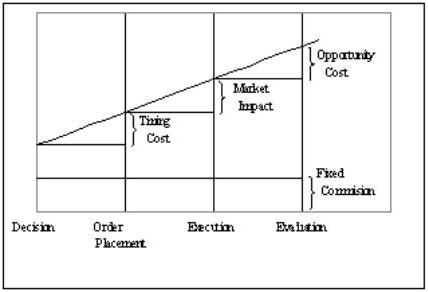
\includegraphics[width=10cm,height=6cm]{fg_i0n.png}
\end{center}
\caption[Decomposition of Implementation Shortfall Method]{{\bf Decomposition of Implementation Shortfall Method.}
\quad Trading costs are decomposed into four components, fixed commisions, timing cost, market impact, and opportunity cost.  ($x$-axis is time and $y$-axis is stock price.)}\label{fg_i0}
\end{figure}

In practice, there are several trading methods in which trading cost occurs in different fashions as shown in Table \ref{table_i1}.  We can also classify these trading methods into fixed-price trades and VWAP trades.  Fixed-price trades are regarded as trades in which execution price is determined explicitly at the trade execution.  Therefore, fixed-price trades include portfolio and block trades, market orders, and limit orders.  Since fixed-price trades tend to suffer larger market impact, execution of large trades should be divided into small orders.  However, fixed-price trades are frequently used by traders who can monitor and respond to the market quickly because traders can optimise fixed-price trades strategy explicitly.

Alternatively, VWAP trades are the second best approach because VWAP trades provide small trading costs and low price movement risks while not necessarily being optimal.  Although VWAP trades cannot be submitted and cancelled quickly because counterparts must agree with the terms and conditions of VWAP before the trades, VWAP trades are convenient methods for certain traders such as foreign investors and individual investors.  Therefore, there are mainly two approaches for saving trading costs: 
\begin{enumerate}
\item To balance the market impact and volatility risk by referring to a fixed price in portfolio or block trades.
\item To mitigate the impact of trades by referring to a volume weighted average price (VWAP henceforth) in VWAP trades.  
\end{enumerate}
These approaches are chosen according to trade size, traders' objectives, circumstances, and so forth.  For example, while Approach 1 has a direct effect on cost reduction, implementation has to be closely monitored during execution.  Therefore, foreign investors rather prefer Approach 2 in order to avoid market impact by completion of large orders under time difference .  Figure \ref{fg_i1} shows a sample flow chart for a choice of trading approaches and methods.

\begin{table}[htbp]
\begin{flushleft}
\begin{tabular}{|l||c|c|c|c|c|l} \hline
 & \multicolumn{4}{c|}{Cost} & & \quad \\ \cline{2-5}
 & Commission & Timing  & Market & Opportunity & Stability / & \quad \\
 & & cost & impact & cost & transparency & \\ \hline
 (Agency trade) & & & & & & \\
 Market order & medium & small & large & small & bad & \\
 Limit order & medium & small & small & large & good & \\
 VWAP trade & medium & medium & small--large & small & good--moderate & \\ \hline
 (Principal trade) & & & & & & \\
 Portfolio trade & large & large & N.A.\ & N.A.\ & moderate & \\
 Block trade & large & small & N.A.\ & N.A.\ & moderate & \\
 VWAP trade & medium & medium & small--large & N.A.\ & good--moderate & \\ \hline
\end{tabular}
\end{flushleft}

\begin{flushright}
\begin{tabular}{l|c|c|c||r|} \hline
 \quad & & & & \\
 & Handling / & Competitiveness & Others & \\
 & optimality & & & \\ \hline
 & & & & (Agency trade) \\
 & bad & bad & & Market order \\
 & good & bad & & Limit order \\
 & good & moderate & measure performance & VWAP order \\ \hline
 & & & & (Principal trade) \\
 & good & good & & Portfolio trade \\
 & good & good & & Block trade \\
 & moderate & good & & VWAP trade \\ \hline
\end{tabular}
\end{flushright}
\caption[Comparison of trading method]{{\bf Comparison of trading method.}
 \quad This table shows the advantages and disadvantages of the trading methods.
 Trading cost is decomposed according to the implementation shortfall method.
 Stability means that it is hard to affect the execution price by instantaneous supply and demand.
 Transparency means that execution price is hard to manipulate.
 Handling means that it is easy to add discretion.
 Optimality means that optimal execution can be expected.
 Competitiveness means that commission is competitive.}
\label{table_i1}
\end{table}

\begin{figure}[htbp]
\def\backsp{\hspace*{-1.5mm}}
\footnotesize{
%\[
\framebox[16.7cm][l]{
${\displaystyle
 \begin{array}{l}
 \quad \\
 \backsp\mbox{Trading Needs}
 \left\{
  \begin{array}{l}
   \backsp\mbox{Time difference}
   \left\{
    \begin{array}{l}
     \backsp\mbox{Large Trade}
     \left\{
      \begin{array}{ll}
       \backsp\mbox{Completion Required} & \rightarrow \mbox{\bf VWAP Trade} \\
       \backsp\mbox{Completion Not Required} & \rightarrow \mbox{\bf Limit Order}
      \end{array}
     \right.
     \\
     \\
     \backsp\mbox{Small Trade}
     \left\{
      \begin{array}{ll}
       \backsp\mbox{Completion Required} & \rightarrow \mbox{{\bf VWAP Trade} or {\bf Market Order}} \\
       \backsp\mbox{Completion Not Required} & \rightarrow \mbox{{\bf Limit Order} or {\bf Market Order}}
      \end{array}
     \right.
    \end{array}
   \right.
   \\
   \\
   \backsp\mbox{No Time difference}
   \left\{
    \begin{array}{l}
     \backsp\mbox{Confident in Execution}
     \left\{
      \begin{array}{ll}
      \multicolumn{2}{l}{
       \backsp\mbox{Large Trade}
       \left\{
        \begin{array}{ll}
         \backsp\mbox{Small Tracking Error} & \rightarrow \mbox{\bf Portfolio Trade} \\
         \backsp\mbox{Large Tracking Error} & \rightarrow \mbox{\bf Block Trade}
        \end{array}
       \right.}
       \\
       \backsp\mbox{Medium Trade} & \rightarrow \mbox{\bf VWAP Trade} \\
       \backsp\mbox{Small Trade} & \rightarrow \mbox{\bf Market Order}
      \end{array}
     \right.
     \\
     \\
     \backsp\mbox{Unconfident in Execution}
     \left\{
      \begin{array}{ll}
       \backsp\mbox{Large Trade} & \rightarrow \mbox{\bf Any Trade} \\
       \backsp\mbox{Small Trade} & \rightarrow \mbox{\bf Any Agency Trade}
      \end{array}
     \right.
    \end{array}
   \right.
  \end{array}
 \right.
 \\
 \quad \\
 \end{array}
}$
}
}
\caption[Flow chart for trading method selection]{{\bf Flow chart for trading method selection.}
 \quad This diagram shows a sample flow chart for a selection of the trading methods, based on comparison of the trading
 methods.}\label{fg_i1}
\end{figure}

This study proposes several optimal trade execution strategies based on the both approaches.  In Approach 1, we analyze a long-term execution scheduling problem and short-term order placement problem since it is difficult to analyze Approach 1 as a whole.  Also, in Approach 2, we analyze both static and dynamic optimization since static optimization works well for numerous small orders while dynamic optimization is more suitable for few large orders.  Therefore, the four cases below are analyzed in the subsequent chapters.

\bigskip

\noindent 1. Fixed-Price Trade
\begin{itemize}
\item Execution Schedule
\item Order Placement
\end{itemize}
\noindent 2. VWAP Trade
\begin{itemize}
\item Static Optimization
\item Dynamic Optimization
\end{itemize}

In practice, all securities trading are carried out through some type of trade execution, regardless of recognition.  At execution, one of the four approaches above is chosen according to the assets' characteristics and traders' objectives and circumstances.  In order to make an appropriate choice, traders have to deeply understand the nature of the alternatives.  

Although a few analyses have been made about the optimal trade execution based on findings of market microstructure, this study derives the optimal execution strategy in both fixed-price trades and VWAP trades, analyzes their characteristics, and provides guidance to the selection of these approaches.  Therefore, an extensive range of applications can be expected for any security trading activity.


\section{Fixed-Price Trade}\label{sec_i1}
\subsection{Execution Schedule}\label{sec_i11}
Konishi and Makimoto (2001) and Chapter \ref{chap_b} of this study, Optimal Slice of a Block Trade, analyze the static optimal execution schedule of fixed-price trades by variational methods.  Traders generally suffer large market impact in immediate execution while they avoid price movement risk.  Therefore, block trades are executed over a considerable duration to balancing market impact and price movement risk.  This study sets objective function as the sum of linear market impact and price movement risk multiplied by a conversion factor.  This value has two economic insights: total cost for traders where the conversion factor is the risk premium, the extent of risk averseness, and value at risk (VaR) for risk managers where the conversion factor is set according to the confidence interval.  This study then, derives analytically the minimal trading cost strategy of liquidation of a portfolio by variational methods.  VaR type risk measurement is widely used because the economic implication is intuitive and because risks of different assets are comparable.  However, since VaR cannot be additive in time, we employ static optimization but not dynamically optimizing.  

The optimal strategies derived by existing studies such as Almgren and Chriss (1999) have the unrealistic property that the time scale of optimal trading is independent of the initial portfolio size although intuition suggests that larger portfolios should trade more slowly and that total execution costs should grow superlinearly with portfolio size.  In contrast, our model has several advantages over existing studies.  First, we succeeded in making optimal execution duration an endogenous increasing function of whole trading size.  Second, the transaction cost of our strategy grows superlinearly with whole trading size, consistent with intuition.  Third, our results are immediately applicable to existing risk management frameworks and provides an explicit solution for minimum liquidity adjusted VaR (L-VaR).  Although this study uses an example of liquidation of a block of common stock, results can also be extended over wider problems on liquidation of any large block of assets.


\subsection{Order Placement}\label{sec_i12}
Chapter \ref{chap_l} of this study, Selection of Market and Limit Order, analyzes the dynamic optimal order placement strategy of fixed-price trades by dynamic programming.  Market and limit orders are frequently submitted and canceled and sometimes switched with each other as market price moves and probability of limit order execution changes.  However, since the execution price and volume of limit orders are non-linear, the economic effect and the optimal order placing strategy is not trivial, and few preceding studies can be found.  Therefore, this study analyses the optimal selection of market and limit orders in a series of single price batch auctions when the expectation of the limit order book is given.  

This study derives the analytical solution of a single limit order model for risk neutral traders by dynamic programming, and then extends the result for risk averse traders.  We find that the limit order size is independent of the whole trade size while the limit order price and the market order size are linear functions and that market orders replace limit orders as time passes.  Further, we calculate the economic value of monitoring the limit order book.


\section{VWAP Trade}\label{sec_i2}
\subsection{Static Optimization}\label{sec_i21}
Konishi (2002) and Chapter \ref{chap_s} of this study, Optimal Slice of a VWAP Trade, analyze the static optimal execution strategy of VWAP trades by an iteration of a single variable optimization.  VWAP trades are overtaking fixed-price trades in numerous trades including foreign investments because of low cost, high transparency, and capability of performance measurement.  Because VWAP trades are labor intensive, automatic execution of a static optimal strategy is often employed for trades with small risk.  

Although a few analyses have been made on the optimal execution of VWAP trades, this study derives analytically the static optimal execution strategy that minimizes the expected squared execution error when market price, price volatility, and market volume is stochastic.  This method is powerful because the optimal execution strategy is determined by an iteration of a single variable optimization, rather than by a multivariable optimization.  Analytical solutions are derived in some cases.  We show that optimal execution times tend to lag behind expected market trading volume distribution since price volatility has a positive correlation with market trading volume.  In a basket trade, execution error can be reduced by spreading out execution times according to the correlation of price movement.  We confirm our theoretical results with actual trading data and simulations.


\subsection{Dynamic Optimization}\label{sec_i22}
Chapter \ref{chap_d} of this study, Dynamic Optimal Slice of a VWAP Trade, further analyzes the dynamic optimal execution strategy of VWAP trades by dynamic programming.  It is feasible to reduce the execution error with a dynamic optimal strategy if a trader picks up a few stocks, monitors VWAP(of the market and the trader), and forecasts the future price movement and trading volume.  This study models the stochastic structure of market volume, and derives an approximation on optimal execution strategy with dynamic programming.  

This analysis confirms execution error reduction by actual trading data.  We find that even if market trading volume surges due to news, or other reasons, the trader should hold his execution rather than follow market execution.  If either buy or sell order is not allowed, execution becomes slower than in the case in which both are allowed.


\bigskip

\section{Closing Remarks}\label{sec_i3}
Although a few analyses have been made about the optimal trade execution based on findings of market microstructure, this study derives the optimal execution strategy in both fixed-price trades and VWAP trades, analyzes their characteristics, and provides guidance to the selection of these approaches.  Therefore, an extensive range of applications can be expected for any security trading activity.

This study is organized as follows.  First, Chapter \ref{chap_r} surveys relevant existing studies.  Chapter \ref{chap_b} to Chapter \ref{chap_d} analyze the optimal execution strategies of the four cases described above.  Finally, Chapter \ref{chap_c} concludes this study.

%%%%%%%%%%%%%%%%%%%
%Research Survey%%
%%%%%%%%%%%%%%%%%%%

\chapter{Research Survey}\label{chap_r}

\section{Introduction}\label{sec_r1}
Market microstructure is the study of the process and outcomes of exchanging assets among financial intermediations and institutions of exchange.  As is suggested by its name, the study of market microstructure has been developed along with the expansion of practical business needs under explicit trading rules and objectives.  Although the study of market microstructure spreads over various issues from macroscopic to microscopic as well as from theoretical to empirical, we would like to illustrates two large issues, market design in Section \ref{sec_r2} and optimal strategy in Section \ref{sec_r3}, which are most relevant to this study.

Looking at the history of investment business and research, we can see several stages.  First, the modern portfolio theory has been established in 1960's and developed in 1970's.  The greatest academic achievements include studies on the long-term equilibrium of financial markets, such as Portfolio Selection by Markoviz (1959), Capital Asset Pricing Model by Sharpe (1970), and Arbitrage Pricing Theory by Ross (1976).  These concepts provided great progress on the investment management, and as a consequence, portfolio investment was introduced and gradually took over investment on individual securities.  However, this is also the start of the long lasting argument on the gap between academic research and practical business partly because the practical market is sometimes far away from the equilibrium.

Since the deregulation of the Securities markets such as May Day in 1975 in the U.S.A. and Big Bang in 1986 in the U.K., trading activity has burgeoned.  This has led to a widening of the gap between the ideal equilibrium market and the practical market to the extent that it can no longer be considered negligible.  Consequently, the need for efficient market design was inevitable, and this gave birth to the study of market microstructure; an analysis of the dynamics of price formation.


%%%%%%%%%%%%%%%%%%%%%%%%
\section{Market Design}\label{sec_r2}
In this study area, empirical studies preceded theoretical studies in order to verify practitioners' feelings that the real market could not be explained by existing finance theories.  Then, theoretical studies of general equilibrium followed to provide descriptive explanations to these empirical findings.

Regardless of empirical and theoretical, the main parameters in market microstructure are price and quantity, just as the existing studies on price formation in micro economics.  Especially, market microstructure analyzes dynamical mechanisms, these parameters often appears as the change of price or volatility, and trading volume flow, which is henceforth referred as trading volume for simplicity.  

Due to the restriction of data and analytical tools, earlier studies observe these two parameters separately in the form of volatility and trading volume, which we call studies on market pattern and explain in Subsection \ref{subsec_r21}.  Later studies tied individual trades and price changes, and observe market impact, which are reflected in Subsection \ref{subsec_r22}.  Further, most of the existing studies are on quote driven markets because market data on order driven markets is too complex.  However, we pick up some among a few papers on order driven markets in Subsection \ref{subsec_r23} since the understanding of quote driven market is necessary for Chapter \ref{chap_l} of this study.


\subsection{Market Pattern}\label{subsec_r21}
%from(2.3.1)
It is known that some patterns exist in actual price and liquidity, which cannot be explained by existing finance theories.  For example, Jain and Joh (1988) analyze trading data of NYSE stocks from 1979 to 1983 and report the ``U-shaped effect" that trading volume is concentrated at the opening and closing of trading sessions, that trading volume on Monday is lower than on other days of the week while weekday pattern is smaller than intraday pattern, and that trading volume is closely related to price movement four hours before, which suggests effect of price movement lasts for a while.

Further, McInish and Wood (1992) analyze the intraday pattern of quote spread on the NYSE.  They find that quote spread tightens when trading is active.  Also, quote spread is larger for larger orders and smaller for more competitive markets to market makers.  While they also confirm the ``U-shaped effect" in the intraday pattern at NYSE, quote spread in a quote driven market such as NASDAQ and London Stock Exchange (LSE) remains large throughout the day, and tightens rapidly towards the closing.  Therefore, they conclude that difference in trading mechanism causes intraday pattern of quote spread.

Then, Chan et al. (1995) study quote spread of individual market makers and inside spread (difference between best quotes) for NASDAQ stocks.  They find that individual quote spread remains stable throughout the day and reveal that decline of inside spread at closing is due to heterogeneity of quote spread among market makers to unwind their positions.  Further, Barclay et al. (1999) find that after NASDAQ reform in which public traders became able to submit limit orders, NASDAQ shows the ``U-shaped effect" as NYSE.

Numerous studies have been done on the relationship between price volatility and market trading volume since Clark's (1973) seminal paper, including Epps and Epps (1976), Tauchen and Pitts (1983).  Karpoff (1987) summarizes these results, and Andersen (1996) proposes a modified model.  These studies, in general, support the existence of a positive correlation between price volatility and market trading volume and the autocorrelation of themselves because surprising news boosts both price volatility and market trading volume.  

Regarding Japanese markets, Kawahara and Murase (1993) analyze intraday data of TSE stocks in 1993.  They attribute factors of price movement within a day into quote spread, execution period, and trading volume.  

On the theory side,
%from(2.4-2.4.1)
 trade models are devised in order to provide customary market designs and patterns with theoretical grounds.  Market participants in the real world do not always have all the public information and behave rationally, but act with different information, objectives, and circumstances.  Therefore, real markets are too complex to analyze.  As a result, existing trade models employ significantly simplified assumptions on the roles and objectives of market participants, and try to obtain qualitative implications.  

%\subsection{Strategic Trader Model}
One of the pioneering works is done by Kyle (1985), who assumed that traders submit market orders, and then market makers settle the surplus of traders' orders and determine the price.  According to this model, the excess demand of the informed trader is larger when volatility of settlement price is lower and when uncertainty of noise trader is higher.  Also, quote spread is smaller when the volatility of settlement price is lower and when uncertainty of the noise trader is higher.  Further, this study specifies the abstract idea of market liquidity as 1) existence of quote, 2) small quote spread, 3) capability of successive trades, and 4) capability of instantaneous execution of large trade.  Liquid market thus represents an efficient market in the sense that orders of any size are tradable instantaneously around market prices.

Admati and Pfeiderer (1988) analyze a multiple period model in order to explain the ``U-shaped effect."  They show that orders by uninformed traders tend to cluster in the period with more informed traders such as opening and closing, and price volatility also increases.  

Subrahmanyam (1991) assumes riskaverse informed traders and finds that informed traders reduce orders to avoid risks from noise traders, and therefore, price does not reflect information effectively.

%%%%%%%%%%%%%%%%%
\subsection{Market Impact}\label{subsec_r22}
%from(2.3.2)
Market impact measures the extent to which short-term liquidity makes execution prices diverge from long-term fundamental prices. Holthausen et al. (1987) analyse block trades, and find that prices move in the opposite direction after block trades.  They conclude that block orders not only introduce new information to adjust price levels but also bring temporary price turbulence due to low liquidity and speculations.  As a result, they distinguish temporary impact and permanent impact.  

Also, Hausman et al. (1992) focuses on discreteness of execution price and estimate market impact precisely with an ordered probit model.  Further, BARRA (1997) develops a practical market impact model whose impact is an increasing function of trade size and the marginal increase is a decreasing function.  BARRA's model attributes market impact to individual factors (price elasticity of quote, volatility, number of ticks, and trading size) and market factors.

Since analysis on market impact was born in the United States, where quote driven markets are prevailing, there are few studies on order driven markets.  It is difficult to identify block orders from trading data in an order driven market since trading data is merely a sequence of times, prices and volumes of ticks which are split into single limit orders on the limit order book. In addition trading data does not show lumps or the direction of orders.

Uno and Yamada (1993) analyze intraday data of TSE stocks.  They regard down-ticks as sell orders and up-ticks as buy orders and aggregate net buy orders into five-minute intervals.  They explained market impact is determined by long-term characteristics of the asset such as average trading volume and volatility and short-term characteristics of trading such as tick trend, trading volume, and the depth of the limit order book.

\subsection{Limit Order}\label{subsec_r23}
Most of the existing studies are on quote driven markets because market data in order driven markets is too complex.  However, we pick up some among few papers on order driven markets in this subsection since the understanding of quote driven market is necessary for Chapter \ref{chap_l} of this study.

%from(4.1)
Market and limit orders are two essential instruments of order placement.  Progress in information technology has improved order processing capability and made order placement strategy a critical issue in investment.  For example, order driven markets such as the Tokyo Stock Exchange (TSE) have excluded floor traders and adopted automatic matching systems, which makes order processing faster and less error prone.  Also, several markets such as New York Stock Exchange (NYSE) and National Association of Securities Dealers Automated Quotation System (NASDAQ) started allowing limit orders, to broadening traders' order placement options.  Further, emergence of alternative trading systems such as crossing networks and electronic communication networks have enabled traders to tactically submit and cancel orders across markets.  In practice, traders recognize the advantage of limit orders: cost efficiency, and disadvantages: uncertain execution and free option, and choose either market or limit order or sometimes both as it fits their objectives and circumstances.  

Several empirical studies confirm traders' behavior in the real market.  For example, 
%from(2.3.3)
Biais et al. (1995) analyze trading data of Paris Stock Exchange, an order driven market, and find that traders are affected by limit order books and trades just before the order submission.  Especially, more market orders are submitted when the bid-ask spread is small, and more limit orders are submitted inside the bid-ask spread when the bid-ask spread is large, which suggests that traders sufficiently consider the execution probability of limit orders.

Harris and Hasbrouck (1996) analyze data of NYSE and calculate that execution probability of limit orders within the bid-ask spread is 60\%.  They show that trading cost of limit orders is lower than other strategies when bid-ask spread is wide, which is consistent with the result of Biais et al. (1995).

Regarding the Japanese market, Kawahara (1994) analyzes TSE stock data in 1994 and finds that the trading cost of limit orders outside the best bid and ask prices is 0.15\% lower than that of market orders.  Also, that the trading cost is larger for sell orders, large orders, and limit orders with shorter exposure to the market.

In contrast, theoretical studies are limited for the selection of market and limit orders.  For example, although Bertisimas and Lo (1998) and Chapter \ref{chap_b} of this study derive the optimal order slicing strategy in a large portfolio liquidation, only market orders but no limit orders are allowed in their models.  Also, Parlour (1999) analyses how market conditions affect the selection of market and limit orders when a trader places just one unit of order.  This analysis shows the interaction between trader's order placing strategy and market conditions, but fails to study how traders split orders for large trades.  Further, Chakravarty and Holden (1995) provide a theoretical model which explains how traders select market and limit orders in a quote driven market.  However, existence of a market maker is crucial in their model, and the results are not directly applicable to an order driven market.  Accordingly, Chapter \ref{chap_l} of this study analyzes the optimal selection of market and limit orders, sizes, prices, and times in a series of single price batch auctions.  

\subsection{Closing Remarks}\label{subsec_r24}
%from(2.3.4)
Empirical studies successfully reveal practical market anomalies.  Especially, it is shown that market and limit orders should be chosen depending on market circumstances and traders' objectives although these orders should be indifferent theoretically in an efficient market.  However, analysis on order driven markets has just been started, and numerous issues are left for further analysis since the trading data is complex and disclosure has not been sufficient and also since most exchanges in the United States where research on market microstructure was born are quote driven market.

%from(2.4.4)
On the theory side, trade models successfully reveal the roles of market participants and show the conditions in which market stability is retained.  However, the models are significantly simplified in order to avoid complexity, and therefore, reflection of the practical market is left for succeeding researches of the optimal strategy, which are explained in Section \ref{sec_r3}.

%%%%%%%%%%%%%%%%%%%
\section{Optimal Strategy}\label{sec_r3}
In the 1990's, world equity market parcipitants prosperedwhile market prices trended higher.  These conditions favoured the birth of numerous hedge funds.  Investment business has become more competitive, and trade execution has attracted more attention.  With the deep understanding of market mechanisms brought by previous studies on market designs, the study of market microstructure has been revealed to be another large issue of the optimal strategy.
Whereas theoretical models in market design tend to use qualitative analysis and general equilibrium, theories in optimal strategy lend themselves more towards quantitative analysis and the partial equilibrium approach.

The first major task is the conceptual definition of trading cost by
Perold (1988), which is explained in Subsection \ref{subsec_r31}.  With this trading cost in mind, earlier theoretical studies try to determine the optimal portfolio with specific forecast, which is explained in Subsection \ref{subsec_r32}.  After trade execution is recognized as an independent function, we saw several studies on the optimal execution as explained in Subsection \ref{subsec_r33}.

\subsection{Trading Cost}\label{subsec_r31}
%from(1)
According to the ``implementation shortfall method" by Perold (1988), the standard framework of market microstructure analysis, trading costs are defined as difference between the market price at the time of decision-making and evaluating price. The evaluating price consists of the executed price of the filled order and the evaluating price of the unfilled order.  Further, trading costs are decomposed into four components, fixed commisions, timing cost, market impact, and opportunity cost as we see in Figure \ref{fg_i0}.  Among them, timing cost is the difference between market price at the time of decision-making and time of order placement. Market impact is the difference between market price at the time of order placement and the executed price, which is caused by the relationship between trading volume and price change. Lastly opportunity cost is the difference between the executed price and the evaluating price of unfilled order.  Strictly speaking, the nature of timing cost and opportunity cost is the price movement risk but is not necessarily a loss.  However, the price movement risk is often recognized as cost after being mulitiplied with a conversion factor, a risk premium, because most traders are risk averse.  Trade execution strategy can control market impact and price movement risk.

\subsection{Optimal Portfolio Selection}\label{subsec_r32}
%from(2.5.1)
Konno and Wijayanayake (1998) develop a mean absolute difference model in order to build optimal rebalance portfolio under a non-linear trading cost function.  They take into account trading costs for rebalance (difference between existing and optimized portfolio) in addition to expected return and risk as usual. Generally, average trading cost is large for small orders, and decreases as trade size increases.  However, over large trades tighten order supplies and increase trading cost again.  As a result, average trading cost is a ``reverse S-shaped" function of trade size.

In order to solve this complicated optimization numerically, this study measures price movement risk in absolute difference and approximates trading cost as a piecewise linear function, which simplifies the problem into piecewise linear programming.

\subsection{Optimal Execution}\label{subsec_r33}
%from(3.1)
In various aspects of financial decision-making from risk management to trading, it is commonly assumed that any trade can be executed around a prevailing price within a short period of time.  However in practice, we sometimes face situations in which market cannot fully absorb all the trading needs of a large portfolio.  In such cases, asset liquidity risk, defined as the potential deviation between market price and executed price, becomes significant.  Liquidity risk has attracted much attention since the LTCM 1998 disaster, as described in Jorion (2000).  Conventional VaR measures should be extended to account for liquidity risk as well as optimal trading strategies.  This leads to the concept of L-VaR, a liquidity-adjusted risk measure. 

Since asset liquidity risk is a highly complicated problem, there used to be a large gap between practice and theory.  On the practice side, it is known that in liquidation of a block trade portfolio, traders generally divide the whole trade into small orders in order to reduce the cost.  In doing so, it is common to take a longer time for larger trades.  Also, BARRA (1997)'s analysis on quote driven market and Mannen and Uno (2000)'s analysis on order driven market show that the quoted premium of a block trade in the real market is an increasing function of whole trading size, and that the marginal increment is a decreasing function (i.e., the first derivative is positive and the second derivative is negative).  

On the theory side, Collins and Fabozzi (1991) proposed a conceptual framework, which decomposes trading cost into execution cost and opportunity cost.  According to their research, quick execution suffers huge execution cost, while slow execution creates large opportunity cost from price movement risk.  Therefore a trader chooses the best strategy that balances these two factors in determining execution schedule.

Subsequent studies investigated more detailed theory.  Bertsimas and Lo (1998) derived the optimal execution strategy of a large block of common stock over a fixed time horizon by dynamic programming.  However, they analyzed only risk neutral traders because of computational complexity of dynamic programming.  So, they just minimized the expectation value of execution cost, but did not consider price movement risk, and therefore, no reasonable guidance on the duration of execution was provided.  On the other hand, Grinold and Kahn (1999) and Almgren and Chriss (1999) took the sum of execution cost and opportunity cost of the whole trade, as the objective function to minimize, and derived a static optimal execution strategy.  Although they studied risk averse traders, optimal execution duration and average cost are still independent of whole trading size, which contradicts the result of BARRA (1997) and Mannen and Uno (2000).  Further, Grinold and Kahn (1999) contradicts their own statement that risk increases as square root of time, since their risk measured in variance, in fact, increases linearly.  This is crucial because the time dependency of cost and risk determines the optimal execution strategy.

To the contrary, in order to bridge the gap between theory and practice, this chapter modifies objective function in a practical manner, which reflects the reality of the order driven market, and obtains a reasonable relationship between transaction cost and whole trading size.  Specifically, we extend the results on optimal execution strategy derived by Grinold and Kahn (1999) and Almgren and Chriss (1999).  As mentioned above, the explicit solutions obtained in the earlier work have the unrealistic properties in that the time scale of optimal execution strategy is independent of whole trading size, and the total cost of trading is linear in whole trading size. 

There are two possible ways to capture these effects in a quantitative model. One way is to modify the cost functions to be nonlinear.  Another way is to change the weighting of cost uncertainty from a mean-variance model based on a smooth utility function, to a penalty based on standard deviation, which is more in the spirit of VaR models.  This approach was briefly discussed in Almgren and Chriss (1999) where it was observed that solutions could be obtained graphically on the efficient frontier, but explicit solutions were not obtained due to the nonlinearity of the problem, nor were the properties of these solutions explored.

For the standard deviation model, our study in Chapter \ref{chap_b} derives explicit solutions of optimal execution strategy under asset liquidity risk.  It extends the work of Almgren and Chriss (1999), who derive a measure of L-VaR.  We obtain explicit solutions both for the single-asset case and for a multi-asset portfolio model in the form of pure exponentials.  The explicit form obtained for the coefficients shows that the characteristic time increases as whole trading size to the two-thirds power, and total cost increases as whole trading size to the four-thirds power, both consistent with intuition.

%from(6.1)
Optimal execution is very important in both fixed-price and VWAP trades.  It is true that VWAP has become an industry standard, and that numerous studies have been done on market pattern as we have seen in Subsection \ref{subsec_r21}, and that several studies have been made on optimal strategies for general trade execution.  However, little academic work can be found on the optimal execution of VWAP trades.  Therefore, Chapter \ref{chap_s} and \ref{chap_d} analyze the static and dynamic optimal execution of VWAP trades, respectively.

\subsection{Closing Remarks}\label{subsec_r34}
%from(2.5.3)
Previous studies successfully balance market friction and traders' objectives, which is not addressed by existing finance theory.  However, for analytical feasibility, most studies are too simplified and sometimes inconsistent with market practice.  Further, there are several trading methods in practice.  Policies which suggests how to select appropriate trading method according to asset characteristics and traders' objectives and circumstances are left for further analysis.
%from(1.3)
In practice, all the security trading is carried out through some trade execution, regardless of recognition.  At execution, one of the four approaches above is chosen according to assets' characteristics and traders' objectives and circumstances.  In order to make an appropriate choice, traders have to deeply understand the nature of the alternatives.  

Although few analyses have been made about the optimal trade execution based on findings of market microstructure, this study derives the optimal execution strategy in each approach, analyzes its characteristics, and provides the guidance to the selection of these approaches.  Therefore, an extensive range of application can be expected for any security trading.

% 02/01 moved Lemma 3.3.2 to Section 3.7
% 02/01 changed according to ref No.2
% 02/05 changed from .emf to n.png
% 02/06 changed according to ref No.2 (by Makimoto)

%%%%%%%%%%%%%%%
%   Block    %%
%%%%%%%%%%%%%%%
\chapter{Optimal Slice of a Block Trade}\label{chap_b}

%%%%% local definition
\def\keymtx{\A^{-1}\S}

%%%%%%%%%%%%%%%%%%%%%%
%\newpage

%\vspace*{0.5cm}

%\begin{center}
%{\large {\bf Optimal Slice of a Block Trade}}
%\end{center}

%\vspace*{0.5cm}

\begin{quote}
{\bf Abstract} \quad In liquidation of a block trade, it is common to divide execution in order to minimize total transaction cost, balancing market impact costs and volatility effects.  This chapter formulates the execution scheduling as a static optimization problem assuming linear market impact and derives explicit solutions. We show that optimal execution duration and average cost are increasing functions of the initial portfolio size, which is consistent with trading practice and empirical studies.  Our model provides explicit solutions for minimum liquidity adjusted value at risk (L-VaR), which is particularly useful for risk management.

\vspace*{0.5cm}

\end{quote}

%%%%%%%%%%%%%%%%%
\section{Introduction}\label{sec_b1}

In various aspects of financial decision-making from risk management to trading, it is commonly assumed that any trade can be executed around a prevailing price within a short period of time.  However in practice, we sometimes face situations in which market cannot fully absorb all the trading needs of a large portfolio.  In such cases, asset liquidity risk, defined as the potential deviation between market price and executed price, becomes significant.  Liquidity risk has attracted much attention since the LTCM 1998 disaster, as described in Jorion (2000).  Conventional VaR measures should be extended to account for liquidity risk as well as optimal trading strategies.  This leads to the concept of L-VaR, a liquidity-adjusted risk measure. 

This chapter derives explicit solutions of optimal execution strategy under asset liquidity risk.  It extends the work of Almgren and Chriss (1999), who derive a measure of L-VaR.  Almgren and Chriss obtain optimal execution strategies by considering the trade-off between immediate liquidation, which entails no price risk but has high market impact, and slow liquidation, which minimizes market impact but exposes the portfolio to price risk.  Their approach, however, has the unrealistic property that the time scale of optimal trading is independent of the initial portfolio size.  Intuition suggests that larger portfolios should trade more slowly and that total execution costs should grow superlinearly with portfolio size.

In contrast, our model has several advantages.  First, we succeeded in making optimal execution duration an endogenous increasing function of whole trading size.  Second, our transaction cost grows superlinearly with whole trading size, consistent with intuition.  Third, our results are immediately applicable to existing risk management framework and provides explicit solution for minimum L-VaR.  Also, although this chapter uses an example of liquidation of a block of common stock, results can be extended over wider problems on liquidation of any large block of assets.

Since asset liquidity risk is a highly complicated problem, there used to be a large gap between practice and theory.  On the practice side, it is known that in liquidation of a block trade portfolio, traders generally divide the whole trade into small orders in order to reduce his cost.  In doing so, it is common to take a longer time for larger trades.  Also, BARRA (1997)'s analysis on quote driven market and Mannen and Uno (2000)'s analysis on order driven market show that the quoted premium of a block trade in the real market is an increasing function of whole trading size, and the marginal increment is a decreasing function (i.e., the first derivative is positive and the second derivative is negative).  

On the theory side,  Collins and Fabozzi (1991) proposed a conceptual framework, which decomposes trading cost into execution cost and opportunity cost.  According to their research, quick execution suffers huge execution cost, while slow execution creates large opportunity cost from price movement risk.  Therefore a trader chooses the best strategy that balances these two factors in determining execution schedule.

Subsequent studies investigated more detailed theory.  Bertsimas and Lo (1998) derived the optimal execution strategy of a large block of common stock over a fixed time horizon by dynamic programming.  However, they analyzed only risk neutral traders because of computational complexity of dynamic programming.  So, they just minimized the expectation value of execution cost, but did not consider price movement risk, and therefore, no reasonable guidance on the duration of execution was provided.  On the other hand, Grinold and Kahn (1999) and Almgren and Chriss (1999) took the sum of execution cost and opportunity cost of the whole trade, as the objective function to minimize, and derived a static optimal execution strategy.  Although they studied risk averse traders, optimal execution duration and average cost are still independent of whole trading size, which contradicts the result of BARRA (1997) and Mannen and Uno (2000).  Further, Grinold and Kahn (1999) contradicts their own statement that risk increases as square root of time, since their risk measured in variance, in fact, increases linearly.  This is crucial because the time dependency of cost and risk determines the optimal execution strategy.

 To the contrary, in order to bridge the gap between theory and practice, this chapter modifies objective function in a practical manner, which reflects the reality of the order driven market, and obtains a reasonable relationship between transaction cost and whole trading size.  Specifically, we extend the results on optimal execution strategy derived by Grinold and Kahn (1999) and Almgren and Chriss (1999).  As mentioned above, the explicit solutions obtained in the earlier work have the unrealistic properties that the time scale of optimal execution strategy is independent of whole trading size, and the total cost of trading is linear in whole trading size. 

There are two possible ways to capture these effects in a quantitative model. One way is to modify the cost functions to be nonlinear.  Another way is to change the weighting of cost uncertainty from a mean-variance model based on a smooth utility function, to a penalty based on standard deviation, which is more in the spirit of VaR models.  This approach was briefly discussed in Almgren and Chriss (1999) where it was observed that solutions could be obtained graphically on the efficient frontier, but explicit solutions were not obtained due to the nonlinearity of the problem, nor were the properties of these solutions explored.

For the standard deviation model, we obtain explicit solutions both for the single-asset case and for a multi-asset portfolio model in the form of pure exponentials.  The explicit form obtained for the coefficients shows that the characteristic time increases as whole trading size to the two-thirds power, and total cost increases as whole trading size to the four-thirds power, both consistent with intuition.

The biggest problem with this VaR-type weighting of risk is that the solutions  do not satisfy the ``principle of optimality": solutions computed statically at the start of trading are no longer optimal if reevaluated in the course of execution. Although formally this makes the solutions invalid, and calls for the use of a dynamic programming method, these solutions are useful in practice because of the following advantages:
\begin{itemize}
 \item Statically optimized execution can be used as a benchmark, i.e., actual trading strategy
might be changed as new information arrives and the performance of a strategy change can be
evaluated by comparing the cost to that of static optimal execution strategy.
 \item Statically optimized execution is sometimes a reasonable choice in program trading, i.e., it is
technically difficult to record all the history of price and profit and change the strategy
dynamically especially in a portfolio trade.  Therefore, static optimal execution strategy is a good
alternative in practical trading.
\end{itemize}

This chapter is organized as follows.  In the next section, we formulate the cost minimization problem.  Section \ref{sec_b3} is devoted to derive the optimal execution strategy for general case.  The case when we have limit to the volume executable instantaneously is studied in Section \ref{sec_b4}.  Section \ref{sec_b5} discusses the principle of optimality.  Finally in Section \ref{sec_b6}, we conclude the analysis.

%%%%%%%%%%%%%%%%%%%%%%%%
\section{Formulation of Optimization}\label{sec_b2}

 Let $(\Omega, \calF, Q)$ be a probability space with a filtration $\{ \calF_t \}$ which satisfies usual conditions.  Suppose we would like to liquidate a portfolio of $N$ assets and whole trading size of asset $i$ is $V_i\ (i=1,\cdots,N)$.  Let $P_i(t)\ (i=1,\cdots,N)$ denote $\{ \calF_t \}$-adapted stock's fair value process.  Similar to the standard option pricing theory, the stock price process is assumed to follow standard Brownian motion with volatility $\sigma_i$ and correlation $\rho_{ij}$.  Drift term is considered to be zero because the time frame is short.
 So, the stock's fair value processes are represented as
\begin{eqnarray*}
  & & dP_i(t) = \sigma_i dB_i(t), \quad i=1,\cdots,N, \\
  & & dB_i(t) dB_j(t) = \rho_{ij} dt, \quad i,j=1,\cdots,N.
\end{eqnarray*}
 Let $v_i(t)\ (i=1,\cdots,N)$ denote the selling volume of asset $i$ at time $t$.
 Because of the order quantity constraints,
\begin{equation}\label{eq_b1}
  \int_0^\infty v_i(t) dt = V_i, \qquad i=1,\cdots,N.
\end{equation}

 In the rest of the chapter, we consider total transaction cost as the sum of execution cost and opportunity cost, and study the static minimization of transaction cost under this framework.  More precisely, we look for $v_i(t)$ which minimizes transaction cost among all trading strategy that is pre-determined at $t=0$.

 Regarding execution cost, the main factor that can be controlled by order slicing is market impact, the difference between observed price at the market and the stock's fair value.  Holthausen et al.~(1987) and Uno and Yamada (1993) say that market price tends to overshoot with a block trade, and therefore, market impact should be divided into temporary and permanent components.  Further, several features are known regarding the market impact in an order driven market, such as the Japanese market.  First, according to Copeland and Galai (1983), a limit order can be considered as a free option contract, and so, only a part of demand and supply are placed as limit orders at one time.  Therefore, a trader has to wait until orders on the opposite side appear.  Actually, Biais et al.~(1995) observed that there are few limit orders at prices far from the market price.  Second, while a quote driven market allows a trader to negotiate prices with a market maker according to trading volume, an order driven market does not have a function to negotiate price and trading volume, which forces traders to repeat small execution.  Also, if anonymity is guaranteed in an order driven market, repeating execution is thought to leak less information than a bulk execution.  

In summary, the advantages of order slicing are 1) avoiding temporary
market impact, 2) waiting for all the potential orders to appear, and 3)
concealing one's trade.  Therefore, this chapter separates market impact
into temporary and permanent component, sets a limit to the volume
executable instantaneously, and assumes each component to be a linear
function of trading volume within moderate volume and time.  Choice
between market order and limit order is certainly another important
factor in optimal execution.  However, this chapter regards it as a
tactical decision after the order slice is fixed, and excludes it from
the scope of the research since it is common to place orders only around
a prevailing price as mentioned above.  Specifically, we introduce
coefficients below.

\vspace{3mm}

\begin{tabular}{l}
 $a_i>0\ (i=1,\cdots,N)$ : temporary impact coefficient of asset $i$, \\ [3mm]
 $b_i>0\ (i=1,\cdots,N)$ : permanent impact coefficient of asset $i$.
\end{tabular}

\vspace{3mm}

\noindent Since temporary impact depends only on the momentary trade and permanent impact depends on the accumulated volume traded up to that moment, total market impact at time $t$ can be represented as
\[
  \sum_{i=1}^N v_i(t) \left\{ a_i v_i(t) + b_i \int_0^t v_i(s) ds \right\}.
\]
 Therefore, market impact over the execution period becomes
\begin{eqnarray}
  \mbox{(market impact)}
  & = & \int_0^\infty \sum_{i=1}^N v_i(t) \left\{ a_i v_i(t) + b_i \int_0^t v_i(s) ds \right\} dt \nonumber \\
  & = & \int_0^\infty \v(t)^\top \A \v(t) dt +\frac{1}{2} \V^\top \B \V \label{eq_b16}
\end{eqnarray}
where $\v(t)=(v_1(t),\cdots,v_N(t))^\top$, $\V=(V_1,\cdots,V_N)^\top$,
$\A = \mbox{Diag}(a_1,\cdots,a_N)$, $\B= \mbox{Diag}(b_1,\cdots,b_N)$.
 Here, $\mbox{Diag}(z_1,\cdots,z_N)$ denotes an $N \times N$ diagonal matrix whose diagonal element is
$z_i\ (i=1,\cdots,N)$ and $\top$ denotes transpose.

 Meanwhile, regarding opportunity cost, price movement risk is often measured by a multiple of standard deviation as VaR, which has the same dimension as the price itself.  This risk measurement has the following advantages:
\begin{itemize}
 \item A trader can evaluate the appropriateness of the trade by estimating risk as VaR, i.e., he compares the maximum loss of the block trade and his risk tolerance, and judges before the trade whether he can assume the risk.
 \item A trader can evaluate the profitability of the trade, i.e., if a trader requires a profit greater than Sharp ratio (return over standard deviation) $\lambda$, the premium $p$ should be
\[
  p > \mbox{(market impact)} + \lambda \mbox{(opportunity cost)}
\]
since
\[
  \frac{p - \mbox{(market impact)}}{\mbox{(opportunity cost)}} > \lambda.
\]
\end{itemize}

Specifically, we define opportunity cost as standard deviation of fair sales value.  Total fair value of the whole execution is
\begin{eqnarray*}
  \sum_{i=1}^N \int_0^\infty v_i(t) P_i(t) dt
     & = & \sum_{i=1}^N \int_0^\infty v_i(t) \left\{ P_i(0) + \int_0^t dP_i(s) \right\} dt \\
     & = & \sum_{i=1}^N \left\{ V_iP_i(0) + \int_0^\infty x_i(t) dP_i(t) \right\} \\
     & = & \sum_{i=1}^N \left\{ V_iP_i(0) + \sigma_i \int_0^\infty x_i(t) dB_i(t) \right\}
\end{eqnarray*}
where $x_i(t)=\int_t^\infty v_i(s) ds$.
 So, standard deviation is given by
\begin{eqnarray}
  \sqrt{\ex{\left( \sum_{i=1}^N \sigma_i \int_0^\infty x_i(t) dB_i(t) \right)^2}}
   & = & \sqrt{ \int_0^\infty \sum_{i,j=1}^N \sigma_i \sigma_j \rho_{ij} x_i(t) x_j(t) dt } \nonumber \\
   & = & \sqrt{ \int_0^\infty \x(t)^\top \S \x(t) dt } \label{eq_b17}
\end{eqnarray}
where $\S = ( \sigma_i \sigma_j \rho_{ij}; i,j=1,\cdots,N)$ is a variance-covariance matrix of price processes and $\x(t)=(x_1(t),\cdots,x_N(t))^\top$.
 Therefore, opportunity cost can be defined as $\lambda \sqrt{ \int_0^\infty \x(t)^\top \S \x(t) dt }$ where $\lambda$ is the risk premium.

 Total transaction cost ($TC$) of a trader is the sum of execution cost and opportunity cost, and from (\ref{eq_b16}) and (\ref{eq_b17}),
\[
  TC = \int_0^\infty \x'(t)^\top \A \x'(t) dt +\frac{1}{2} \V^\top \B \V
            + \lambda \sqrt{ \int_0^\infty \x(t)^\top \S \x(t) dt }
\]
which can be divided into fixed cost ($FC$) and variable cost ($VC$),
\begin{eqnarray*}
  FC & = & \frac{1}{2} \V^\top \B \V, \\
  VC(\x) & = & \int_0^\infty \x'(t)^\top \A \x'(t) dt 
        + \lambda \sqrt{ \int_0^\infty \x(t)^\top \S \x(t) dt }.
\end{eqnarray*}
 Here, $\x=(\x(t), 0\leq t<\infty)$ and $\x'(t)=-\v(t)$ denotes
element-wise derivative.  In what follows, we assume $\x=(\x(t), 0\leq
t<\infty) \in \calC_\infty^2$ meaning that each component of
$\x(t)=(x_1(t),\cdots,x_N(t))^\top$ has continuous second derivative
$x_i''(t)$ and vanishes at infinity, i.e., $\lim_{t\rightarrow\infty}
x_i(t)=0$ and hence $\lim_{t\rightarrow\infty} x_i'(t)=0$.
 Therefore, regarding $VC(\x)$ as a functional of $\x$, our problem can be formulated as follows:
\[
  \mbox{(P)} \ \ \left|
  \begin{array}{ll}
    \mbox{minimize} & \quad VC(\x) \\ [2mm]
    \mbox{s.t.} & \quad \x =(\x(t), 0\leq t<\infty) \in \calC_\infty^2, \quad \x(0)=\V.
  \end{array}
  \right.
\]
 This definition is more practical than that of Almgren and Chriss (1999) in that the opportunity cost is measured by estimating standard deviation similar to VaR.  As we will see later, dimension of the market impact becomes larger than that of opportunity cost because of this definition, and the execution schedule becomes a function of whole trading size.

%%%%%%%%%%%%%%%%%%%
\section{Derivation of the Optimal Execution Strategy}\label{sec_b3}
 In order to derive the optimal slicing, we first prepare some preliminary results.  First, choose arbitrary strategy $\x = (\x(t), 0\leq t<\infty) \in \calC_\infty^2$ and let $\y=(\y(t), 0\leq t<\infty) \in \calC_{0,\infty}^2$ be any perturbation of $\x$ where $\y=(\y(t), 0\leq t<\infty) \in \calC_{0,\infty}^2$ means that each element $y_i(t)$ of $\y(t)=(y_1(t),\cdots,y_N(t))^\top$ has continuous second derivative and vanishes at $t=0$ and infinity, i.e., $y_i(0) = \lim_{t\rightarrow\infty} y_i(t) = 0$.  Then, a direct calculation shows
\begin{eqnarray*}
  \dif{}{\epsilon} VC(\x + \epsilon \y)
   & = & 2C + 2D\epsilon + \frac{\lambda (F + G \epsilon)}{\sqrt{E + F \epsilon +
         G \epsilon^2}}, \label{eq_b14} \\
  \ddif{}{\epsilon} VC(\x + \epsilon \y)
   & = & 2D + \frac{\lambda (EG-F^2)}{(E+F \epsilon + G \epsilon^2)^{3/2}} \label{eq_b15}
\end{eqnarray*}
where
\begin{eqnarray*}
  & & C = \int_0^\infty \x'(t)^\top \A \y'(t) dt, \qquad D = \int_0^\infty \y'(t)^\top \A \y'(t) dt, \\
  & & E = \int_0^\infty \x(t)^\top \S \x(t) dt, \qquad F = \int_0^\infty \x(t)^\top \S \y(t) dt, \qquad
  G = \int_0^\infty \y(t)^\top \S \y(t) dt.
\end{eqnarray*}
\begin{lemma}\label{lem_b2}
 \quad The equality
\begin{equation}\label{eq_b2}
  \left. \dif{}{\epsilon} VC(\x+\epsilon \y) \right|_{\epsilon=0} = 0
\end{equation}
holds for any $\y \in \calC_{0,\infty}^2$ if and only if $\x$ satisfies
\begin{equation}\label{eq_b3}
  \x''(t) = \frac{\lambda}{2\sqrt{E}} \keymtx \x(t), \qquad \forall t \in (0, \infty).
\end{equation}
\end{lemma}
\begin{proof} Since $\lim_{t\rightarrow\infty} \x'(t)=\0$ and $\y(0)=\0$,
\[
  C = \left[ \x'(t)\A\y(t) \right]_{t=0}^\infty - \int_0^\infty \x''^\top(t) \A \y(t) dt
    = - \int_0^\infty \x''^\top(t) \A \y(t) dt.
\]
 Then, we get
\[
  \left. \dif{}{\epsilon} VC(\x+\epsilon \y) \right|_{\epsilon=0} 
  = 2C + \frac{\lambda F}{\sqrt{E}}
  = 2 \int_0^\infty \left\{ -\x(t)''^\top \A + \frac{\lambda}{2\sqrt{E}}\x(t)^\top \S \right\} \y(t) dt.
\]
 Therefore, (\ref{eq_b2}) holds for arbitrary $\y \in \calC_{0,\infty}^2$ if and only if (\ref{eq_b3}) holds
since $\A$ is non-singular and both $\A$ and $\S$ are symmetry.
\end{proof}

\noindent The next lemma is concerned with the second order condition.
\begin{lemma}\label{lem_b3}
 \quad For any $\y \in \calC_{0,\infty}^2$,
\[ %begin{equation}\label{eq_b4}
  \ddif{}{\epsilon} VC(\x+\epsilon \y) \geq 0, \qquad \forall \epsilon \in (-\infty,\infty).
\] %\end{equation}
\end{lemma}

\begin{proof}
  See Section \ref{sec_bappendix}.
\end{proof}


 From Lemmas \ref{lem_b2} and \ref{lem_b3}, and the optimality criterion of the variational method, the optimization problem is reduced to finding $\x$ that satisfies (\ref{eq_b3}) and the boundary condition.  When there is only single asset, this problem is relatively easy.  Indeed, standard theory of differential equations shows that
\begin{equation}\label{eq_b21}
  x(t) = V e^{-\alpha t}, \qquad t \geq 0
\end{equation}
where $\alpha$ can be identified as
\[
  \alpha = \left( \frac{\lambda^2 \sigma^2}{2a^2V^2} \right)^{1/3}
\]
by substituting (\ref{eq_b21}) into (\ref{eq_b3}) and solving it in
terms of $\alpha$.
  So, we have the following result.

\begin{proposition}\label{cor_b1}
 \quad For single asset case, the optimal strategy becomes
\[ %begin{equation}\label{eq_b21}
  x(t) = V e^{-\alpha t}, \quad t \geq 0; \qquad
  \alpha = \left( \frac{\lambda^2 \sigma^2}{2a^2V^2} \right)^{1/3}.
\] %end{equation}
 Also, average variable cost is
\[ %begin{equation}\label{eq_b22}
  \frac{VC}{V} = \left( \frac{27}{16}\lambda^2\sigma^2 a V \right)^{1/3}.
\] %end{equation}
\end{proposition}
  
 In contrast to single asset case, however, the problem is more involved for multiple asset case.  Let $\eta_i\ (i=1,\cdots,N)$ denote eigenvalues of $\keymtx$.  The facts that $\keymtx$ and $\A^{-1/2}\S\A^{-1/2}$ with $\A^{-1/2}=\mbox{Diag}(a_1^{-1/2},\cdots,a_N^{-1/2})$ have common eigenvalues and that $\S$ as well as $\A^{-1/2}\S\A^{-1/2}$ are non-negative definite ensure $\eta_i\geq 0\ (i=1,\cdots,N)$.  In what follows, we make the following assumption:
\begin{assumption}\label{ass_b1}
 \quad All eigenvalues $\eta_i\ (i=1,\cdots,N)$ of $\keymtx$ are distinct and positive.
\end{assumption}
 This assumption is not critical in practice since if it happens that the assumption does not hold, all we have to do is to perturbate some parameter slightly so as to make the assumption satisfied.

 Under this assumption, $\keymtx$ is represented as
\[ %begin{equation}\label{eq_b5}
  \keymtx = \sum_{i=1}^N \eta_i \r_i \l_i^\top
\] %end{equation}
where $\r_i$ ($\l_i^\top$, respectively) is a right (left) eigenvector of $\keymtx$ associated with
$\eta_i$ normalized so as to satisfy
\[ %begin{equation}\label{eq_b6}
  \l_i^\top \r_j = \left\{
  \begin{array}{ll}
   1, & \quad i=j, \\
   0, & \quad i \neq j.
  \end{array}
  \right.
\] %end{equation}
 So, if we define
\begin{equation}\label{eq_b7}
  \R = \sum_{i=1}^N \sqrt{\eta_i} \r_i \l_i^\top,
\end{equation}
then, $\R^2 = \keymtx$.
 To proceed further, consider a system of linear equations
\begin{equation}\label{eq_b8}
  \R^\top \T + \T \R = \S.
\end{equation}
\begin{lemma}\label{lem_b4}
 \quad (\ref{eq_b8}) has a unique solution $\T = ( T_{ij}; i,j=1,\cdots,N)$.
\end{lemma}
\begin{proof}
 Since all eigenvalues $\sqrt{\eta_i}\ (i=1,\cdots,N)$ of $\R$ are distinct under Assumption \ref{ass_b1}, there exists a non-singular matrix $\P$ for which
\begin{equation}\label{eq_b9}
  \K \define \P^{-1}\R\P = \mbox{Diag}(\sqrt{\eta_1}, \cdots, \sqrt{\eta_N}).
\end{equation}
 From (\ref{eq_b8}) and (\ref{eq_b9}), we obtain
\begin{equation}\label{eq_b10}
  \P^\top\S\P = \K (\P^\top\T\P) + (\P^\top\T\P) \K.
\end{equation}
 If we denote $\P^\top\S\P = ( \theta_{ij}; i,j=1,\cdots,N)$ and $\P^\top\T\P = ( \tau_{ij}; i,j=1,\cdots,N )$, (\ref{eq_b10}) is reduced to
\begin{equation}\label{eq_b11}
 \theta_{ij} = \sqrt{\eta_i} \tau_{ij} + \sqrt{\eta_j} \tau_{ij}, \qquad i,j=1,\cdots,N.
\end{equation}
 Since all $\eta_i$'s are positive, $\tau_{ij}$ is easily obtained from (\ref{eq_b11}) and thus $\T$ exists uniquely.
\end{proof}

 Now we are in a position to obtain the optimal execution strategy.
 Let
\[ %begin{equation}\label{eq_b9}
  \z(t) = \mbox{exp} (-\alpha \R t) \V
        = \sum_{i=1}^N (\l_i^\top \V) e^{-\alpha \sqrt{\eta_i} t} \r_i, \qquad t \geq 0
\] %end{equation}
where
\[ %begin{equation}\label{eq_b10}
  \alpha = \left( \frac{\lambda^2}{4\V^\top \T \V} \right)^{1/3}.
\] %end{equation}
 Then, we have the following proposition.
\begin{proposition}\label{prop_b1}
 \quad $\z=(\z(t), 0\leq t<\infty)$ is the optimal solution for the problem (P).
\end{proposition}
\begin{proof}
 That $\z \in \calC_\infty^2$ and $\z(0)=\V$ is obvious.
 Thus, it is enough to confirm that $\z$ satisfies (\ref{eq_b3}).
 Since
\[
  \z''(t) = \alpha^2 \R^2 \z(t) = \alpha^2 \A^{-1}\S \z(t),
\]
this is equivalent to check $\alpha^2 = \lambda /2\sqrt{E}$.
 Now note that
\[
 \dif{}{t} (\z(t)^\top \T \z(t))
  = - \alpha \z(t)^\top ( \R^\top \T + \T \R ) \z(t)
  = - \alpha \z(t)^\top \S \z(t).
\]
 Then,
\[
  E = \alpha^{-1} \left[ \z(t)^\top \T \z(t) \right]_{t=\infty}^0 = \alpha^{-1} \V^\top \T \V
\]
from which we obtain
\[
  \alpha^2 = \frac{\lambda}{2\sqrt{E}},
\]
completing the proof.
\end{proof}

\medskip

 Similar to Almgren and Chriss (1999),  $\z$ is not always a monotone decreasing non-negative function.  For example, when the portfolio consists of two highly correlated assets, one with high liquidity and the other with low liquidity, it sometimes makes sense to go short in the high liquid security at first so as to avoid price movement risk, and then liquidate the portfolio slowly afterwards.  This strategy is often taken for portfolio with cash equity and its future.

Further, we observe the diversification effect, using actual intraday data provided by Nikkei Quick Information Co.~Ltd.  Empirical analysis in the rest of this chapter uses minute-by-minute data from the Tokyo Stock Exchange in April 2000.  $\sigma$ is estimated as the standard deviation of log return, and $a$ as the regression coefficient between excess buy orders (amounts of trades at ask prices minus those at bid prices) and log return.  Figure \ref{fg_b1} shows how variable cost changes according to the correlation coefficient.  Specifically, we used the average market impact coefficients and volatility among two very different sectors: electricity, a typical value sector for stock 1 and service, a typical growth sector for stock 2 in order to see the diversification effect ($V_1=100, V_2=150, a_1=0.0002, a_2=0.0003, \sigma_1=0.001, \sigma_2=0.0015, \lambda=1$).  Due to the diversification, when we construct the optimal execution strategy, considering portfolio effect, transaction cost becomes smaller than that when we optimize each stock separately.  Although this is an extreme sample with two very different sectors, we also see similar diversification effect even if the parameters of each stocks are the same.  Therefore, we can expect the diversification effect does not depend on parameters.

\begin{figure}[htbp]
\begin{center}
  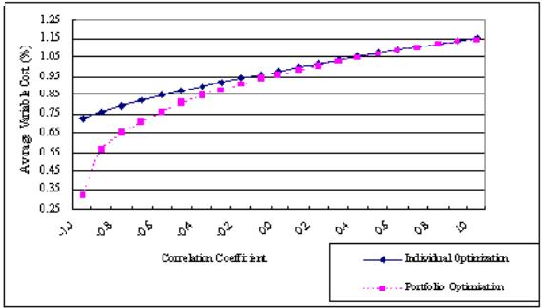
\includegraphics[width=10cm,height=6cm]{fg_b1n.png}
\end{center}
\caption[Correlation coefficient and variable cost in two asset case]{{\bf Correlation coefficient and variable cost in two asset case.}
 \quad This graph shows how variable cost ($y$-axis) changes according to the correlation coefficient
($x$-axis), using market impact coefficients and volatility of typical two stocks.
 Due to diversification effect, simultaneous optimization reduces cost than iterative optimization
($V_1=100$, $V_2=150$, $a_1=0.0002$, $a_2=0.0003$, $\sigma_1=0.001$, $\sigma_2=0.0015$,
$\lambda=1$).}\label{fg_b1}
\end{figure}

%%%%%%%%%%%%%%%%%%%%%%%
\section{Limit to Instantaneous Executable Volume}\label{sec_b4}

\noindent 1) Solution with upper limit 

 So far, we have assumed market impact is linear.  However, in practice, this does not always hold without any restrictions, but only within moderate trading volume and time.  Therefore, in this section, we consider the effect of limit to the volume executable instantaneously.  For simplicity, we study only single asset case.  Without limit, recall that the optimal execution strategy as well as average variable cost have been obtained in Proposition \ref{cor_b1}.

 Now, assume that there is an upper limit $V_0$ to the volume executable instantaneously.  The solution in the above violates the limit when
\begin{equation}\label{eq_b20}
  v(0)=\left( \frac{\lambda^2 \sigma^2 V}{2a^2} \right)^{1/3} > V_0, \qquad
  \mbox{or\ equivalently,} \qquad V>\frac{2a^2V_0^3}{\lambda^2\sigma^2}.
\end{equation}
 If this is the case, it seems difficult to get an explicit form of the optimal solution.  However, since the price movement risk is an increasing function of time while market impact coefficient remains constant, $v(t)$ is considered to be a decreasing function of time.  Therefore, the optimal execution strategy is expected to take a constant value $V_0$ on $[0,t_0]$ and then decrease monotonically to approach zero asymptotically.  Thus, it is natural to approximate the optimal execution strategy as
\begin{equation}\label{eq_b18}
  v_0(t) = \left\{
  \begin{array}{ll}
   V_0, & \quad 0 \leq t < t_0, \\
   V_0 e^{-\beta (t-t_0)}, & \quad t_0 \leq t.
  \end{array}
  \right.
\end{equation}
 From the constraint (\ref{eq_b1}),
\[
  V = \int_0^\infty v_0(t) dt = V_0 \left( t_0 + \frac{1}{\beta} \right)
\]
so that the relation
\begin{equation}\label{eq_b19}
  \beta = \frac{V_0}{V-V_0t_0}
\end{equation}
holds.
 The following proposition identifies optimal $t_0$ (and hence $\beta$) for this approximation.

\begin{proposition}\label{prop_b2}
 \quad Within function class that satisfies (\ref{eq_b18}) and (\ref{eq_b19}),
the optimal $t_0$ is given as a unique solution of
\begin{equation}\label{eq_b30}
  \left(t_0-\gamma\right)^4 + \frac{2a^2V_0^2}{3\lambda^2\sigma^2}
  \left\{ \left( t_0 - \gamma \right)^3-2 \gamma^3 \right\} = 0, \quad
  t_0 \in (0, \gamma);
  \qquad \gamma=\frac{V}{V_0}.
\end{equation}
\end{proposition}
\begin{proof}
  See Section \ref{sec_bappendix}.
\end{proof}

\noindent In order to see the precision of the approximation, we compare the numerical solution and this approximation with real market data.  Figure \ref{fg_b2} shows the optimal execution strategy of stock 1 in the Section \ref{sec_b3}.  The limit to instantaneous execution volume is assumed to be 10 units since the average trading volume was 32 units in that period, and we regard market share over 30\% is too much ($\sigma=0.001$, $a=0.0002$, $\lambda=1$, $V=200$, $V_0=10$).  Figure \ref{fg_b2} supports this approximation.

\begin{figure}[htbp]
\begin{center}
 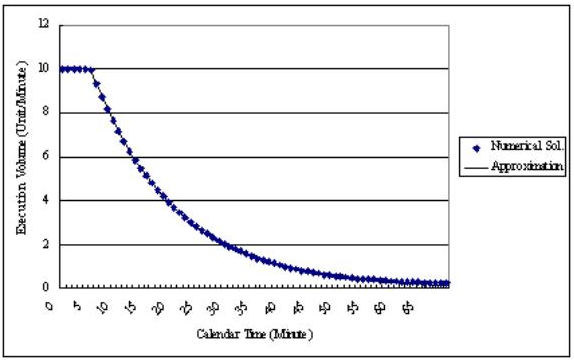
\includegraphics[width=10cm,height=6cm]{fg_b2n.png}
\end{center}
\caption[Numerical solution and approximation for the case with upper limit]{{\bf Numerical solution and approximation for the case with upper limit.}
 \quad Instantaneous execution volume of numerical solution (dashed curve) and approximation (solid curve)
of the optimal execution strategy of the stock in the Section \ref{sec_b3} is on $y$-axis, and time is on $x$-axis.
 The limit to instantaneous execution volume is assumed to be 10.  Approximation is good enough to be
almost indistinguishable with numerical solution.  ($\sigma=0.001$, $a=0.0002$, $\lambda=1$, $V=200$,
$v_0=10$).}\label{fg_b2}
\end{figure}

 For multiple asset case, we can expect an exponential function as we did in the one asset case.  However, the formula of opportunity cost depends on the integration range, and so we need to calculate case by case according to the time when the execution volume of each asset becomes variable.

\bigskip

\noindent 2) Numerical examples

 It is difficult to identify implications on sensitivity of parameters and constraints from the optimal strategies since they require numerical calculation.  So, we study the characteristics of the optimal execution strategy of a single asset case.  Specifically, using parameters of stock 1 in Section \ref{sec_b3}, we observe how average variable cost changes according to whole trading size, and compare each solution.  In this comparison, we also show the behavior of optimal execution strategy in which orders are executed at a constant rate (constant execution henceforth) presented in the following proposition.

\begin{proposition}\label{prop_b3}
 \quad Within constant executions, the optimal execution volume $v_c$ is
\[
  v_c = \left\{
  \begin{array}{ll}
   \left( \frac{\lambda^2 \sigma^2 V}{12a^2} \right)^{1/3},
     & \quad V \leq \frac{12 a^2 V_0^3}{\lambda^2 \sigma^2}, \\
   V_0, & \quad V > \frac{12 a^2 V_0^3}{\lambda^2 \sigma^2}
  \end{array}
  \right.
\]
where, as before, $V_0$ is the upper limit to the volume executable instantaneously.
 In this case, the average variable cost is
\[
  \frac{VC}{V} = \left\{
  \begin{array}{ll}
   \left( \frac{9}{4} a \lambda^2 \sigma^2 V \right)^{1/3},
    & \quad V \leq \frac{12a^2V_0^3}{\lambda^2\sigma^2}, \\
   \left( \frac{\lambda^2\sigma^2V}{3V_0} \right)^{1/2}+aV_0,
    & \quad V > \frac{12a^2V_0^3}{\lambda^2\sigma^2}.
  \end{array}
  \right.
\]
\end{proposition}

\begin{proof}
  See Section \ref{sec_bappendix}.
\end{proof}

\noindent Comparing with Proposition \ref{cor_b1}, the average variable cost under constant execution looks quite similar to that of the general optimal execution strategy (general execution henceforth) for small trading size, but the size is
$(4/3)^{1/3}$ times larger.  Figure \ref{fg_b3} and Figure \ref{fg_b4} show the relationship with whole trading size and average variable cost, using parameters of stock 1 in Section \ref{sec_b3} ($\sigma=0.001$, $a=0.0002$, $\lambda=1$, $V_0=10$).

\begin{figure}[htbp]
\begin{center}
 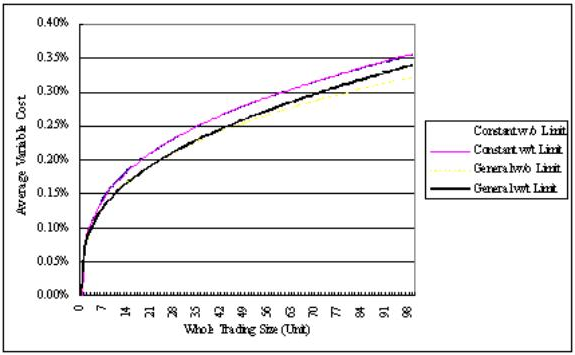
\includegraphics[width=10cm,height=6cm]{fg_b3n.png}
\end{center}
\caption[Whole trading size and average variable cost (small trades)]{{\bf Whole trading size and average variable
cost (small trades).}
 \quad Average variable cost ($y$-axis) is an increasing function of whole trading size ($x$-axis), while the marginal
increment is a decreasing function, which are consistent with intuition.
 Constant execution with limit coincides with constant execution without limit for small trades.
 The same parameters of the stock in Section \ref{sec_b3} are used ($\sigma=0.001$, $a=0.0002$, $\lambda=1$, $V_0=10$).}\label{fg_b3}
\end{figure}

\noindent In Figure \ref{fg_b3}, as long as optimal execution volume is below the limit, average variable costs with and without limit coincide and increase as whole trading size to the power of $1/3$.

\begin{figure}[htbp]
\begin{center}
 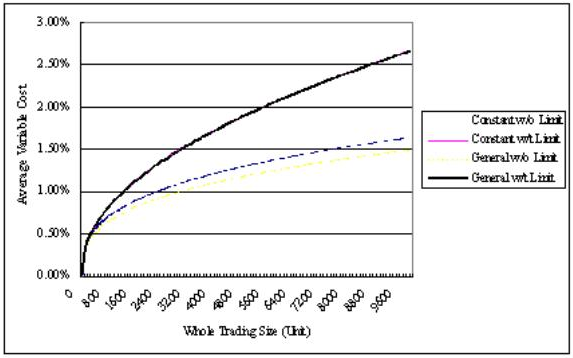
\includegraphics[width=10cm,height=6cm]{fg_b4n.png}
\end{center}
\caption[Whole trading size and average variable cost (large trades)]{{\bf Whole trading size and average variable
cost (large trades).}
 \quad Same graph as Figure \ref{fg_b3}, but for large trades.
 As whole trading size grows, general execution with limit departs from general execution without limit and
approaches constant execution with limit.}\label{fg_b4}
\end{figure}

\noindent As whole trading size grows in Figure \ref{fg_b4}, average variable cost of general execution with limit departs from that of general execution without limit and approaches that of constant execution with limit, which increases as whole trading size to the power of $1/2$.

Further, it is of great interest to compare our optimal execution strategy with those in previous studies such as Almgren and Chriss (1999).  To do so, using parameters on Section 4.4 in Almgren and Chriss (1999), we calculate optimal strategies of both ours and theirs.  They assumed whole trading size $V$ as $10^6$ shares, daily volatility $\sigma$ as $0.95(\$/\mbox{share})/\mbox{day}^{1/2}$, temporary market impact coefficient $a$ as $2.5 \times 10^{-6}(\$/\mbox{share})(\mbox{share}/\mbox{day})$, and risk premium $\lambda$ as $1.645$ for VaR-model and $10^{-6}/\$$ for Variance-model.  Also, the number of time periods was set to five.  We neglect other parameters for simplicity.  Optimal execution strategies are shown in Figure \ref{fg_b5}.  

\begin{figure}[htbp]
\begin{center}
 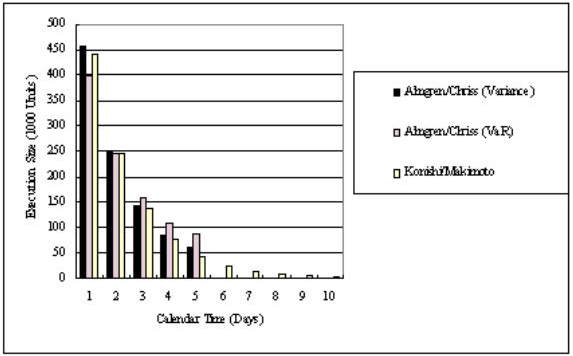
\includegraphics[width=10cm,height=6cm]{fg_b5n.png}
\end{center}
\caption[Comparison of optimal execution strategy.]{{\bf Comparison of optimal execution strategy.}
 \quad Daily execution volume is on $y$-axis, and calendar time is on $x$-axis.
 We can see that, in strategy of Almgren and Chriss (1999), trades which would have best fitted periods after 6 are
somewhat awkwardly pushed into period 3--5 since the number of time
 periods is arbitrarily set to five ($V=10^6$ shares, $\sigma=0.95\mbox{(dollar/share)/day}^{1/2}$, $a=2.5 \times 10^{-6} \mbox{(dollar/share)/day}^{1/2}$, $\lambda =1.645$).}\label{fg_b5}
\end{figure}

\noindent We can see that, in optimal execution strategy of Almgren and Chriss (1999), trades which would have best fitted periods after 6 are somewhat awkwardly pushed into period 3 -- 5 since the number of time periods is arbitrarily set to five.  Further, average variable cost is \$2.18 for our strategy and \$2.60 for that of Almgren and Chriss (1999), and therefore, we can confirm that our model indeed provides lower average cost.

In practice, we suffer statistical errors in estimating parameters.  However, empirical studies such as Uno and Yamada (1993) reports that the market impact coefficients and the price volatilities are rather stable.  Also, it is more realistic to regard parameters stochastic.  However, according to the analysis by Hisata and Yamai (2000) on constant execution, this change does not affect the result significantly.


%%%%%%%%%%%%%%%%%%%%%%%%%
\section{Principle of Optimality}\label{sec_b5}

 In general, optimal policy satisfies the ``principle of optimality," which means that the remaining decision must be the same as the decision taken at the beginning.  However, if we recalculate the optimal execution strategy in Proposition \ref{prop_b1} at halfway, the result differs from the strategy calculated at the beginning.  This is because VaR is not additive regarding time, or standard deviation of price movement is not additive.  This problem might be resolved by introducing a new risk measure although it is often difficult to provide such measure with an exact economical meaning.  For example, standard deviation type measure which ignores historical profit and loss can be defined as
\[
  VC = a \int_0^\infty x'(t)^2 dt + \lambda \sigma \int_0^\infty x(t) dt.
\]
 Here, by Euler's Equation of the calculus of variations,
\[
  -2ax''(t) + \lambda \sigma = 0.
\]
 So, with the initial condition $x(0)=V$,
\[
  v(t) = -x'(t) = \left\{
  \begin{array}{ll}
   - \frac{\lambda \sigma}{2a}t + \sqrt{\frac{\lambda \sigma V}{a}},
     & \quad 0 \leq t < \sqrt{\frac{4aV}{\lambda\sigma}}, \\
   0, & \quad \sqrt{\frac{4aV}{\lambda\sigma}} \leq t.
  \end{array}
  \right.
\]
 We can see that this function satisfies the principle of optimality.
 The average variable cost is,
\[
  \frac{VC}{V} = \frac{4}{3} \sqrt{a \lambda \sigma V}.
\]
 Further, if there is a limit $V_0$ to instantaneous execution volume,
\[
  v(t) = \left\{
  \begin{array}{ll}
   V_0, & \quad 0 \leq t < \frac{V}{V_0}-\frac{aV_0}{\lambda \sigma}, \\
   -\frac{\lambda\sigma}{2a}t + \frac{\lambda\sigma V}{2aV_0} + \frac{V_0}{2},
       & \quad \frac{V}{V_0}-\frac{aV_0}{\lambda \sigma} \leq t < \frac{V}{V_0}+
         \frac{aV_0}{\lambda \sigma}, \\
   0, & \quad  \frac{V}{V_0}+\frac{aV_0}{\lambda \sigma} \leq t
  \end{array}
  \right.
\]
and
\[
  \frac{VC}{V} = \frac{\lambda\sigma V}{2V_0} + aV_0 - \frac{a^2V_0^3}{6\lambda\sigma V}.
\]
 This value increases almost linearly as $V$ increases, which still contradicts the empirical results
of BARRA (1997) and Mannen and Uno (2000).

%%%%%%%%%%%%%%%%%%%%
\section{Closing Remarks}\label{sec_b6}

This chapter has studied execution scheduling of liquidation of a block trade and formulated it as a static optimization problem.  Based on empirical studies on market microstructure, we have distinguished between temporary market impact and permanent market impact, and assumed that each component to be a linear function of trading volume within moderate volume and time.  Also, we have defined the measure of opportunity cost as standard deviation of price movement, and minimized transaction cost, sum of execution cost and opportunity cost.  Under this framework, we have obtained explicit solutions both for the single-asset case and a multiple-asset portfolio model in the form of pure exponentials.  Further, we have derived an approximation formula when there is a limit to the trading volume
executable instantaneously.  

As a result, we have shown that the optimal execution strategy is independent of permanent impact, that optimal execution duration is an increasing function of whole trading size, and that the optimal average cost is an increasing function of whole trading size, price volatility, and temporary impact, and a decreasing function of the limit to instantaneous execution volume, which are all consistent with trading practice and empirical studies.  Specifically, optimal average cost increases as whole trading size to the power of $1/3$ for small orders and $1/2$ for large orders.  Further, it is shown that the transaction cost can be lowered by making order execution late when price movement risk of a portfolio is well diversified.

Our results are immediately applicable to existing risk management framework and provides explicit solution for minimum L-VaR.  Also, although this chapter uses an example of liquidation of a block of common stock, results can be extended over wider problems on liquidation of any large block of assets.

 While this chapter has focused on static optimization, decision change in accordance with new information might be handled by dynamic programming.  Also, this model can reflect more reality by making volatility and market impact time dependent.  Further, it is an interesting issue how to relate order slicing strategy and choice between market order and limit order, and how to control information effect of orders.  These issues are left for further analysis.

\bigskip
\bigskip




%%%%%%%%%%%%%%%%%%%%%%%%
\section{Appendix}\label{sec_bappendix}
\subsection{Proof of Lemma \ref{lem_b3}}
Since $\S$ is non-negative definite, $E \geq 0$ is clear.  Thus, it is enough to prove $EG \geq F^2$.  Non-negative definiteness of $\S$ also implies each eigenvalue $\xi_i\ (i=1,\cdots,N)$ of $\S$ is non-negative (c.f., Bellman (1997), Ch.4.8, Theorem 3).
 This and symmetricity of $\S$ ensure the existence of an orthogonal matrix $\H$ for which
$\S = \H \mbox{Diag}(\xi_1,\cdots,\xi_N) \H^\top$ holds.
 Therefore, if we define $\Q = \H \sqrt{\J} \H^\top$ with $\sqrt{\J} = \mbox{Diag}(\sqrt{\xi_1},\cdots,
\sqrt{\xi_N})$, then $\Q$ is symmetric and $\Q^2=\S$.
 Let $\u(t) = \Q \x(t)$ and $\w(t) = \Q \y(t)$.
 Then, we get
\[
  \x(t)^\top \S \x(t) = \u(t)^\top \u(t), \qquad
  \y(t)^\top \S \y(t) = \w(t)^\top \w(t), \qquad
  \x(t)^\top \S \y(t) = \u(t)^\top \w(t).
\]
 By Cauchy-Schwartz's inequality (cf., Kolmogorov and Fomin (1970)),
%\begin{equation}\label{eq_b11}
%  \x(t)^\top \S \x(t) \cdot \y(t)^\top \S \y(t) \geq [ \x(t)^\top \S \y(t) ]^2.
%\end{equation}
% Since both $\x(t)^\top \S \x(t)$ and $\y(t)^\top \S \y(t)$ are non-negative,
%(\ref{eq_b11}) implies
%\[ %begin{equation}\label{eq_b12}
%  \sqrt{\x(t)^\top \S \x(t)} \cdot \sqrt{\y(t)^\top \S \y(t)} \geq
%  | \x(t)^\top \S \y(t) |
%\] %\end{equation}
%which together with Schwartz's integral inequality show
\begin{eqnarray*}
  \left( \int_0^\infty \x(t)^\top \S \x(t) dt \right)
  \left( \int_0^\infty \y(t)^\top \S \y(t) dt \right)
  & = & 
   \left( \int_0^\infty \u(t)^\top \u(t) dt \right)
   \left( \int_0^\infty \w(t)^\top \w(t) dt \right) \\
  & \geq & \left( \int_0^\infty \u(t)^\top \w(t) dt \right)^2 \\
  & = & \left( \int_0^\infty \x(t)^\top \S \y(t) dt \right)^2,
\end{eqnarray*}
completing the proof.


\subsection{Proof of Proposition \ref{prop_b2}}
 For notational simplicity, we calculate $VC/V_0^2$ instead of $VC$.
 Let $\gamma = V/V_0$.
 Then, from (\ref{eq_b18}) and (\ref{eq_b19}),
\[
  \int_0^\infty \frac{v_0(t)^2}{V_0^2} dt = 
  \left[ \int_0^{t_0} dt + \int_{t_0}^\infty e^{-2\beta(t-t_0)} dt \right]
  = \frac{t_0+\gamma}{2}.
\]
 Further, if we let $x_0(t) = \int_t^\infty v_0(s) ds$,
\[
  \frac{x_0(t)}{V_0}
   = \left\{
   \begin{array}{ll}
    \gamma - t, & \quad 0 \leq t < t_0, \\
    \beta^{-1} e^{-\beta(t-t_0)}, & \quad t_0 \leq t.
   \end{array}
   \right.
\]
 So,
\[
  \int_0^\infty \frac{x_0(t)^2}{V_0^2} dt
   = \int_0^{t_0} (t-\gamma)^2 dt + \int_{t_0}^\infty \beta^{-2}
     e^{-2\beta (t-t_0)} dt
   = -\frac{1}{6} (t_0 - \gamma)^3 + \frac{1}{3} \gamma^3.
\]
 Therefore,
\begin{equation}\label{eq_b31}
  \frac{VC}{V_0^2} = \frac{a(t_0+\gamma)}{2} + \frac{\lambda \sigma}{\sqrt{6}\,V_0}
  \sqrt{-(t_0-\gamma)^3+2\gamma^3} =: f(t_0).
\end{equation}
 Note that the range of $f(t_0)$ is $t_0 \in (0,\gamma)$ from (\ref{eq_b18}).
 Since the first term of $f(t_0)$ linearly increases as $t_0$ increases while the second
term is a convex decreasing function, $f(t_0)$ is convex.
 Moreover,
\[
  f'(t_0) = \frac{1}{4} \left\{ 2a - \frac{\lambda \sigma}{\sqrt{6} \, V_0}
  \frac{(t_0-\gamma)^2}{\sqrt{-(t_0-\gamma)^3+2\gamma^3}} \right\}.
\]
 Then,
\begin{eqnarray*}
  & & f'(0) = \frac{1}{4} \left( 2a - \frac{\sqrt{2\gamma}\lambda\sigma}{V_0} \right) < 0, \qquad
              \mbox{(from (\ref{eq_b20}))} \\
  & & f'(\gamma) = \frac{a}{2} > 0.
\end{eqnarray*}
 Summarizing these arguments, we conclude that $t_0$ that minimizes $VC/V_0^2$ is given
as a unique solution of $f'(t_0)=0$, $t_0 \in (0,\gamma)$.
 Rearranging terms, the desired result is obtained.

%%%%%%%%%%%%%%%
\subsection{Proof of Proposition \ref{prop_b3}}
 Consider a constant execution in which orders are executed at a constant volume $v_c$ until time $t_0$.
 According to the constraint in (\ref{eq_b1}), $v_c$ and $t_0$ satisfy
\begin{equation}\label{eq_b32}
  \int_0^{t_0} v_c dt = v_c t_0 = V, \qquad \mbox{or} \qquad v_c = \frac{V}{t_0}.
\end{equation}
 Noting that
\[
  x(t) = \left\{
  \begin{array}{ll}
   (t_0-t)v_c, & \quad 0\leq t\leq t_0, \\
   0, & \quad t_0 < t,
  \end{array}
  \right.
\]
the total cost can be calculated as
\[
  VC = a \frac{V^2}{t_0} + \lambda \sigma V \sqrt{\frac{t_0}{3}}.
\]
 Therefore, the optimal $t_0$ that minimized the variable cost is
\[
  t_0 = \left( \frac{12a^2V^2}{\lambda^2\sigma^2} \right)^{1/3},
\]
and, from (\ref{eq_b32}), the optimal execution volume is
\[
  v_c = \left( \frac{\lambda^2 \sigma^2 V}{12a^2} \right)^{1/3}.
\]
 Also, average variable cost becomes
\[
  \frac{VC}{V} = \left( \frac{9}{4} \lambda^2 \sigma^2 aV \right)^{1/3}.
\]
 When there is a limit $V_0$ to instantaneous execution volume, $t_0$ needs to satisfy
$t_0 \geq V/V_0$.
 In summary, the optimal execution period is given as
\[
  t_0 = \max \left( \left( \frac{12a^2V^2}{\lambda^2\sigma^2} \right)^{1/3}, \frac{V}{V_0} \right)
\]
and the desired results can be obtained by a straightforward calculation.

% 02/01 changed according to ref No.2
% 02/05 changed from .emf to n.png
% 03/07 Changed as the mail on 02/02/28

%%%%%%%%%%%%%%%
% Limit Order%%
%%%%%%%%%%%%%%%

%\setcounter{section}{0}

\chapter{Selection of Market and Limit Order}\label{chap_l}


%%%%% local definition
\def\va{v_{1a}-\frac{p_1}{a_1}}
\def\vm{v_{1m}-\frac{p_1}{a_1}}
%\def\vl{v_{1l}-\frac{p_1}{a_1}}
%\def\vld{v_{1l}'-\frac{p_1}{a_1}}
%\def\vldd{v_{1l}''-\frac{p_1}{a_1}}
%\def\pa{\frac{p_1}{a_1}}

\def\v1{v_1-\frac{p_1}{a_1}}
\def\u1{u_1-\frac{p_1}{a_1}}
%\def\vl{v_{1l}-\frac{p_1}{a_1}}
\def\pa{\frac{p_1}{a_1}}

\def\px{\phi_x}
\def\Px{\Phi_x}
\def\pmx{\phi_{-x}}
\def\Pmx{\Phi_{-x}}
\def\py{\phi_y}
\def\Py{\Phi_y}
\def\pmy{\phi_{-y}}
\def\Pmy{\Phi_{-y}}
\def\gx{G_x}
\def\gmx{G_{-x}}
\def\gy{G_y}
\def\gmy{G_{-y}}
\def\p0{\phi_0}
\def\sgn{\mbox{sgn}}


%%%%%%%%%%%%%%%%%%%%%


\begin{quote}
{\bf Abstract} \quad This chapter analyses the optimal selection of market and limit orders in a series of single price batch auctions when the expectation of the limit order book is given.  We derive the analytical solution of a single limit order model for risk neutral traders, and then extend the result for risk averse traders.  We find that the limit order size is independent of the whole trade size while the limit order price and the market order size are linear functions and that market orders replace limit orders as time passes.  Further, we calculate economic value of monitoring limit order book.

\end{quote}

%%%%%%%%%%%%%%%
\section{Introduction}\label{sec_l1}
Market and limit orders are two essential instruments of order placement.  Progress in information technology has improved order processing capability and made order placement strategy a critical issue in investment.  For example, order driven markets such as the Tokyo Stock Exchange (TSE) have excluded floor traders and adopted an automatic matching system, which makes order processing faster and more certain.  Also, several markets such as the New York Stock Exchange (NYSE) and the National Association of Securities Dealers Automated Quotation System (NASDAQ) start receiving limit orders to broaden traders' freehand for order placement.  Further, emergence of alternative trading systems such as crossing networks and electronic communication networks enables traders to tactically submit and cancel orders across markets.  In practice, traders recognize the advantage of limit orders: cost efficiency, and disadvantages: uncertain execution and free option, and choose either market or limit order or sometimes both as fits their objectives and circumstances.  

Several empirical studies confirm traders' behavior in the real market.  For example, Biais et al. (1995) analyzed trading data from the Paris Stock Exchange and find that traders actively respond to public orders (orders submitted by other traders).  Specifically, market orders are preferred when bid-ask spread is small because the execution probability of limit order is low, while limit orders are preferred when bid-ask spread is large.  Also, Harris and Hasbrouck (1996) analyzed data from NYSE and found that 60\% of limit orders which lay inside the best bid and ask prices were executed.  They show that the trading cost can be lowered by limit orders especially when bid-ask spread is large, which is consistent with the result of Biais et al. (1995).  Regarding Japanese market, Kawahara (1994) analyzes TSE stock data in 1994 and finds that trading cost with limit orders is 0.15\% lower than that with only market orders.  Also, trading cost turns out to be larger for sell orders, large orders, and limit orders that are exposed to the market at shorter period of time.

In contrast, theoretical studies are limited for the selection of market
and limit orders.  For example, although Bertisimas and Lo (1998) and Konishi and Makimoto (2001) derive the optimal order slicing strategy in a large portfolio liquidation, only market orders but no limit orders are allowed in their models.  Also, Parlour (1999) analyses how market conditions affect the selection of market and limit orders when a trader places just one unit of order.  This analysis shows the interaction between trader's order placing strategy and market conditions, but fails to study how traders split orders for large trades.  Further, Chakravarty and Holden (1995) provide a theoretical model which explains how traders select market and limit orders in a quote driven market.  However, existence of a market maker is crucial in their model, and the results are not directly applicable to an order driven market.

Accordingly, this chapter analyzes the optimal selection of market and
limit orders, sizes, prices, and times in a series of single price batch
auctions.  Specifically, we derive the analytical solution of a single
limit order model for risk neutral traders, and then extend the result
for risk averse traders.  Regarding the execution at each period, we
find that the optimal limit order size is independent of the whole trade
size so as to balance the non-linearity of execution volume and price.
In contrast, the limit order price and the market order size are linear
functions in order to balance trading costs across trading periods.
Regarding the execution throughout the trading session, market orders
replace limit orders as time passes, and necessity of completing
execution grows.  Further, if trading volume and price volatility are
larger at the opening and closing of the trading session as in the
practical markets, more limit orders are tried at the opening and
closing.  These results are consistent with intuitive trading behaviors.
Further, although most traders know the public order book as
expectations as in our model, member security brokers are allowed to
monitor the public order book without time lags.  So, we evaluate the
value of monitoring public order books and provide criteria for
selecting stocks to monitor.

The rest of this chapter is organized as follows.  First, by dynamic programming, Section \ref{sec_l2} derives the analytical solution of a single limit order model for risk neutral traders.  Then, Section \ref{sec_l3} shows several variations of the model in Section \ref{sec_l2} for risk averse traders and when public market orders are known.  Further, Section \ref{sec_l4} analyzes a numerical solution of a multiple limit order model.  Finally, section \ref{sec_l5} concludes the analysis.

%%%%%%%%%%%%%%%%%
\section{Standard Single Limit Order Model}\label{sec_l2}
\subsection{Formulization of the Strategy}
Imagine a case in which a trader buys a certain number of shares $R_1$ in a series of $T$ single price batch auctions.  The trader tries to minimize the expected value of the purchase price with market and limit orders.  We assume that the trader has just the expectation of the public limit orders and knows the distribution of the public market orders but not concrete order sizes since it is costly or prohibited for most traders to monitor public order books.   Lehman and Modest (1994) find that stocks with low liquidity tend to be traded at {\it Itayose}, single price batch auctions at the opening and the closing of the trading sessions on the TSE.  Although our model is applicable to any stock it has a better fit with low liquidity stocks.  We make the following assumptions about market environments, which are given exogenously.

\begin{assumption}\label{ass_l1}
\quad
\begin{enumerate}
\item Price change is driven by two uncertainties, change of fundamental value, $Q_i$, and size of public market orders, $M_i$.  $Q_i$ is given as 
\[ %begin{equation}\label{eq_l1}
   Q_i = Q_1 + \sum_{j=2}^i \delta_j \epsilon_j
\] %end{equation}
where $Q_1$ and $\delta_j\ (j=2,\cdots,T)$ are constants and
      $\epsilon_j\ (j=2,\cdots,T)$ are serially uncorrelated random
      variables that follow N(0,1).  $M_i$ are serially uncorrelated
      random variables that follow $\mbox{N}(0,\sigma_i^2)$ and are
      independent of $\epsilon_i\ (i=2,\cdots,T)$ also.
\item Market impact at the $i^{th}$ period $P_i$ is a linear function of execution volume with a constant market impact coefficient $a_i$, and $r \ (0 \leq r \leq 1)$ of market impact is passed to subsequent periods as the permanent impact.
\end{enumerate}
\end{assumption}

Regarding the price change, a positive (negative) number of $M_i$ represents a buy (sell) market order, respectively.  The assumption that $M_i$ is serially uncorrelated and independent of $Q_i$ is natural since market orders by the uninformed liquidity traders tend to be numerous and small, and therefore, excess market orders follow independent normal distribution by the Central Limit Theorem.

Regarding market impact, we can justify the linear function assumption both empirically and theoretically.  From the empirical point of view, Jain and Joh (1988) and Holthausen et al.~(1987) observe that the market impacts are rather stable linear functions and can be divided into temporary and permanent components.  From the theoretical point of view, linear market impact is realized when informed traders submit limit orders while uninformed liquidity traders submit market orders.  Specifically, assume that risk averse informed traders try to take advantage of temporary market impact as contrarians and submit limit orders.  Let $\lambda$ denote traders' risk premium, $P$ execution price, and $V$ execution size, and the traders' objective function can be written as
\[ %begin{equation}\label{eq_l2}
  U = (1-r) P V - \lambda V^2
\] %end{equation}
where $r$ is the temporary market impact ratio as defined in Assumption \ref{ass_l1}.

So, the optimal position size $\ol{V}$ satisfies
\[ %begin{equation}\label{eq_l3}
  \left. \pdif{U}{V} \right|_{V=\ol{V}}= (1-r) P - 2 \lambda \ol{V} = 0.
\] %end{equation}
And therefore,
\[ %begin{equation}\label{eq_l4}
  \ol{V} = \frac{(1-r) P}{2 \lambda}.
\] %end{equation}
This is attained by submitting limit orders with equal size for any prices, since
\[ %begin{equation}\label{eq_l5}
  \pdif{\ol{V}}{P} = \frac{(1-r)}{2 \lambda}.
\] %end{equation}
Further, Bertisimas and Lo's (1998) analysis on optimal execution
without limit orders assumes linear market impact and randomness with
normal distribution.  Therefore, we can evaluate economical value of
limit orders by comparing with our results and those of Bertisimas and Lo (1998).

In a single price batch auction, market orders, buy limit orders at higher prices than the execution price, and sell limit orders at lower prices than the execution price are executed.  Market impact $P_1$ is determined so as to balance total buy orders and sell orders.  Therefore, linear market impact is realized by public limit orders.  Specifically, $\displaystyle Q_i+r \sum_{j=1}^{i-1}P_j$ is passed to the subsequent periods since the ratio of permanent impact is $r$.  Therefore, we define base price at the $i^{th}$ period as
\begin{equation}\label{eq_l6}
  B_i = \left\{
  \begin{array}{ll}
    Q_1, \quad & i=1, \\
    \displaystyle Q_i+ r \sum_{j=1}^{i-1} P_j, & i=2,\cdots,T.
  \end{array}
  \right.
\end{equation}
Since market impact coefficient in the $i^{th}$  period is $a_i$, $1/a_i$ of public sell limit orders exist at any prices above $B_i$, and $1/a_i$ of public buy limit orders exist at any prices below $B_i$.  

Regarding the trader's strategy, we assume that the trader knows constant parameters and $Q_i$ but not $M_i$ when he decides the $i^{th}$ period strategy.  Also, we assume that the trader can submit only one market and limit order for simplicity.  As a result, our model has three controllable variables: the trader's market order size $u_i$, sum of the trader's market and limit order sizes $v_i$, and deviation of limit order price from the base price $p_i$, which we call a base limit order price.  Note that the limit order size is given by $w_i \define v_i-u_i$ and that actual limit order price is $B_i+p_i$.  We allow $u_i$ and $p_i$ to take negative values while the size of limit order $w_i$ must not be negative because negative $w_i$ is just a cancellation of a buy limit order but not equivalent with a sell limit order.  Instead, without loss of generality, we can regard limit order as ``buy" because a sell limit order can be synthesized by a combination of a sell market order and a buy limit order.  Note that all the remaining orders at the last period are submitted as market orders in order to complete the execution.  These assumptions are summarized as follows.

\begin{assumption}\label{ass_l2}
 \quad Execution strategy is specified as $\mbpsi = \{ \psi_i ; i=1,\cdots,T \}$ where $\psi_i = (u_i, v_i, p_i)$, and satisfies the following conditions.
 \begin{enumerate}
  \item $u_i \leq v_i\ (i=1,\cdots,T)$.
  \item $\psi_i$ is $\calG_i$-measurable where $\calG_i = \sigma \{ \epsilon_2, \cdots, \epsilon_i, M_1, \cdots, M_{i-1} \}$, the smallest $\sigma$-algebra with respect to which $\epsilon_2, \cdots, \epsilon_i$ and $M_1, \cdots, M_{i-1}$ are measurable.
  \item Only market order is allowed at the $T^{th}$ period.
 \end{enumerate}
\end{assumption}

Once $\psi_i$ is chosen and $M_i$ is realized, the execution price $B_i+P_i$ and the execution volume $D_i$ are determined uniquely as a function $P_i=\pi_i(u_i,v_i,p_i,M_i)$ and $D_i=\kappa_i(u_i,v_i,p_i,M_i)$.  Specifically, if $p_i > 0$, since volume of public sell limit orders below $B_i+p_i$ is $p_i/a_i$, trader's limit order starts being executed when the sum of public and the trader's market order (the total market order henceforth) is smaller than $p_i/a_i$, and is completely executed when the total market order is smaller than $-w_i+p_i/a_i$.  Next, if $p_i \leq 0$, since volume of public buy limit orders above $B_i+p_i$ is $-p_i/a_i$, trader's limit order starts being executed when the total market order is smaller than $p_i/a_i$, and is completely executed when the total market order is smaller than $-w_i+p_i/a_i$.  Consequently, 
\begin{equation}\label{eq_l7}
  \kappa_i(u,v,p,m) = \left\{
  \begin{array}{ll}
   u, \quad & -u + p/a_i < m, \\
   -m+p/a_i, & -v+p/a_i < m \leq -u + p/a_i, \\
   v, & m \leq -v + p/a_i.
  \end{array}
  \right.
\end{equation}
Similar arguments show that 
\begin{equation}\label{eq_l8}
  \pi_i(u,v,p,m) = \left\{
  \begin{array}{ll}
   a_i(u+m), \quad & -u + p/a_i < m, \\
   p, & -v+p/a_i < m \leq -u + p/a_i, \\
   a_i(v+m), & m \leq -v + p/a_i.
  \end{array}
  \right.
\end{equation}
If there are no limit orders, we define $u_i=v_i$, $p_i=-\infty$.

There are two non-linearities in (\ref{eq_l7}) and (\ref{eq_l8}).  The first is the non-linearity of execution volume since limit orders are not executed when the execution price is higher than the limit order price.  The advantage of non-linearity of execution volume is more significant for larger limit orders.  The second non-linearity is that of execution price.  Execution price becomes higher because of the trader's limit order, which makes the execution price like a ``vertical spread", combination of buy and sell of put options.  The disadvantage of non-linearity of execution price is more significant for larger limit orders.  Therefore, it is expected that the optimal limit order size balances these two non-linearities.

In summary of Assumptions \ref{ass_l1} and \ref{ass_l2}, the execution at the $i^{th}$ period proceeds as follows:
\begin{enumerate}
\item Base price $B_i$ is given by (\ref{eq_l6}).
\item $1/a_i$ of public sell limit orders are submitted at any prices above $B_i$, and public buy limit orders below $B_i$.  
\item The trader selects $u_i$, $v_i$, and $B_i+p_i$.
\item Volume of the public market order $m_i=M_i$ is realized according to $\mbox{N}(0,\sigma_i^2)$, and the execution price and the execution volume is set to $B_i+P_i$ and $D_i$ by (\ref{eq_l7}) and (\ref{eq_l8}), respectively.
\end{enumerate}

Let $\displaystyle R_i \define \sum_{j=i}^T D_j = R_1 - \sum_{j=1}^{i-1} D_j$ denote the size of trades left at the $i^{th}$ period.  Then, the total purchase cost is given as
\begin{eqnarray*}
  \mbox{(Total Cost)}
   & = & \sum_{i=1}^T \left( Q_i + r \sum_{j=1}^{i-1} P_j + P_i \right) D_i \nonumber \\
   & = & \sum_{i=1}^T \left( Q_1 + \sum_{j=2}^i \delta_j \epsilon_j + r \sum_{j=1}^{i-1} P_j + P_i \right) D_i \nonumber \\
   & = & Q_1 \sum_{i=1}^T D_i + \sum_{i=2}^T \sum_{j=2}^i \delta_j \epsilon_j D_i + r \sum_{i=1}^T \sum_{j=1}^{i-1} P_j D_i + \sum_{i=1}^T P_i D_i \nonumber \\
   & = & Q_1 R_1 + \sum_{j=2}^T \delta_j \epsilon_j \sum_{i=j}^T D_i + r \sum_{j=1}^{T-1} P_j \sum_{i=j+1}^{T} D_i + \sum_{i=1}^T P_i D_i \nonumber \\
   & = & Q_1 R_1 + \sum_{j=2}^T \delta_j \epsilon_j R_j + \sum_{i=1}^{T-1} r P_i (R_i-D_i) + \sum_{i=1}^T P_i D_i \nonumber \\
   & = & Q_1 R_1 + \sum_{j=2}^T \delta_j \epsilon_j R_j + \sum_{i=1}^T P_i \{(1-r) D_i +r R_i\}. \label{eq_l9}
\end{eqnarray*}
If we define $\calF_i \define \sigma \{ \epsilon_2, \cdots, \epsilon_i, M_1, \cdots, M_i \}$, $R_j$ is $\calF_{j-1}$-measurable by Assumption \ref{ass_l2}.  Since $\epsilon_j$ and $R_j$ are independent, the expected total purchase cost is 
\[ %begin{equation}\label{eq_l10}
 \ex{\mbox{(Total Cost)}}= Q_1 R_1 + \sum_{i=1}^T \ex{P_i \{(1-r) D_i +r R_i\}}.
\] %end{equation}
Therefore, our problem can be written as
\begin{equation}\label{eq_l11}
  \mbox{minimize} \quad \sum_{i=1}^T \ex{P_i \{(1-r) D_i +r R_i\}}.
\end{equation}  
Define the cost at the $i^{th}$ period as
\[ %begin{equation}\label{eq_l12}
  \ex{P_i \{(1-r) D_i +r R_i\}} = \ex{\pi_i(\psi_i,M_i) \{(1-r) \kappa_i(\psi_i,M_i) +r R_i\}}
\] %end{equation}
where $\psi_i=(u_i,v_i,p_i)$, and $\pi_i(\psi_i,m)$ and $\kappa_i(\psi_i,m)$ stand for $\pi_i(u_i,v_i,p_i,m_i)$ and $\kappa_i(u_i,v_i,p_i,m_i)$ respectively for the simplicity of representaion.

Note that the accumulated market impact $\displaystyle r \sum_{j=1}^{i-1} P_j$ is recognized as the cost at the $j^{th}$ period but not at the $i^{th}$ period.  Since $\epsilon_i\ (i=2,\cdots,T)$, $M_i\ (i=1,\cdots,T)$ are serially uncorrelated and independent with each other, execution strategy at the $i^{th}$ period affects the cost after the $i+1^{th}$ period only through $R_{i+1}$.  Therefore, in order to search for an optimal execution strategy, all we have to consider is Markov policies in which $\psi_i$ is determined solely by $R_i$.  

Specifically, (\ref{eq_l11}) is the Markov decision process whose state is represented by $R_i\ (i=1,\cdots,T)$.  The order selection rule is described by the policy $\psi_i = (u_i, v_i, p_i)$.  Once $R_i$ and $\psi_i$ are given, the state at the $i+1^{th}$ period is $R_i-\kappa_i(\psi_i,m)$ with transition density ${\displaystyle f_i(m)=\frac{1}{\sqrt{2\pi}\sigma_i} \mbox{exp} (-m^2/2\sigma_i^2)}$.  Let the superscript $*$ denote the optimal solution henceforth.  Then, the optimal cost after the $i^{th}$ period with $R_i$ is
\begin{equation}\label{eq_l13}
  C_i^*(R_i) = \min_{\mbpsi} \sum_{j=i}^T \cex{P_j \{(1-r) D_j +r R_j\}}{R_i},
\end{equation}
where $\mbpsi$ denotes the policy space.
Bellman Equation for $i=1,\cdots,T-1$ is given as
\begin{eqnarray}
  C_i^*(R_i)
   & = & \min_{\psi_i} \ex{ \pi_i(\psi_i,M_i) \{(1-r) \kappa_i(\psi_i,M_i) + r R_i \}+ C_{i+1}^*(R_i-\kappa_i(\psi_i,M_i))} \nonumber \\
   & = & \min_{\psi_i} \int_{-\infty}^\infty
         \left[ \pi_i(\psi_i,m) \{(1-r) \kappa_i(\psi_i,m) + r R_i \}+ C_{i+1}^*(R_i-\kappa_i(\psi_i,m)) \right] f_i(m) dm. \label{eq_l14}
\end{eqnarray}
Since only market order is allowed at the $T^{th}$ period, $C_T^*(R_T)$ can be calculated explicitly as
\begin{equation}\label{eq_l18}
  C_T^*(R_T)=a_T R_T^2.
\end{equation}
  Solving (\ref{eq_l14}) backward with the initial condition (\ref{eq_l18}), we can derive the optimal execution strategy at each period.

%%%%%%%%%%%%%%%%%%%%%
\subsection{Derivation of the Optimal Strategy}
We first consider two period case, and then extend it to multiple period case in Section \ref{sec_l23} by Markov decision process.  In order to complete the execution, all the remaining orders are submitted as market orders in the second period.  In this case, since $\cex{P_2}{R_2}=a_2 R_2$, \[ %begin{equation}\label{eq_l15}
  C_1 (R_1)=  \ex{P_1 \{(1-r) D_1 +r R_1\}+a_2(R_1-D_1)^2}.
\] %end{equation}
Further calculation shows the following proposition.
\begin{proposition}\label{prop_l1}
\begin{eqnarray*}
  C_1(R_1) & = &  \{(1-r)a_1+a_2\}v_{01}^2+(ra_1-2a_2)R_1v_{01}+a_2R_1^2 \nonumber \\
      &   &  - [\{(1-r)a_1+a_2\}(u_1+\frac{p_1}{a_1})+(ra_1-2a_2)R_1]\{(\u1)\Phi(-\frac{1}{\sigma_1}(\u1))-\sigma_1 \phi(-\frac{1}{\sigma_1}(\u1))\} \nonumber \\
      &   &  + [\{(1-r)a_1+a_2\}(v_1+\frac{p_1}{a_1})+(ra_1-2a_2)R_1]\{(\v1)\Phi(-\frac{1}{\sigma_1}(\v1))-\sigma_1\phi(-\frac{1}{\sigma_1}(\v1))\} \nonumber \\
      &   &  +a_2\sigma_1^2 \{\Phi(-\frac{1}{\sigma_1}(\u1))-\Phi(-\frac{1}{\sigma_1}(\v1))\} \label{eq_l16}
\end{eqnarray*}
where $\displaystyle \phi(x)=\frac{1}{\sqrt{2\pi}}exp(-\frac{x^2}{2})$ and $\Phi(x)= \int_{-\infty}^x \phi(y) dy.$
\end{proposition}

\begin{proof}
  See Section \ref{sec_lappendix}.
\end{proof}

\noindent Further, the following proposition holds for the corresponding optimal solution.

\begin{proposition}\label{prop_l2}
 \quad Optimal $u_1^*$, $w_1^*$, and $p_1^*$ are uniquely determined to satisfy
\begin{equation}\label{eq_l17}
 \left\{
  \begin{array}{ll}
   \displaystyle p_1^* = -\frac{(ra_1-2a_2)a_1R_1}{2\{(1-r)a_1+a_2\}}, \\
   \displaystyle \frac{w_1^*}{2\sigma_1}= \frac{(1-r)a_1}{2\{(1-r)a_1+a_2\}}\frac{\phi(\frac{w_1^*}{2\sigma_1})}{\Phi(-\frac{w_1^*}{2\sigma_1})},\\
   \displaystyle u_1^*= \frac{p_1^*}{a_1} - \frac{w_1^*}{2}. \\
  \end{array}
  \right.
\end{equation}
\end{proposition}
\begin{proof}
  See Section \ref{sec_lappendix}.
\end{proof}
\begin{remark}
 \quad The second equation in (\ref{eq_l17}) has a unique solution $w_1^*$.
 See Section \ref{sec_lappendix} for detail.
\end{remark}

The first equation in (\ref{eq_l17}) states that the base limit order price is chosen at the peak of the distribution of market order.  This is because the value of the non-linearity of execution volume is maximum at the peak of the distribution.  Besides, $\displaystyle \frac{w_1^*}{2\sigma_1}$ is a constant which depends only on $a_1$, $a_2$, and $r$.  This is because a trader should not place large limit orders due to the non-linearity of execution price.  Further, $u_1^*$, $v_1^*$, and $p_1^*$ are linear functions of $R_1$.

Minimal $C_1^*(R_1)$ is given by
\[ %begin{equation}\label{eq_l18}
  C_1^*(R_1) = \frac{\{4a_2-r^2a_1\}a_1}{4\{(1-r)a_1+a_2\}}R_1^2 - \frac{\{(1-r)a_1+2a_2\}(1-r)a_1\sigma_1^2\phi^2(\frac{w_1^*}{2\sigma_1})}{2\{(1-r)a_1+a_2\}\Phi(-\frac{w_1^*}{2\sigma_1})} + a_2\sigma_1^2\{2\Phi(\frac{w_1^*}{2\sigma_1})-1\}.
\] %end{equation}
Minimal cost is a sum of the square of $R_1$ and a constant because the second and third term do not depend on $R_1$.  Besides, the first term is equal to the minimal cost without limit orders.  Therefore, the difference, sum of the second and third term, is the economical value of limit orders, which is negative and independent of $R_1$.  

It seems that even if $R_1$ is zero, positive expected return can be made by placing small buy and sell limit order at price zero.  This is partly because we ignore bid-ask spread, which makes market impact in the second period negligible.  This approximation error might be significant if the trade is too small.

If sell orders are not allowed, all we have to do is to replace negative value of $u_1^*$ and $v_1^*$ with zero because of the positive second order condition of optimality.  Figures \ref{fg_l1} and \ref{fg_l2} show the relationship between trade size and $u_1^*$, $w_1^*$, and $p_1^*$ for both with and without non-negative constraints when $a_1=a_2=1$, $\sigma_1=10$, and $r=0$.  We can see that limit orders are preferred in small trades even when sell orders are not allowed.

\begin{figure}[htbp]
\begin{center}
 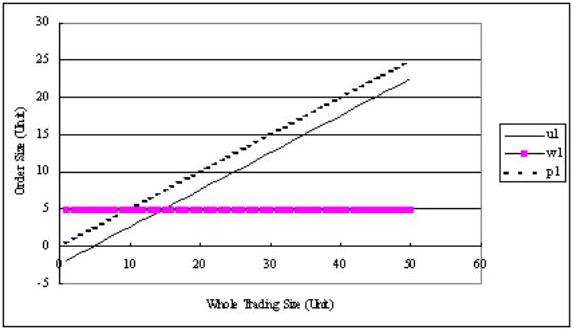
\includegraphics[width=10cm,height=6cm]{fg_l1n.png}
\end{center}
\caption[$R_1$ and $u_1^*$, $w_1^*$, and $p_1^*$ without constraints]
{{\bf $R_1$ ($x$-axis) and $u_1^*$, $w_1^*$, and $p_1^*$ ($y$-axis) without constraints.}
 \quad $u_1^*$, $w_1^*$, and $p_1^*$ are linear functions of $R_1$.}\label{fg_l1}
\end{figure}

\begin{figure}
\begin{center}
 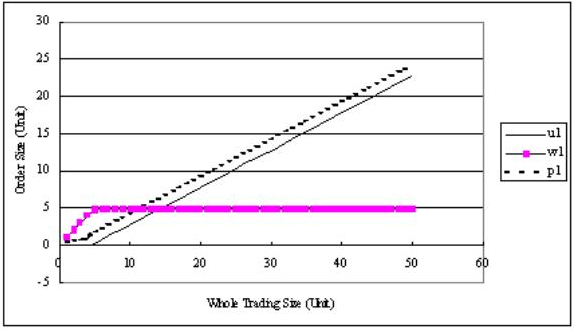
\includegraphics[width=10cm,height=6cm]{fg_l2n.png}
\end{center}
\caption[$R_1$ and $u_1^*$, $w_1^*$, and $p_1^*$ with non-negative constraint]
{{\bf $R_1$ ($x$-axis) and $u_1^*$, $w_1^*$, and $p_1^*$ ($y$-axis) with non-negative constraint.}
 \quad $u_1^*$, $w_1^*$, and $p_1^*$ are linear functions of $R_1$ for large $R_1$.}\label{fg_l2}
\end{figure}

%%%%%%%%%%%%%%%%%%%%%
\subsection{Multiple Period Case}\label{sec_l23}
The results in two period case can be extended to $T$ period case by Markov decision process since $C_1^*(R_1)$ is sum of square of $R_1$ and a constant.  Specifically, immediate application of two period case provides $T-1^{th}$ period strategy as
\[ %begin{equation}\label{eq_l19}
 \left\{
  \begin{array}{ll}
   \displaystyle p_{T-1}^* = -\frac{(ra_{T-1}-2a_T)a_{T-1}R_{T-1}}{2\{(1-r)a_{T-1}+a_T\}}, \\
   \displaystyle \frac{w_{T-1}^*}{2\sigma_{T-1}}= \frac{(1-r)a_{T-1}}{2\{(1-r)a_{T-1}+a_T\}}\frac{\phi(\frac{w_{T-1}^*}{2\sigma_{T-1}})}{\Phi(-\frac{w_{T-1}^*}{2\sigma_{T-1}})},\\
   \displaystyle u_{T-1}^*= \frac{p_{T-1}^*}{a_{T-1}}-\frac{w_{T-1}^*}{2},\\
  \end{array}
  \right.
\] %end{equation}
and the optimal cost is $\displaystyle C_{T-1}^*(R_{T-1})=\frac{\{4a_T-r^2a_{T-1}\}a_{T-1}}{4\{(1-r)a_{T-1}+a_T\}}R_{T-1}^2+constant.$  Since the optimal cost in the two period case is $a_2 R_2^2$, $i^{th}$ period strategy $(i=T-2,\cdots,1)$ is calculated similarly as
\[ %begin{equation}\label{eq_l20}
 \left\{
  \begin{array}{ll}
   \displaystyle p_i^* = -\frac{(ra_i-2A_i)a_iR_i}{2\{(1-r)a_i+A_i\}}, \\
   \displaystyle \frac{w_i^*}{2\sigma_i}= \frac{(1-r)a_i}{2\{(1-r)a_i+A_i\}}\frac{\phi(\frac{w_i^*}{2\sigma_i})}{\Phi(-\frac{w_i^*}{2\sigma_i})},\\
   \displaystyle u_i^*= \frac{p_i^*}{a_i}-\frac{w_i^*}{2}\\
  \end{array}
  \right.
\] %end{equation}
where $A_i\ (i=1,\cdots,T-1)$ is defined backward recursively as $\displaystyle
A_i=\frac{\{4A_{i+1}+r^2a_i\}a_i}{4\{(1-r)a_i+A_{i+1}\}}\ (i=T-2,\cdots,1)$ with
$\displaystyle A_{T-1}=\frac{\{4a_T+r^2a_{T-1}\}a_{T-1}}{4\{(1-r)a_{T-1}+a_T\}}$.

Figure \ref{fg_l3} shows a numerical example which illustrates changes of optimal market and limit order size over time.  In this numerical example, we assume that market order, all the realized $M_i$ turn out to be zero ($T=11, R_1=100, r=0, a_i=1, \sigma_i=10$ for $i=1,\cdots,11$).

\begin{figure}[htbp]
\begin{center}
 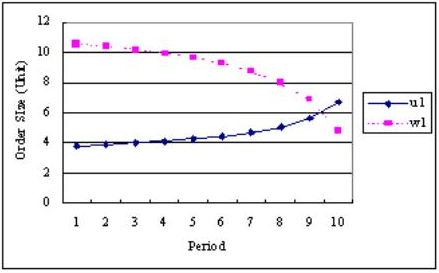
\includegraphics[width=10cm,height=6cm]{fg_l3n.png}
\end{center}
\caption[Time dependency of limit order and market order]
{{\bf Time dependency of limit order and market order} ($T=11$,
 $R_1=100$, $a_i=1$, $\sigma_i=10$ for $i=1, \cdots, 11$).
 \quad We assumed that market order, $M_i$, was revealed to be zero all the time.
 We can see that more limit orders are tried at the early stage of execution, and they are gradually replaced
with market orders.}\label{fg_l3}
\end{figure}

\begin{figure}[htbp]
\begin{center}
 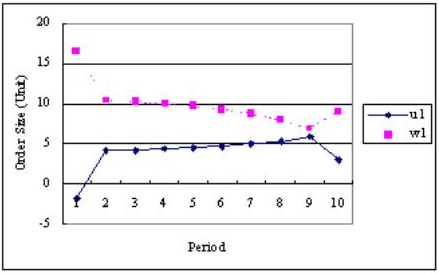
\includegraphics[width=10cm,height=6cm]{fg_l4n.png}
\end{center}
\caption[Time dependency of limit order and market order]
{{\bf Time dependency of limit order and market order} ($T=11$, $R_1=100$, $a_1=a_{11}=1.5$,
$\sigma_1=\sigma_{11}=15$, $a_i=1$, $\sigma_i=10$ for $i=2, \cdots, 10$).
 \quad We assumed that market order, $M_i$, was revealed to be zero all the time.
 Comparing to Figure \ref{fg_l3}, we can see that limit orders are avoided when $a_i$ and $\sigma_i$ are high
due to high expected cost, and market orders are preferred due to high option values.}\label{fg_l4}
\end{figure}

We can see that more limit orders are tried at the early stage of execution, and they are gradually replaced with market orders if limit orders are not executed.  Also, a case when $a_i$ and $\sigma_i$ depend on period is worth observing in order to analyze a whole day execution, since Jain and Joh (1988) find that $a_i$ and $\sigma_i$ are high at the opening and closing of a day.  Figure \ref{fg_l4} shows a numerical example in which $a_1=a_{11}=1.5$ and $\sigma_1=\sigma_{11}=15$, and all the other parameters are the same as in Figure \ref{fg_l3}.  Comparing to Figure \ref{fg_l3}, we can see that market orders are avoided when  $a_i$ and $\sigma_i$ are high due to high expected cost, and limit orders are preferred due to high option values.

Regarding statistical errors in estimating parameters, empirical studies such as Uno and Yamada (1993) and Jain and Joh (1988) report that the patterns of market impact coefficients, the price volatility, and the market trading volume are rather stable.

%%%%%%%%%%%%%
\section{Variations of Single Limit Order Model}\label{sec_l3}
In this section, we analyze several variations of the standard model in Section \ref{sec_l2}.  Although two period models are analyzed for clarity of comparison with the standard model, multiple period extension is possible in each case.

\subsection{Risk Averse Traders}
Since limit orders have uncertainty in execution, risk averse traders may prefer market orders.  When we measure risk by variance of total purchase amount, cost function can be defined as
\begin{eqnarray}\label{eq_l21}
  C_1(R_1) & = & \ex{ \sum_{j=2}^2 \delta_j \epsilon_j R_j + \sum_{i=1}^2 P_i \{(1-r) D_i +r R_i\}} \nonumber \\
      &   & +\lambda \var{ \sum_{j=2}^2 \delta_j \epsilon_j R_j + \sum_{i=1}^2 P_i \{(1-r) D_i +r R_i\}} \nonumber \\
      & = & \ex{ \sum_{i=1}^2 P_i \{(1-r) D_i +r R_i\}}+\lambda \var{\sum_{j=2}^2 \delta_j \epsilon_j R_j + \sum_{i=1}^2 P_i \{(1-r) D_i +r R_i\}}
\end{eqnarray}
where the definitions of $P_i$ and $D_i$ are the same as those in risk neutral case, $\lambda$ is a risk premium, and $V$ is the variance at the first period.

Although it is difficult to solve (\ref{eq_l21}), changes of fundamental cost tends to be much larger than the uncertainly of market impact in practice.  Therefore, we ignore uncertainty of market impact, which makes the solution a linear function as in the risk neutral case.  That is, cost function can be approximated by 
\begin{eqnarray*}\label{eq_l22}
  C_1(R_1) & \approx & \ex{\sum_{i=1}^2 P_i \{(1-r) D_i +r R_i\}}+\lambda \var{\delta_2 \epsilon_2 R_2} \nonumber \\
      & = & \ex{P_1 \{(1-r) D_1 +r R_1\}+a_2(R_1-D_1)^2}+\lambda \delta_2^2 \ex{ (R_1-D_1)^2}.
\end{eqnarray*}
Therefore, all we have to do is to replace $a_2$ of the solution in the risk neutral case with $(a_2+\lambda \delta_2^2)$.

Our optimal execution duration for risk averse traders is not very sensitive to trade size as in Almgren and Chriss (2001), which contradicts practical intuition.  This is because variance type risk measure is employed in order to implement dynamic programming.  As a result, it is recommended in practice to use both Konishi and Makimoto (2001) for execution scheduling problem and this analysis for order placing problem.

%%%%%%%%%%%%%%%%%%%%%%%%
\subsection{Visible Public Market Orders}
Up to this section, we assume that the trader knows just the expectation of the public limit orders and the distribution of the public market orders, but not concrete order sizes.  In this section however, we analyze the case when the trader monitors the public order book, and all the current period information is available.  Regarding the future periods, we continue to assume that the trader knows only the distribution and not the size of public market orders as in the previous cases.

As we have mentioned, not all traders can monitor all the public limit order books at TSE, only member security brokers are allowed to watch without time lag.  Also, even member security brokers have to choose which stocks to monitor among thousands of listed stocks.  This section estimates the value of monitoring public order books, comparing cost with that in Section \ref{sec_l2}.  

Let $b_1(p)$ and $s_1(p)$ denote volume of public buy and sell limit orders at price $p$ in the first period, respectively, and $M_i$ denote volume of excess public market order at the $i^{th}$ period.  Without loss of generality, we can assume that 
\[ %begin{equation}\label{eq_l23}
  \left\{
  \begin{array}{ll}
   b_1(p)=0, & \quad \mbox{if} \quad p>0, \\
   s_1(p)=0, & \quad \mbox{if} \quad p<0
  \end{array}
  \right.
\] %end{equation}
because buy limit order is synthesized by buy market order and sell limit order, and sell limit order is synthesized by sell market order and buy limit order.

Market orders, buy limit orders at higher price than execution price, and sell limit orders at lower price than execution price are executed, and the trader do not distinguish market and limit orders since not only market orders but also limit orders are surely executed.  Therefore, let $V_1$ denote the sum of the trader's market order and buy limit orders at higher prices than execution price.  Also, in order to complete the execution, we assume that all the remaining orders are placed as market order in the second period.  In this case, market impact $P_1$ is determined so as to balance total buy orders and sell orders.  Among them, since the trader's execution volume is $V_1$, expected purchase cost is $\ex{(P_1+Q_1)V_1}=P_1V_1$.  Also, execution volume of public buy and sell orders is $\displaystyle \int_{P_1}^{\infty} b_1(p) dp$ and $\displaystyle \int_{-\infty}^{P_1} s_1(p) dp$, respectively.  Therefore,
\[ %begin{equation}\label{eq_l24}
  V_1+M_1+\int_{P_1}^{\infty} b_1(p) dp-\int_{-\infty}^{P_1} s_1(p) dp=0.
\] %end{equation}

Regarding the second period, we assume that limit order exists at any prices for the constant amount $1/a_i$, and that the ratio of permanent market impact is $r$ as in the previous cases.  Consequently, there are sell limit orders of $1/a_i$ above price $Q_2+rP_1$ and buy limit orders of $1/a_i$ below price $Q_2+rP_1$ in the second period.  In this case, our problem can be formulated as follows:
\begin{equation}\label{eq_l25}
  \mbox{(P)} \ \ \left|
  \begin{array}{ll}
    \mbox{minimize} & \quad C_1(R_1)= P_1 \{(1-r) V_1 +r R_1\}+a_2(R_1-V_1)^2 \\
    \mbox{s.t.} & \displaystyle \quad V_1+M_1+\int_{P_1}^{\infty} b_1(p) dp-\int_{-\infty}^{P_1} s_1(p) dp=0.
  \end{array}
  \right.
\end{equation}
We can easily derive the optimal $V_1^*$ at least numerically once $Q_1$, $R_1$, $a_2$, $b_1(p)$, $s_1(p)$, and $M_1$ are given.


In the rest of this section, we analyze a linear market impact case in order to compare the results with those in Section \ref{sec_l2}:
\begin{eqnarray*}
  b_1(p) & = & \left\{
  \begin{array}{ll}
   0, & \quad \mbox{if} \quad p>0, \\
   \frac{1}{a_1}, & \quad \mbox{if} \quad p<0,
  \end{array}
  \right. \label{eq_l26}\\
  s_1(p) & = & \left\{
  \begin{array}{ll}
   \frac{1}{a_1}, & \quad \mbox{if} \quad p>0, \\
   0, & \quad \mbox{if} \quad p<0.
  \end{array}
  \right. \label{eq_l27}
\end{eqnarray*}
Since the constraint in (\ref{eq_l25}) is
\[ %begin{equation}\label{eq_l28}
  V_1+M_1=\frac{P_1}{a_1},
\] %end{equation}
our objective function is
\begin{eqnarray}\label{eq_l29}
  C_1(R_1) & = & P_1 \{(1-r) V_1 +r R_1\}+a_2(R_1-V_1)^2 \nonumber \\
      & = & \{(1-r)a_1+a_2\}V_1^2+[\{(1-r)M_1+rR_1\}a_1-2Ra_2]V_1+(rM_1a_1+2Ra_2).
\end{eqnarray}
$V_1$ which minimizes (\ref{eq_l29}) satisfies
\[ %begin{equation}\label{eq_l30}
  \pdif{C_1}{V_1}=2\{(1-r)a_1+a_2\}V_1+\{(1-r)M_1+rR_1\}a_1-2Ra_2=0.
\] %end{equation}
Therefore, the optimal order size $V_1^*$ is
\[ %begin{equation}\label{eq_l31}
  V_1^*=\frac{-\{(1-r)M_1+rR_1\}a_1+2R_1a_2}{2\{(1-r)a_1+a_2\}},
\] %end{equation}
and the optimal expected cost $C_1^*(R_1)$ is
\[ %begin{equation}\label{eq_l32}
  C_1^*(R_1) = \frac{-(1-r)^2a_1^2 M_1^2+2\{r(1-r)a_1+2a_2\}R_1 a_1 M_1+(4a_2-r^2a_1)a_1R_1^2}{4\{(1-r)a_1+a_2\}}.
\] %end{equation}
If we collect large samples in order to compare the optimal expected cost with the result in Section \ref{sec_l2}, $M_i$ follows normal distribution $N(0,\sigma_i)$.  Therefore, the average of $C_1^*(R_1)$ becomes
\[ %begin{equation}\label{eq_l33}
  \ol{C_1^*(R_1)} = \frac{(4a_2-r^2a_1)a_1R_1^2-(1-r)^2\sigma_1^2a_1^2}{4\{(1-r)a_1+a_2\}}.
\] %end{equation}
Difference between $\ol{C_1^*(R_1)}$ and the minimal cost in Section \ref{sec_l2} is
\[ %begin{equation}\label{eq_l34}
  \frac{-(1-r)^2\sigma_1^2a_1^2}{4\{(1-r)a_1+a_2\}} + \frac{\{(1-r)a_1+2a_2\}(1-r)a_1\sigma_1^2\phi^2(\frac{w_1}{2\sigma_1})}{2\{(1-r)a_1+a_2\}\Phi(\frac{w_1}{2\sigma_1})} - a_2\sigma_1^2\{2\Phi(\frac{w_1}{2\sigma_1})-1\},
\] %end{equation}
which corresponds to economical value of monitoring the public order book, which is significant when $a_1$ and $\sigma_1$ are large.  Since the trader is assumed to be risk neutral, economical value of monitoring seems independent of $R_1$.  However in practice, traders closely monitor stocks of large trades because risk averse traders try to avoid uncertainty of market impact, and because execution of larger trades takes a longer time, which makes the economical value of monitoring large.

As we have mentioned, at TSE, only member security brokers can monitor the public order book without time lag, but not general traders.  Therefore, the economical value of monitoring is a component of the membership value.  Also, even brokers have to pay some ``cost" of infrastructure and labors to monitor the public order book, and therefore, choose stocks to monitor among thousands of listed stocks.  Our formula evaluates the value of monitoring in order to justify costs of monitoring and provides criteria for selecting stocks to monitor.


%%%%%%%%%%%%%%%%%%%%%%%%%%%%%%
\section{Multiple Limit Order Model}\label{sec_l4}
Result of the standard model in Section \ref{sec_l2} can be extended to a case with $N$ limit orders.  However, since calculation is extremely complicated, it is difficult to derive explicit solution.  Therefore, in this section, we just explain some characteristics of the optimal execution strategy derived numerically.  We study two period case for simplicity.

Let $p_{ij}\ (i=1,\cdots,N, \ j=1,\cdots,T)$ and $w_{ij}\ (i=1,\cdots,N, \ j=1,\cdots,T)$ denote
$i^{th}$ base limit order prices at the $j^{th}$ period and size of corresponding limit order sizes
where $p_{ij}>p_{kj}$ for $i<k$.  Also, let $u_j$ denote market order size, and define $v_{0j} \define u_j$ and $\displaystyle v_{ij} \define v_{0j}+\sum_{k=1}^i w_{kj}.$  Then, similar calculation leads to the expected cost at the first period $C_1$ as
\begin{eqnarray}
  C_1 & = &  \{(1-r)a_1+a_2\}v_{01}^2+(ra_1-2a_2)R_1v_{01}+a_2R_1^2+Q_1R_1 \nonumber \\
      &   &  -\sum_{i=1}^N [\{(1-r)a_1+a_2\}(v_{i-1,1}+\frac{p_{i1}}{a_1})+(ra_1-2a_2)R_1] \nonumber \\
      &   & \quad \quad \{(v_{i-1,1}-\frac{p_{i1}}{a_1})\Phi(-\frac{1}{\sigma_1}(v_{i-1,1}-\frac{p_{i1}}{a_1}))-\sigma_1\phi(-\frac{1}{\sigma_1}(v_{i-1,1}-\frac{p_{i1}}{a_1}))\} \nonumber \\
      &   &  +\sum_{i=1}^N [\{(1-r)a_1+a_2\}(v_{i1}+\frac{p_{i1}}{a_1})+(ra_1-2a_2)R_1] \nonumber \\
      &   & \quad \quad \{(v_{i1}-\frac{p_{i1}}{a_1})\Phi(-\frac{1}{\sigma_1}(v_{i1}-\frac{p_{i1}}{a_1}))-\sigma_1\phi(-\frac{1}{\sigma_1}(v_{i1}-\frac{p_{i1}}{a_1}))\} \nonumber \\
      &   &  +a_2\sigma_1^2\sum_{i=1}^N \{\Phi(-\frac{1}{\sigma_1}(v_{i-1,1}-\frac{p_{i1}}{a_1}))-\Phi(-\frac{1}{\sigma_1}(v_{i1}-\frac{p_{i1}}{a_1}))\}. \label{eq_l35}
\end{eqnarray}
Also, the first order conditions of optimality is given as
\begin{eqnarray}
  \pdif{C_1}{v_{01}} & = &  2\{(1-r)a_1+a_2\}v_{01}+(ra_1-2a_2)R_1 - [2\{(1-r)a_1+a_2\}v_{01}+(ra_1-2a_2)R_1]
  \nonumber \\
  & & \times \Phi(-\frac{1}{\sigma_1}(v_{01}-\frac{p_{11}}{a_1}))
        +(1-r)a_1\sigma_1 \phi(-\frac{1}{\sigma_1}(v_{01}-\frac{p_{11}}{a_1})), \label{eq_l36} \\
  \pdif{C_1}{v_{k1}} & = & - [2\{(1-r)a_1+a_2\}v_{k1}+(ra_1-2a_2)R_1]\Phi(-\frac{1}{\sigma_1}(v_{k1}-\frac{p_{k+1,1}}{a_1})) \nonumber \\
  & & +(1-r)a_1\sigma_1 \phi(-\frac{1}{\sigma_1}(v_{k1}-\frac{p_{k+1,1}}{a_1})) + [2\{(1-r)a_1+a_2\}v_{k1}+(ra_1-2a_2)R_1] \nonumber \\
  & & \times \Phi(-\frac{1}{\sigma_1}(v_{k1}-\frac{p_{k1}}{a_1}))-(1-r)a_1\sigma_1 \phi(-\frac{1}{\sigma_1}(v_{k1}-\frac{p_{k1}}{a_1})), \label{eq_l37} \\
  \pdif{C_1}{v_{N1}} & = & [2\{(1-r)a_1+a_2\}v_{N1}+(ra_1-2a_2)R_1]\Phi(-\frac{1}{\sigma_1}(v_{N1}-\frac{p_{N1}}{a_1})) \nonumber \\
  & & -(1-r)a_1\sigma_1 \phi(-\frac{1}{\sigma_1}(v_{N1}-\frac{p_{N1}}{a_1})), \label{eq_l38} \\
  a_1\pdif{C_1}{p_{k1}} & = & + [2\{(1-r)a_1+a_2\}\frac{p_{k1}}{a_1}+(ra_1-2a_2)R_1]\Phi(-\frac{1}{\sigma_1}(v_{k-1,1}-\frac{p_{k1}}{a_1})) \nonumber \\
                     &   & +\{(1-r)a_1+2a_2\}\sigma_1 \phi(-\frac{1}{\sigma_1}(v_{k-1,1}-\frac{p_{k1}}{a_1}))
                           - [2\{(1-r)a_1+a_2\}\frac{p_{k1}}{a_1}+(ra_1-2a_2)R_1] \nonumber \\
     & & \times \Phi(-\frac{1}{\sigma_1}(v_{k1}-\frac{p_{k1}}{a_1}))-\{(1-r)a_1+2a_2\}\sigma_1 \phi(-\frac{1}{\sigma_1}(v_{k1}-\frac{p_{k1}}{a_1})). \label{eq_l39}
\end{eqnarray}

Figure \ref{fg_l5} compares the optimal costs derived numerically from (\ref{eq_l36}) to (\ref{eq_l39}) for various numbers of limit orders when $a_1=a_2=1$, $\sigma_1=10$, $r=0$, and $R_1=50$.  Although the optimal cost is a decreasing function of the number of limit orders, cost reduction decreases as the number of limit orders increases.  This result supports the effectiveness of the single limit order model.

Figure \ref{fg_l6} shows the corresponding optimal base limit order prices and their sizes.  We can see that the limit order size is symmetrical.  Although sizes increase as limit order prices depart from the center of symmetry, this is because limit orders are dense around the center.  The density of limit orders is unimodal, similar to the single limit order model.

\begin{figure}[htbp]
\begin{center}
 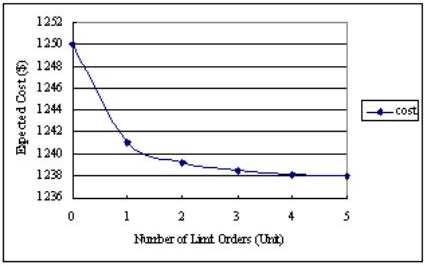
\includegraphics[width=10cm,height=6cm]{fg_l5n.png}
\end{center}
\caption[Number of limit orders and the expected cost]
{{\bf Number of limit orders ($x$-axis) and the expected cost ($y$-axis).}
 \quad This graph compares the optimal costs for various numbers of limit orders.
 Although the optimal cost is a decreasing function of the number of limit orders, cost reduction decreases as
the number of limit orders increases.
 This result supports the effect of the single limit order model.}\label{fg_l5}
\end{figure}

\begin{figure}[htbp]
\begin{center}
 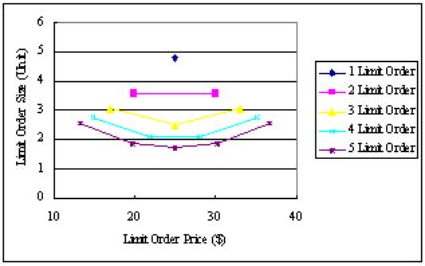
\includegraphics[width=10cm,height=6cm]{fg_l6n.png}
\end{center}
\caption[Optimal base limit order prices and their sizes]
{{\bf Optimal base limit order prices ($x$-axis) and their sizes ($y$-axis).}
 \quad We can see that the limit order size is indeed symmetrical.
 Although sizes increase as limit orders depart from the center of symmetry, this is because limit orders are
dense arround the center.
 The density of limit orders is unimodal, similar to single limit order model.}\label{fg_l6}
\end{figure}


Numerical solution suggests the following conjecture about the optimal solution although the proof of the optimality has not yet been completed. 
\begin{conjecture}\label{con_l1}
\begin{equation} \label{eq_l40}
 v_{i1}^*+v_{N-i,1}^* = \frac{p_{i+1,1}^*}{a_1} + \frac{p_{N-i,1}^*}{a_1} = -\frac{(ra_1-2a_2)R_1}{2{(1-r)a_1+a_2}}, \quad \mbox{for even } N,
\end{equation}
and
\begin{equation} \label{eq_l41}
 v_{i+1,1}^*+v_{N-i,1}^* = \frac{p_{i1}^*}{a_1} + \frac{p_{N-i,1}^*}{a_1} = -\frac{(ra_1-2a_2)R_1}{2{(1-r)a_1+a_2}}, \quad \mbox{for odd } N.
\end{equation}
\end{conjecture}

Conjecture \ref{con_l1} can be explained as follows.  First of all, because (\ref{eq_l35}) does not change even if we switch $\displaystyle v_{i1}-\frac{p_{i+1,1}}{a_1}$ and $\displaystyle -\left(v_{N-i,1}-\frac{p_{N-i,1}}{a_1}\right)$,
\[ %begin{equation} \label{eq_l101}
  v_{i1}^*-\frac{p_{i+1,1}^*}{a_1}=-\left(v_{N-i,1}^*-\frac{p_{N-i,1}^*}{a_1}\right).  
\] %end{equation}
If $N$ is even, because $\displaystyle v_{a\frac{N}{2}}^*-\frac{p_{\frac{N}{2}+1}^*}{a_1}=-(v_{a\frac{N}{2}}^*-\frac{p_{\frac{N}{2}}^*}{a_1})$ and $\displaystyle \pdif{C_1}{v_{a\frac{N}{2}}}=0$,
\[ %begin{equation} \label{eq_l102}
  v_{a\frac{N}{2}}^*=-\frac{(ra_1-2a_2)R_1}{2\{(1-r)a_1+a_2\}}.
\] %end{equation}
Also, because $\displaystyle v_{a\frac{N}{2}}^*-\frac{p_{\frac{N}{2}+1}^*}{a_1}=-(v_{a\frac{N}{2}}^*-\frac{p_{\frac{N}{2}}^*}{a_1})$,
\[ %begin{equation} \label{eq_l103}
  p_{\frac{N}{2}}^*+p_{\frac{N}{2}+1}^*=-\frac{(ra_1-2a_2)a_1R_1}{2\{(1-r)a_1+a_2\}}.
\] %end{equation}
Further, because $\displaystyle v_{a\frac{N}{2}-1}^*-\frac{p_{\frac{N}{2}}^*}{a_1}=-(v_{a\frac{N}{2}+1}^*-\frac{p_{\frac{N}{2}+1}^*}{a_1})$,
\[ %begin{equation} \label{eq_l104}
v_{a\frac{N}{2}-1}^*+v_{a\frac{N}{2}+1}^*=-\frac{(ra_1-2a_2)R_1}{2\{(1-r)a_1+a_2\}}.
\] %end{equation}
Similarly, because $\displaystyle v_{a\frac{N}{2}+i}^*-\frac{p_{\frac{N}{2}+i+1}^*}{a_1}=-(v_{a\frac{N}{2}-i}^*-\frac{p_{\frac{N}{2}-i}^*}{a_1})$,
\[ %begin{equation} \label{eq_l105}
p_{\frac{N}{2}-i}^*+p_{\frac{N}{2}+i+1}^*=-\frac{(ra_1-2a_2)a_1R_1}{2\{(1-r)a_1+a_2\}}.
\] %end{equation}
Also, since $\displaystyle v_{a\frac{N}{2}-i-1}^*-\frac{p_{\frac{N}{2}-i}^*}{a_1}=-(v_{a\frac{N}{2}+i+1}^*-\frac{p_{\frac{N}{2}+i+1}^*}{a_1})$,
\[ %begin{equation} \label{eq_l106}
v_{a\frac{N}{2}-i-1}^*+v_{a\frac{N}{2}+i+1}^*=-\frac{(ra_1-2a_2)R_1}{2\{(1-r)a_1+a_2\}.}
\] %end{equation}
Similar argument holds for the case if $N$ is odd.

By (\ref{eq_l40}) and (\ref{eq_l41}), we can reason by analogy that $p_{i1}$ and $v_{i1}$ are linear functions of $R_1$, and therefore, $w_{i1}$ are constants just as in the single limit order model.


%%%%%%%%%%%%%%%%%
\section{Closing Remarks}\label{sec_l5}
This chapter analyses the optimal selection of market and limit orders in a series of single price batch auctions when the expectation of the limit order book is given.  We derive the analytical solution of a single limit order model for risk neutral traders, and then extend the result for risk averse traders.  Regarding the execution at each period, we find that the optimal limit order size is independent of the whole trade size so as to balance the non-linearity of execution volume and price.  In contrast, the limit order price and the market order size are linear functions in order to balance trading costs across trading periods.  Regarding the execution throughout the trading session, market orders replace limit orders as time passes, and necessity of completing execution grows.  Further, if trading volume and price volatility are larger at the opening and closing of the trading session as in the practical markets, more limit orders are tried at the opening and closing.

Although most traders know the public order book as expectations as in our model, member security brokers are allowed to monitor the public order book without time lags.  So, we evaluate the value of monitoring public order books and provide criteria for selecting stocks to monitor.

Although our results can be extended to multiple limit order models mathematical analysis is left for further research.  Besides, while this chapter analyzes batch auctions for simplicity, continuous auction is also of interest.  Also, although this chapter assumes randomness comes only from the number of market orders, the number of limit orders are also stochastic in practice.  Further, we can extend our research to risk averse traders who uses VWAP as a reference price.  Besides, while this chapter performs partial equilibrium type analysis in which public orders are given exogenously, general equilibrium analysis which studies how each trader's strategy interferes is left for further research.

%%%%%%%%%%%%%%%%%%%%%
\section{Appendix}\label{sec_lappendix}

\subsection{Proof of Proposition \ref{prop_l1}}
In two period case,
\begin{eqnarray*} \label{eq_l42}
  C_1(R_1) & = & \ex{ \pi_1(\psi_1) \{(1-r) \kappa_1(\psi_1) + r R_1 \}+ a_2(R_1-\kappa_1(\psi_1,M_1)^2} \nonumber \\
      & = &  \int_{-(\u1)}^{\infty}\{a_1(m_1+u_1)\{(1-r)u_1+rR_1\}+a_2(R_1-u_1)^2\}f_1(m_1)dm_1 \nonumber \\
      &   &  +\int_{-(\v1)}^{-(\u1)}\{p_1\{(1-r)(-m_1+\frac{p_1}{a_1})+rR_1\}+a_2(R_1+m_1-\frac{p_1}{a_1})^2\}f_1(m_1)dm_1 \nonumber \\
      &   &  +\int_{-\infty}^{-(\v1)}\{a_1(m_1+v_1)\{(1-r)v_1+rR_1\}+a_2(R_1-v_1)^2\}f_1(m_1)dm_1 \nonumber \\
      & = &  \int_{-(\u1)}^{\infty}[a_1\{rR_1+(1-r)u_1\}m_1+(a_1+a_2-ra_1)u_1^2-(2a_2-ra_1)R_1u_1]f_1(m_1)dm_1 \nonumber \\
      &   &  +\int_{-(\v1)}^{-(\u1)} a_2m_1^2+\{2a_2R_1+((r-1)a_1-2a_2)\frac{p_1}{a_1}\}m_1 \nonumber \\
      &   & +\{(1-r)a_1+a_2\}(\frac{p_1}{a_1})^2+(ra_1-2a_2)R_1\frac{p_1}{a_1} ]f_1(m_1)dm_1 \nonumber \\
      &   &  +\int_{-\infty}^{-(\v1)}[a_1\{rR_1+(1-r)v_1\}m_1+(a_1+a_2-ra_1)v_1^2-(2a_2-ra_1)R_1v_1]f_1(m_1)dm_1 \nonumber \\
      &   & +a_2R_1^2.
\end{eqnarray*}
Using the following equations,
\begin{eqnarray*}
  \int_{-\infty}^{-a} x f_1(x) dx & = &  -\sigma_1^2 f_1(a),  \label{eq_l43}\\
  \int_{a}^{b} x^2 f_1(x)dx       & = &  \int_{a}^{b} \sigma_1^2 f_1(x)dx -[\sigma_1^2 x f_1(x)]_a^b,  \label{eq_l44}
\end{eqnarray*}
we obtain the following result,
\begin{eqnarray*} \label{eq_l45}
  C_1(R_1) & = &  \{(1-r)a_1+a_2\}v_{01}^2+(ra_1-2a_2)R_1v_{01}+a_2R_1^2 \nonumber \\
      &   &  - [\{(1-r)a_1+a_2\}(u_1+\frac{p_1}{a_1})+(ra_1-2a_2)R_1]\{(\u1)F_1(-(\u1))-\sigma_1^2f_1(-(\u1))\} \nonumber \\
      &   &  + [\{(1-r)a_1+a_2\}(v_1+\frac{p_1}{a_1})+(ra_1-2a_2)R_1]\{(\v1)F_1(-(\v1))-\sigma_1^2f_1(-(\v1))\} \nonumber \\
      &   &  +a_2\sigma_1^2 \{F_1(-(\u1))-F_1(-(\v1))\}
\end{eqnarray*}
where $F_1(x)= \int_{-\infty}^x f_1(y) dy.$
 The desired result now follows by noting
\[
 F_1(w) = \Phi(\frac{w}{\sigma_1}), \qquad \sigma_1^2 f_1(w) = \sigma_1 \phi(\frac{w}{\sigma_1})
\]
where $\displaystyle \phi(x)=\frac{1}{\sqrt{2\pi}}exp(-\frac{x^2}{2})$
and $\Phi(x)=\int_{-\infty}^x \phi(y) dy$.

%%%%%%%%%%%%%%
\subsection{Proof of Proposition \ref{prop_l2}}
Define $\displaystyle \overline{u}_1=\frac{\u1}{\sigma_1}$ and
$\displaystyle \overline{v}_1=\frac{\v1}{\sigma_1}$.
  Since
\begin{eqnarray}
 & & F_1(-(\u1))=\Phi(-\overline{u}_1), \label{eq_l46}\\
 & & F_1(-(\v1))=\Phi(-\overline{v}_1), \label{eq_l47}\\
 & & \displaystyle f_1(-(\u1))=\frac{1}{\sigma_1}\phi(-\overline{u}_1), \label{eq_l48}\\
 & & \displaystyle f_1(-(\v1))=\frac{1}{\sigma_1}\phi(-\overline{v}_1), \label{eq_l49}
\end{eqnarray}
$C_1(R_1)$ can be rewritten as,
\begin{eqnarray} \label{eq_l50}
  C_1(R_1) & = &  [\{(1-r)a_1+a_2\}(\frac{p_1}{a_1})^2+(ra_1-2a_2)R_1\frac{p_1}{a_1}+a_2\sigma_1^2] \nonumber \\
      &   &  +[\{(1-r)a_1+a_2\}(\sigma_1^2\overline{u}_1^2+2\sigma_1\frac{p_1}{a_1}\overline{u}_1)+(ra_1-2a_2)R_1\sigma_1\overline{u}_1-a_2\sigma_1^2]\Phi(\overline{u}_1) \nonumber \\
      &   &  +[\{(1-r)a_1+a_2\}(\sigma_1^2\overline{v}_1^2+2\sigma_1\frac{p_1}{a_1}\overline{v}_1)+(ra_1-2a_2)R_1\sigma_1\overline{v}_1-a_2\sigma_1^2]\Phi(-\overline{v}_1) \nonumber \\
      &   &  +[\{(1-r)a_1+a_2\}(\sigma_1^2\overline{u}_1+2\sigma_1\frac{p_1}{a_1})+(ra_1-2a_2)R_1\sigma_1]\phi(\overline{u}_1) \nonumber \\
      &   &  -[\{(1-r)a_1+a_2\}(\sigma_1^2\overline{v}_1+2\sigma_1\frac{p_1}{a_1})+(ra_1-2a_2)R_1\sigma_1]\phi(-\overline{v}_1) \nonumber \\
      &   &  +a_2R_1^2.
\end{eqnarray}
We then prove that the optimality and the uniqueness of the solution.  First, define 
\begin{eqnarray*}
  & & a = (1-r)a_1 + a_2, \qquad A = a_2, \qquad \sigma = \sigma_1, \\
  & & \beta = (ra_1 - 2a_2)R_1, \qquad \gamma = p_1/a_1, \qquad x = \overline{u}_1, \qquad y = \overline{v}_1,
\end{eqnarray*}
and
\[
  G(x) \define x \Phi(x) + \phi(x).
\]
Also, we represent function parameters by subscripts as $\Px = \Phi(x)$ and $\gx = G(x).$  According to (\ref{eq_l50}),
\begin{eqnarray}
  C_1(R_1)
   & = & a \gamma^2 + \beta \gamma + A \sigma^2 + [a (\sigma^2 x^2 + 2 \sigma x \gamma)
         + \beta \sigma x - A\sigma^2] \Px
         + [a (\sigma^2 y^2 + 2 \sigma y \gamma) + \beta \sigma y - A \sigma^2] \Pmy \nonumber \\
   &   & + [a (\sigma^2 x + 2\sigma \gamma) + \beta \sigma] \px
       - [a (\sigma^2 y + 2\sigma \gamma) + \beta \sigma] \py + A R_1^2  \nonumber \\
   & = & A \sigma^2 + AR_1^2 + a \gamma^2 + 2 a \sigma \left( x \Px + \px
         + y \Pmy - \py + \frac{\beta}{2a\sigma}  \right) \gamma \nonumber \\
   &   & + \sigma \left[ \left(
         a \sigma x^2 + \beta x - A \sigma \right) \Px + (a \sigma x + \beta) \px +
         \left( a \sigma y^2 + \beta y -A \sigma \right) \Pmy - (a \sigma y + \beta) \py
         \right] \nonumber \\
   & = & A\sigma^2 + AR_1^2 + a \gamma^2 + 2 a \sigma \left( \gx - \gmy
         + \frac{\beta}{2a\sigma} \right) \gamma \nonumber \\
   &   & + \sigma \left[ (a\sigma x + \beta) \gx - (a\sigma y + \beta) \gmy
         - A \sigma \{ \Px + \Pmy \} \right] \nonumber \\
   & = & A\sigma^2 + AR_1^2 + a \left[ \gamma + \sigma \left( \gx - \gmy
         + \frac{\beta}{2a\sigma} \right) \right]^2 \nonumber \\
   &   & + a \sigma^2 \left[ x \gx - y \gmy + \frac{\beta}{a\sigma} (\gx - \gmy) - \frac{A}{a} (\Px + \Pmy)
         \right] - a \sigma^2 \left( \gx - \gmy + \frac{\beta}{2a\sigma} \right)^2 \nonumber \\
   & = & A\sigma^2 + AR_1^2  - \frac{\beta^2}{4a} + a \left[ \gamma
         + \sigma \left( \gx - \gmy + \frac{\beta}{2a\sigma} \right) \right]^2 \nonumber \\
   &   & + a \sigma^2 \left[ x \gx - y \gmy - \frac{A}{a} ( \Px + \Pmy )
         - \left( \gx - \gmy \right)^2 \right]. \label{eq_l51}
\end{eqnarray}
Define the quotient of the last term of (\ref{eq_l51}) by $a \sigma^2$ as
\[ %begin{equation}\label{eq_l52}
  H(x,y) \define x \gx - y \gmy - \frac{A}{a} ( \Px + \Pmy )
        - \left( \gx - \gmy \right)^2.
\] %end{equation}
We minimize $C_1$ on $\calS = \{ (x,y)\ : \ -\infty < x <\infty, y \geq x \}$.

\begin{lemma}\label{lem_l1}
  \quad The minimum of $H$ exists on $\calS$.
\end{lemma}

\begin{proof}
Since $H(x,y)=H(-y,-x)$, $H(x,y)$ is symmetrical about $y=-x$.  Therefore, we have only to analyze on
 $\calS' = \{ (x,y)\ : -\infty < x < \infty, y \geq |x| \}.$  According to Abramowitz and Stegun (1972) p.932,
\[ %begin{equation}\label{eq_l53}
  \frac{\px}{x} \left( 1 - \frac{1}{x^2} + \frac{3}{x^4} - \frac{15}{x^6} \right) <
  \Pmx < \frac{\px}{x} \left( 1 - \frac{1}{x^2} + \frac{3}{x^4} + \frac{15}{x^6} \right), \qquad
  x > 0,
\] %end{equation}
and therefore,
\begin{eqnarray*}
  & & x + \px \left( \frac{1}{x^2} - \frac{3}{x^4} - \frac{15}{x^6} \right) < \gx
      < x + \px \left(\frac{1}{x^2} - \frac{3}{x^4} + \frac{15}{x^6} \right), \qquad x > 0, \label{eq_l54} \\
  & & \px \left( \frac{1}{x^2} - \frac{3}{x^4} - \frac{15}{x^6} \right) < \gmx
      < \px \left(\frac{1}{x^2} - \frac{3}{x^4} + \frac{15}{x^6} \right), \qquad x > 0. \label{eq_l55}
\end{eqnarray*}
Consequently, limits along the point $\calS'$ where $(sy,y)\ (-1 \leq s \leq 1)$ is given by
\[
 \lim_{y \rightarrow + \infty} H(sy,y) = \left\{
 \begin{array}{ll}
   -A/a, \quad & s > 0, \\
   -A/2a+\p0^2, & s = 0, \\
   0, & s < 0.
 \end{array}
 \right.
\]
Therefore, $H(x,y)$ is a function bounded from the bottom.  Further, since $H(0,0)=-A/a \leq \lim_{y \rightarrow +\infty} H(sy,y)$, $H(x,y)$ takes the minimum at a finite $(x,y)$.
\end{proof}

Since $\gamma$ can take any value, the minimization of $C$ by $(x, y, \gamma)$ is equivalent to the minimization of $H$ by $(x, y)$ with $\gamma = - \sigma ( \gx - \gmy + \beta/2a\sigma ).$  From the first order condition of the optimality,
\begin{eqnarray}
  \pdif{H}{x}
   & = & \gx + x \Px - \frac{A}{a} \px - 2 ( \gx - \gmy ) \Px = 0, \label{eq_l56} \\
  \pdif{H}{y}
   & = & - \gmy + y \Pmy + \frac{A}{a} \py - 2 ( \gx - \gmy ) \Pmy = 0 \label{eq_l57}
\end{eqnarray}
are necessary conditions.  By canceling $A/a$ from (\ref{eq_l56}) and (\ref{eq_l57}),
\begin{eqnarray*}
  \lefteqn{\py \left[ \gx + x \Px - 2 ( \gx - \gmy ) \Px \right]
    + \px \left[ - \gmy + y \Pmy - 2 ( \gx - \gmy ) \Pmy \right]} \nonumber \\
  & & \hspace{1.0cm} = 2 \py \Px [ x - ( \gx - \gmy )] + 2 \px \Pmy [ y - ( \gx - \gmy )] \nonumber \\
  & & \hspace{1.0cm} = 2 [ \py \Px ( \gmy - \gmx ) + \px \Pmy ( \gy - \gx ) ] \nonumber \\
  & & \hspace{1.0cm} = 0. \label{eq_l58}
\end{eqnarray*}
Define
\[ %begin{equation}\label{eq_l59}
  I(x,y) \define \px \Pmy (\gy - \gx) + \Px \py (\gmy - \gmx),
\] %end{equation}
and we have the following lemma.
\begin{lemma}\label{lem_l6}
 \quad For any $x$, $I(x,x)=I(x,-x)=0$.  Further, for any $x$ and $y > |x|$, $I(x,y)>0$.
\end{lemma}

Lemma \ref{lem_l6} shows that the first order condition of the optimality is satisfied only by $y=x$ and $y=-x$.  If we substitute $y=x$ (\ref{eq_l56}), we have
\begin{eqnarray*}
 \left. \pdif{H}{x} \right|_{y=x}
  & = & \gx + x \Px - \frac{A}{a} \px - 2 ( \gx - \gmx ) \Px \\
  & = & \gx + x \Px - \frac{A}{a} \px - 2 x\Px \\
  & = & \px - \frac{A}{a} \px \\
  & = & 0,
\end{eqnarray*}
which contradicts $0<A/a<1$.  Next, if we substitute $y=-x$, we have
\begin{equation}\label{eq_l60}
  \left. \pdif{H}{x} \right|_{y=-x} = 2 x \Phi(x) + \left( 1 - \frac{A}{a} \right) \phi(x) = 0.
\end{equation}
Regarding the solution of (\ref{eq_l60}), we have the following lemma.
\begin{lemma}\label{lem_l2}
 \quad Define $M(x) \define (ax+b)\Phi(x)+c\phi(x)$ where $a>0$ and $a>c$.  Then, $M(x)=0$ has a unique solution with positive derivative.
\end{lemma}
\begin{proof}
Direct calculation shows that
\[ %begin{equation} \label{eq_l61}
  M'(x)=a\Phi(x)+b\phi(x)+(a-c)x\phi(x),
\] %end{equation}
and
\[ %begin{equation} \label{eq_l62}
  M''(x)=\phi(x)\{-(a-c)x^2-bx+(2a-c)\}.
\] %end{equation}
Therefore, $M''(x)=0$ has two real solutions across which $M''(x)$ turns from negative to positive once, and then negative again.  Together with $\displaystyle \lim_{x \to -\infty} M'(x) =0$ and $\displaystyle \lim_{x \to \infty} M'(x) = a>0$, $M'(x)$ has a unique solution $x^*$ and,
\begin{equation} \label{eq_l63}
 \left\{
  \begin{array}{ll}
   M'(x)<0, \quad x<x^*, \\
   M'(x)>0, \quad x>x^*.
  \end{array}
  \right.
\end{equation}
Further, together with $\displaystyle \lim_{x \to -\infty} M(x) =0$ and $\displaystyle \lim_{x \to \infty} M(x) = \infty$, $M(x)=0$ has a unique solution where $M'(x)>0$.
\end{proof}

By Lemma \ref{lem_l2}, $x$ that satisfies (\ref{eq_l60}) is uniquely determined.  Consequently, $x=x^*$ is determined as the unique solution of (\ref{eq_l60}), and then, $y^* = -x^*$ and $\gamma^* = -\beta/2a$.

\bigskip

\noindent {\bf Proof of Lemma \ref{lem_l6}} \quad
It is easy to show $I(x,x)=I(x,-x)=0$.  We consider the case of $y>|x|$.  We first calculate partial derivatives of $I$ by $y$.  
\begin{eqnarray*}
  I_1(x,y)
   & \define & \frac{\partial}{\partial y} I(x,y) \\
   & = & \Px (-y \py \gmy - \py \Pmy) + \px (-\py \gy + \Pmy \Py) + \Px \gmx y \py + \px \gx \py, \\
  I_2(x,y)
   & \define & \frac{\partial}{\partial y} I_1(x,y) \\
   & = & \py [ \Px \{ (y^2-1) \gmy + 2y \Pmy + \py \} + \px (y\gy + 1 - 3\Py) -(y^2-1)\Px\gmx - \px \gx y ], \\
  J_2(x,y)
   & \define & \Px \{ (y^2-1) \gmy + 2y \Pmy + \py \} + \px (y\gy + 1 - 3\Py) -(y^2-1)\Px\gmx - \px \gx y, \\
  J_3(x,y)
   & \define & \frac{\partial}{\partial y} J_2(x,y) \\
   & = & \Px \{ 2y \gmy - (y^2-3) \Pmy -3y\py \} + \px ( \gy +y \Py -3\py ) -2 \Px \gmx y - \px \gx, \\
  J_4(x,y)
   & \define & \frac{\partial}{\partial y} J_3(x,y) \\
   & = & 2 [ \Px \{ \gmy - 2y \Pmy + (2y^2-3) \py \} + \px (\Py + 2y \py) - \Px \gmx ], \\
  J_5(x,y)
   & \define & \frac{\partial}{\partial y} J_4(x,y) \\
   & = & 2 [ \Px \{ -3 \Pmy -(2y^3-9y) \py \} - \px (2y^2-3) \py ], \\
  J_6(x,y)
   & \define & \frac{\partial}{\partial y} J_5(x,y) \\
   & = & 2 \py \{ (2y^4-15y^2+12) \Px + (2y^3-7y) \px \}.
\end{eqnarray*}
Since 
\[
 I(x,y) \approx \px \Pmy \gy - \Px \gmx \py \approx \Pmx \gx \py
\]
for $y \rightarrow +\infty$, we obtain\footnote{For a function $f$, we define $f(\pm \infty)=\lim_{t \rightarrow \pm \infty} f(t)$.  Also, $a+0\ (a-0)$ represents conversion to $a$ from the above (from the below)}
\[
 I(x,+\infty) = 0+0.
\]
Together with $I(x,x) = I(x,-x) = 0$, if we prove the existence and the uniqueness of $y>|x|$ where $I_1(x,y)=0$ for any $x$, we can prove that $I(x,y)>0$ for $y>|x|$.

In order to see the sign change of $J_6$, we first analyze
\[
 K(y) \define \frac{2y^4-15y^2+12}{2y^3-7y} = y - \frac{8y^2-12}{2y^3-7y}.
\]
Then,
\begin{eqnarray*}
  \dif{K}{y}
    & = & 1 + \frac{16y^4 - 16y^2 +84}{(2y^3-7y)^2} \\
    & = & 1 + \frac{4 (2y^2 - 1)^2 +80}{(2y^3-7y)^2} \\
    & > & 0, \qquad\qquad (\forall x \neq 0, \pm \sqrt{7/2}).
\end{eqnarray*}
Therefore, $K(y)$ is monotone increasing for $y \neq 0, \pm \sqrt{7/2}$, and shifts according to the following table.
\[
\begin{array}{|c||c|c|c|c|c|c|c|c|c|c|c|c|c|c|} \hline
  y & -\infty & \cdots & \multicolumn{2}{c|}{{\displaystyle -\frac{\sqrt{15+\sqrt{129}}}{2}}} & \cdots
    & \multicolumn{2}{c|}{{\displaystyle -\sqrt{\frac{7}{2}}}} & \cdots
    & \multicolumn{2}{c|}{{\displaystyle -\frac{\sqrt{15-\sqrt{129}}}{2}}} & \cdots & \multicolumn{2}{c|}{0} \\ \hline
  2y^4-15y^2+12 & +\infty & + & \multicolumn{2}{c|}{0} & - & \multicolumn{2}{c|}{-} & - & \multicolumn{2}{c|}{0} & +
    & \multicolumn{2}{c|}{+} \\ \hline
  2y^3-7y & -\infty & - & \multicolumn{2}{c|}{-} & - & \multicolumn{2}{c|}{0} & + & \multicolumn{2}{c|}{+} & +
    & \multicolumn{2}{c|}{0} \\ \hline
  K(y) & -\infty & \nearrow & \multicolumn{2}{c|}{0} & \nearrow & +\infty & -\infty & \nearrow & \multicolumn{2}{c|}{0}
    & \nearrow & +\infty & -\infty \\ \hline
\end{array}
\]
\[
\begin{array}{|c||c|c|c|c|c|c|c|c|c|c|c|c|c|c} \hline
  y & \multicolumn{2}{c|}{0} & \cdots & \multicolumn{2}{c|}{{\displaystyle \frac{\sqrt{15-\sqrt{129}}}{2}}} & \cdots
    & \multicolumn{2}{c|}{{\displaystyle \sqrt{\frac{7}{2}}}} & \cdots
    & \multicolumn{2}{c|}{{\displaystyle \frac{\sqrt{15+\sqrt{129}}}{2}}} & \cdots & +\infty \\ \hline
  2y^4-15y^2+12 & \multicolumn{2}{c|}{+} & + & \multicolumn{2}{c|}{0} & - & \multicolumn{2}{c|}{-} & -
    & \multicolumn{2}{c|}{0} & + & +\infty \\ \hline
  2y^3-7y & \multicolumn{2}{c|}{0} & - & \multicolumn{2}{c|}{-} & - & \multicolumn{2}{c|}{0} & +
    & \multicolumn{2}{c|}{+} & + & +\infty \\ \hline
  K(y) & +\infty & -\infty & \nearrow & \multicolumn{2}{c|}{0} & \nearrow & +\infty & -\infty & \nearrow
    & \multicolumn{2}{c|}{0} & \nearrow & +\infty \\ \hline
\end{array}
\]
Since $J_6(x,y)=2 \py \Px (2y^3-7y) [K(y) + \px/\Px]$, $J_6(x,y)$ turns from ``positive, negative, positive, negative, and positive" for $y=-\infty \rightarrow +\infty$.  Henceforth, we represent this shifts as\footnote{Although we are interested only the area of $y>|x|$, we analyze the change of the sign for $y=-\infty \riinf$}

\begin{equation}\label{eq_l64}
 \sgn(J_6) = (+-+-+).
\end{equation}
Next, we analyze the sign change of $J_5$.
\begin{eqnarray}
  J_5(x,-\infty) & = & - 6 \Px \ \ < 0, \label{eq_l65} \\
  J_5(x,+\infty) & = & \lim_{y \rightarrow +\infty} -4 \Px y^3 \py = 0-0. \label{eq_l66}
\end{eqnarray}
By (\ref{eq_l64}), (\ref{eq_l65}), and (\ref{eq_l66}), three cases are possible for the sign change of $J_5$, $\sgn(J_5)=(-),\ (-+-),\ (-+-+-)$.  We next show that $\sgn(J_5)=(-+-+-)$ is not viable.  When $x$ is given, we define the smallest $y$ as $y_*$ among four $y$ that satisfy $J_6(x,y)=0$.  Then, $y_*<-\sqrt{15+\sqrt{129}}/2$.\footnote{Although $y_*$ depends on $x$, we do not write $x$ explicitly for the simplicity of the representation.  Besides, $y_*<-\sqrt{15+\sqrt{129}}/2$ holds for any $x$.}
Since $J_6(x,y_*)=0,$
\begin{eqnarray*}  
  J_5(x,y_*)
   & = & - 2 \Px (2y_*^2-3) \phi_{y_*} \left\{ \frac{3 \Phi_{-y_*} + (2y_*^3-9y_*)\phi_{y_*}}{(2y_*^2-3)\phi_{y_*}}
         + \frac{\px}{\Px} \right\} \\
   & = & - 2 \Px (2y_*^2-3) \phi_{y_*} \left\{ \frac{3\Phi_{-y_*} + (2y_*^3-9y_*)\phi_{y_*}}{(2y_*^2-3)\phi_{y_*}}
         - \frac{2y_*^4-15y_*^2+12}{2y_*^3-7y_*} \right\}.
\end{eqnarray*}

\begin{lemma}\label{lem_l3}
 \quad For any $x$, $J_5(x,y^*)<0.$
\end{lemma}

\begin{proof}
Since $2y_*^2-3>0$, it is sufficient to show $L(y^*)>0$ where
\[
  L(y) \define \frac{3\Phi_{-y} + (2y^3-9y)\phi_{y}}{(2y^2-3)\phi_{y}} - \frac{2y^4-15y^2+12}{2y^3-7y}.
\]
Since $y_* < -\sqrt{15+\sqrt{129}}/2<-2$, it is sufficient to show $L(y)>0$ for $y<-2$.
\[
 L(y) = \frac{1}{2y^2-3} \left( \frac{3\Pmy}{\py} + \frac{4y^4-6y^2+36}{2y^3-7y} \right)
      = \frac{1}{2y^2-3} \left( \frac{3\Pmy}{\py} + 2y + \frac{4}{y} + \frac{8}{2y^3-7y} \right).
\]
Since both $4/y$ and $8/(2y^3-7y)$ are decreasing for $y<-2$,
\[
 \frac{4}{y} + \frac{8}{2y^3-7y} > \frac{4}{-2} + \frac{8}{2 \cdot (-2)^3-7 \cdot (-2)} = -4.
\]
Consequently,
\[
 L(y) > \frac{1}{2y^2-3} \left( \frac{3 \Phi_{2}}{\sqrt{2\pi}} e^{y^2/2} + 2y -4 \right)
      > \frac{1}{2y^2-3} \left( 1.137 e^{y^2/2} + 2y -4 \right), \qquad y < -2.
\]
When we define
\[
 M(y) \define 1.136 e^{y^2/2} + 2y -4,
\]
we obtain
\[
 M(-2) > 0, \qquad\quad
 \dif{M}{y} = 1.136 y e^{y^2/2} + 2 < 0, \qquad \forall y<-2.
\]
Therefore, we have shown $M(y)>0$ for $y<-2$, i.e., $L(y)>0$.
\end{proof}

Since Lemma \ref{lem_l3} shows that the first relative minimum of $J_5$ is negative, $\sgn(J_5)=(-+-+-)$ never happens, and therefore, only $\sgn(J_5)=(-),\ (-+-)$ are possible cases.

Next, regarding the sign change of $J_4$,
\begin{eqnarray*}
 J_4(x,-\infty) & = & \lim_{y \rightarrow -\infty} - 6 \Px y = + \infty, \label{eq_l67} \\
 J_4(x,+\infty) & = & 2 \Pmx \gx \ \ > 0. \label{eq_l68}
\end{eqnarray*}
Together with $\sgn(J_5)=(-),\ (-+-)$, there are two possible cases, $\sgn(J_4)=(+),\ (+-+)$.

Next, regarding the sign change of $J_3$,
\begin{eqnarray*}
 J_3(x,-\infty) & = & \lim_{y \rightarrow -\infty} - 3 \Px y^2 = - \infty, \label{eq_l69} \\
 J_3(x,+\infty) & = & \lim_{y \rightarrow +\infty} 2 \Pmx \gx y = + \infty. \label{eq_l70}
\end{eqnarray*}
Together with $\sgn(J_4)=(+),\ (+-+)$, there are two possible cases, $\sgn(J_3)=(-+),\ (-+-+)$.

Next, regarding the sing change of $J_2$,
\begin{eqnarray*}
 J_2(x,-\infty) & = & \lim_{y \rightarrow -\infty} - \Px y^3 = + \infty, \label{eq_l71} \\
 J_2(x,+\infty) & = & \lim_{y \rightarrow +\infty} \Pmx \gx y^2 = + \infty. \label{eq_l72}
\end{eqnarray*}
Together with $\sgn(J_3)=(-+),\ (-+-+)$, there are two possible cases,
\begin{equation}\label{eq_l73}
 \sgn(J_2)=(+), \quad (+-+), \quad (+-+-+).
\end{equation}

Finally, regarding the sign change of $I_1$,
\begin{eqnarray}
 I_1(x,-\infty) & = & \lim_{y \rightarrow -\infty} \Px y^2 \py = 0 + 0, \label{eq_l74} \\
 I_1(x,x) & = & 0, \label{eq_l75} \\
 I_1(x,+\infty) & = & \lim_{y \rightarrow +\infty} - \Pmx \gx y \py = 0 - 0. \label{eq_l76}
\end{eqnarray}

\bigskip

\noindent (I) When $x \geq 0$
The following lemma holds for
\[
  J_2(x,x)=2 x \Px \Pmx + \px - 2\px \Px.
\]
\begin{lemma}\label{lem_l4}
\begin{equation}\label{eq_l77}
 J_2(x,x) \quad \left\{
 \begin{array}{ll}
 > 0, \quad & x>0, \\
 = 0, \quad & x=0, \\
 < 0, \quad & x<0.
 \end{array}
 \right.
\end{equation}
\end{lemma}
\begin{proof}
When we define
\[
 A(x) \define J_2(x,x) = 2x \Px \Pmx + \px - 2 \px \Px,
\]
\begin{eqnarray*}
 A_1(x) & \define & \dif{}{x}A(x) = 2 \Px \Pmx + 2x \px \Pmx - x \px - 2 \px^2, \\
 A_2(x) & \define & \dif{}{x}A_1(x) = \px ( 4 \Pmx - 2 \Px - 2 x^2 \Pmx+ 2 x \px -1 + x^2), \\
 B(x) & \define &  4 \Pmx - 2 \Px - 2 x^2 \Pmx+ 2 x \px -1 + x^2, \\
 B_1(x) & \define & \dif{}{x}B(x)= -2 \left( 2 \px + 2 x \Pmx - x \right)
             =      -4x \left( \frac{\px}{x} + \Pmx - \frac{1}{2} \right), \\
 C(x) & \define & \frac{\px}{x} + \Pmx - \frac{1}{2}, \\
 C_1(x) & \define & \dif{}{x}C(x) = - \px \left( 2 + \frac{1}{x^2} \right).
\end{eqnarray*}
Since $C_1(x)<0$ for any $x \neq 0$, and
\begin{eqnarray*}
  C(-\infty) & = & 1/2, \\
  C(0-0) & = & -\infty, \\
  C(0+0) & = & +\infty, \\
  C(+\infty) & = & -1/2,
\end{eqnarray*}
and toghether with $B_1(x) = -4x C(x),$
\begin{equation}\label{eq_l78}
 \sgn(B_1) = (+-+), \qquad x = -\infty \rightarrow +\infty.
\end{equation}
With (\ref{eq_l78}) and
\begin{eqnarray*}
  B(-\infty) & = & - \infty, \\
  B(0) & = & 0, \\
  B(+\infty) & = & + \infty, \\
  B_1(0) & = & -4 \p0 < 0,
\end{eqnarray*}
we obtain
\begin{equation}\label{eq_l79}
  \sgn(B) = \sgn(A_2) = (-+-+), \qquad x = -\infty \rightarrow +\infty.
\end{equation}
With (\ref{eq_l79}) and
\begin{eqnarray*}
  A_1(-\infty) & = & 0-0, \\
  A_1(0) & = & \frac{1}{2} - \frac{1}{\pi} > 0, \\
  A_1(+\infty) & = & 0-0,
\end{eqnarray*}
we obtain
\begin{equation}\label{eq_l80}
  \sgn(A_1) = (-+-).
\end{equation}
With (\ref{eq_l80}) and
\begin{eqnarray*}
  A(-\infty) & = & 0-0, \\
  A(0) & = & 0, \\
  A(+\infty) & = & 0+0,
\end{eqnarray*}
we finally obtain
\[ %begin{equation}\label{eq_l81}
  A(x) \ \ \left\{
  \begin{array}{ll}
   > 0, \quad & x>0, \\
   = 0, & x=0, \\
   < 0, & x<0.
  \end{array}
  \right.
\] %end{equation}
\end{proof}

By Lemma \ref{lem_l4}, when $x>0$, $I_1(x,y)$ crosses the $x$-axis from the negative to positive at $y=x$.  Also, when $I_1(x,y)$ moves from positive to positive at $y=x$.  In both cases, $I_1(x,y)=0$ has the unique solution on $y>|x|=x$ by equations from (\ref{eq_l73}) to (\ref{eq_l76}).\footnote{By this argument, $\sgn(J_2)=(+),\ (+-+)$ never happens actually.}

\bigskip

\noindent (II) When $x<0$
The following lemma holds for
\[
 I_1(x,-x) = \px \{ x^2 \Px + x \px + \Px (\Pmx - \Px) \}.
\]

\begin{lemma}\label{lem_l5}
 \quad For any $x \neq 0$, $I_1(x,-x)>0.$
\end{lemma}
\begin{proof}
\begin{eqnarray*}
  A(x) & \define & \frac{I_1(x,-x)}{\px} = x \gx + \Px - 2 \Px^2, \\ 
  A_1(x) & \define & \dif{}{x}A(x) = 2 (\gx - 2\px \Px), \\
  A_2(x) & \define & \dif{}{x}A_1(x) = 2(\Px + 2x \px \Px - 2\px^2), \\
  A_3(x) & \define & \dif{}{x}A_2(x) = 2\px (1+2\Px-2x^2 \Px + 6x \px), \\
  B(x) & \define & 1+2\Px-2x^2 \Px + 6x \px, \\
  B_1(x) & \define & \dif{}{x}B(x) = 4 ( 2 \px - x\Px - 2 x^2 \px ), \\
  B_2(x) & \define & \dif{}{x}B_1(x) = 4 [(2x^3 - 7x) \px - \Px], \\
  B_3(x) & \define & \dif{}{x}B_2(x) = - 4 \px (2x^4-13x^2+8)
\end{eqnarray*}
\noindent 1) Regarding $B_3$

Since $\sgn(2x^4-13x^2+8)=(+-+-+)$, we obtain $\sgn(B_3)=(-+-+-)$.  Also, $B_3(x)=0$ when
\[
 x = \pm \frac{\sqrt{13 \pm \sqrt{105}}}{2}.
\]

\smallskip

\noindent 2) Regarding $B_2$

Two relative maximums are
\begin{eqnarray*}
 B_2 \left( -\frac{\sqrt{13-\sqrt{105}}}{2} \right) & \approx & 1.1159, \\
 B_2 \left( \frac{\sqrt{13+\sqrt{105}}}{2} \right) & \approx & -0.7488.
\end{eqnarray*}
Also, since $B_2(-\infty) = 0-0$, and $B_2 (+\infty) = -4+0$, we obtain $\sgn(B_2)=(-+-).$

\smallskip

\noindent 3) Regarding $B_1$

Since $B_1(-\infty) = 0-0$, $B_1(0) = 8 \p0$, and $B_1(+\infty) = - \infty$, we obtain $\sgn(B_1)=(-+-)$.

\smallskip

\noindent 4) Regarding $B$

Since $B(-\infty) = 1-0$, $B(0) = 2$, and $B(+\infty) = -\infty$, we obtain either $\sgn(B)=\sgn(A_3)=(+-)$, or $(+-+-)$.

\smallskip

\noindent 5) Regarding $A_2$

Since $A_2(-\infty) = 0+0$, and $A_2(+\infty) = 2+0$, we obtain either $\sgn(A_2)=(+)$, or $(+-+)$.

\smallskip

\noindent 6) Regarding $A_1$

Since $A_1(-\infty) = 0+0$, $A_1(0) = 0$, $A_1(+\infty) = +\infty$, and $A_2(0) > 0$, we obtain $\sgn(A_1)=(+-+).$ \footnote{Therefore, $\sgn(A_2)=(+)$ never happens.}

\smallskip

\noindent 7) Regarding $A$

Since $A(-\infty) = 0+0$, $A(0) = 0$, $A(+\infty) = +\infty$, and $A_1(0) = 0$, we obtain $\sgn(A)=(+)$.
\end{proof}

By Lemma \ref{lem_l5} and (\ref{eq_l75}), there exists an area where
$I_1(x,y)$ increases on $y \in (x, -x)$.  By equations from
(\ref{eq_l73}) to (\ref{eq_l76}), $I_1(x,y)=0$ has a unique solution
over $y>|x|=-x$.\footnote{By this argument, $\sgn(J_2)=(+),\ (+-+)$
never happens actually. }


% 02/01 changed according to ref No.2
% 02/04 inserted Fig_s4
% 02/05 changed from .emf to n.png
% 02/06 changed according to ref No.2 (by Makimoto)

%%%%%%%%%%%%%%%
%   VWAP    %%
%%%%%%%%%%%%%%%

%\setcounter{section}{0}

\chapter{Optimal Slice of a VWAP Trade}\label{chap_s}


\begin{quote}
{\bf Abstract} \quad This chapter derives a static optimal execution strategy of a VWAP trade, in which the optimal execution strategy can be calculated by an iteration of a single variable optimization, rather than by a multivariable optimization.  Analytical solutions are derived in some cases.  We show that optimal execution times lag behind expected market trading volume distribution since price volatility tends to have a positive correlation with market trading volume.  In a basket trade, execution error can be reduced by spreading out execution times according to the correlation of price movement.  We confirm our theoretical results with actual trading data and simulations.
\vspace*{0.5cm}

\end{quote}


%%%%%%%%%%%%%%%%%
\section{Introduction}\label{sec_s1}
VWAP stands for volume-weighted average price during a certain trading period, and a VWAP trade refers a trade that uses VWAP as a benchmark.  This chapter analyzes optimal execution of a VWAP trade since little academic work can be found on this issue although VWAP has become an industry standard, and several studies have been made on optimal strategies for general trade execution.

VWAP trades are overtaking fixed-price trades in stock markets these days for several reasons.  First, foreign investors and individual investors reduce trading costs by VWAP trades.  For example, foreign investors are often forced to place large orders before the market opens due to the time lag.  In a fixed-price trade, brokers, who are generally risk averse, charge a large risk premium because of the size of the risk.  However, investors can save on the risk premium by using VWAP as a benchmark because market directional risk remains the investors' responsibility. 

Second, a block trade and determination of the option strike price require high price transparency, which can be achieved with a VWAP benchmark.  In a block and option trade, brokers try to cover their exposure to price movement risk as closely to a benchmark as possible in order to avoid possible losses.  If investors use a price at a fixed time in the future as a benchmark, the closing price for instance, brokers are forced to trade intensively towards closing, which results in a huge market impact, and burdens investors with considerable costs.  However, a VWAP benchmark can reduce the market impact of hedging trades and prevent manipulation of market prices.  

Third, VWAP orders can be used to evaluate traders' performance since the effect of market directional movement, which is considered to be noise in performance measurements, is excluded in comparisons with VWAP.  As a result, a number of institutional investors such as pension funds and mutual funds place VWAP orders. 

While investors can place fixed-price orders at any time they like, VWAP orders are gathered by brokers before a trading period starts.  Brokers then match buy and sell orders, and only the surplus is executed in the market.  Note that aggregated VWAP orders tend to involve various stocks and consist of a few large orders and numerous small orders due to the characteristics mentioned above.  Further, small orders for which buyers or sellers take the trouble to use a VWAP benchmark generally have low liquidity.

In executing market trades, a VWAP trader wishes to get the average execution price as close to the market VWAP as possible to avoid price movement risk.  To do so, a VWAP trader slices a whole trade into small executions and tries to spread the executions in a well-balanced manner over the trading period, which makes VWAP trades rather labor intensive.  Therefore, it often makes sense to build a standard strategy beforehand, and execute trades automatically according to it.  A standard strategy is especially good for small orders and orders with small weights in a basket trade whose economic impact is small.  Consequently, this chapter focuses on the optimal strategy for automatic execution of small VWAP orders with low liquidity.  

As the investment business becomes increasingly competitive and understanding of the market microstructure improves, trading costs attract greater attention from both practitioners and academic researchers.  As a consequence, several studies have examined optimal trade execution strategy.  For example, Harris and Hasbrouck (1996) and Parlour (1998) analyze the choice of market and limit orders, and Bertsimas and Lo (1998) and Chapter \ref{chap_b} of this study derive an optimal slicing strategy for block trades.  Although this chapter has similar objectives to those of preceding studies, both market price and trading volume are stochastic in a VWAP trade, while only the price process is stochastic in a block trade.

Numerous studies have been done on the relationship between price volatility and market trading volume since Clark's (1973) seminal paper, including Epps and Epps (1976), Tauchen and Pitts (1983).  Karpoff (1987) summarizes these results, and Andersen (1996) proposes a modified model.  These studies, in general, support the existence of a positive correlation between price volatility and market trading volume and the autocorrelation of themselves because surprising news boosts both price volatility and market trading volume.  Besides, Jain and Joh (1988), Admati and Pfleiderer (1988), Foster and Viswanathan (1990), and Chan et al.~(1995) study intraday data and find a ``U-shaped effect," i.e., within a single day, price volatility and market trading volume tend to be higher at the opening and closing than in the middle of a trading session.  Naturally, our VWAP model reflects these findings.

Dynamic optimization, in which the actual trading strategy might be changed as new information arrives, is certainly a potential VWAP execution strategy.  However, static optimization without strategy changes works well enough, especially for small VWAP orders with low liquidity.  This is because observed variables such as the price volatility and market trading volume of stocks with low liquidity may contain statistical errors too large to be used in forecasting, and therefore, dynamic optimization is considered to be inaccurate.  For example, when market trading volume suddenly surges, it is difficult to predict whether high market trading volume is temporary or permanent even judging qualitatively.  In spite of inaccuracy and trouble related to dynamic optimization, the impact of small orders on cost efficiency is insignificant.  Consequently, static optimization is considered a reasonable alternative. 

Further, a static optimal execution strategy can be used as a benchmark for a dynamic execution strategy.  A strategy change can be evaluated by comparing the realized cost to that of a static optimal execution strategy.

For these reasons, this chapter focuses on the static optimal execution strategy of a VWAP trade.  Specifically, optimal trade decisions are made before the trading period, based on traders' expectations regarding price volatility, market trading volume, and the correlation between these values at different time of the day.  No revision is allowed in the middle of the day after the true market trading volume is observed.  

The rest of this chapter is organized as follows.  Section \ref{sec_s2} formulizes the optimal strategy.  Section \ref{sec_s3} derives solutions for single-stock cases, analyzes characteristics of the optimal strategy, and tests them against historical data.  Section \ref{sec_s4} analyzes a multiple-stock case.  Finally, Section \ref{sec_s5} concludes the analysis.

%%%%%%%%%%%%%%%%%%%%%%%
\section{Formulization of the Optimal Slicing}\label{sec_s2}
Imagine a case in which a trader buys a certain number of shares and
tries to get the average purchase price as close as possible to the
market VWAP during the trading period from time 0 to time $T$.    Let
$(\Omega, \calF, Q)$ be a probability space with a filtration
$\{ \calF_t \}$, which satisfies usual conditions.  Let $V(t)$
denote the accumulated market trading volume at time $t$ excluding the
trader's, and $v(t)$ the trader's accumulated trading volume.
 Here, $\{ V(t) \}$ is an $\{ \calF_t \}$-adapted process in $L^2$ space, and $v(t)$ is a controllable variable.  At time 0, the trader knows $v(0)=V(0)=0$ and the whole trade size $v(T)$ which is given exogenously, but not $V(t)$ for $t>0$.  We do not allow sell orders, and therefore, $v(t)$ is a non-negative increasing function as well as $V(t)$.  Further, minimum trading unit is given exogenously and normalized to one for simplicity, which makes $V(t)$ and $v(t)$ step functions, and we assume left continuous. 

Let $\{ P(s) \}$ denote a non-negative $\{ \calF_t \}$-adapted stock price process in $L^2$ space.  A trader's own VWAP is expressed as
\[
  vwap=\frac{\int_0^T P(s) dv(s)}{v(T)}.
\]

Also, the market VWAP is 
\[
  VWAP=\frac{\int_0^T P(s)d\{V(s)+v(s)\}}{V(T)+v(T)}=\frac{\int_0^T P(s)dV(s)+v(T) \times vwap}{V(T)+v(T)}.
\]
As we have mentioned, a VWAP trader tries to get his VWAP as close to the market VWAP as possible.  Generally speaking, the market impact of a VWAP trade is insignificant because the whole trade is divided into small executions.  Therefore, this chapter ignores the market impact effect and minimizes the expected squared error of the VWAP execution due to price movement.  Mathematically, our objective is represented as
\[
  \min_{v(t)} \ex{(VWAP-vwap)^2}.
\]
The following proposition holds regarding the expected squared error of the VWAP execution.

\begin{proposition}\label{prop_s1}
 \quad The expected squared error of the VWAP execution is calculated as 
\[
  W \ex{\left\{\int_0^T (X(t)-x(t))dP(t)\right\}^2}+\cov{\left(\frac{V(T)}{V(T)+v(T)}\right)^2}{\left\{\int_0^T (X(t)-x(t))dP(t)\right\}^2}
\]
where 
\[
 X(t)=\frac{V(T)-V(t)}{V(T)}, \quad x(t)=\frac{v(T)-v(t)}{v(T)},
 \quad W=\ex{\left(\frac{V(T)}{V(T)+v(T)}\right)^2}.
\]
\end{proposition}

\begin{proof}
  See Section \ref{sec_sappendix}.
\end{proof}

In this proposition, $X(t)$ and $x(t)$ stand for the ratio of remaining trading volume of the market and of the trader, respectively, and both of them are left continuous decreasing step functions.  We call $x(t)$ an execution strategy function henceforth.

Further, when $V(T)$ is sufficiently large compared to $v(T)$, $\frac{V(T)}{V(T)+v(T)}$ has a value close to one, which makes its variation small and the covariance term negligible.  Thus, we make the following assumption.

\begin{assumption}\label{ass_s1}
\quad The expected squared error can be approximated as
\begin{equation}\label{eq_s1}
  W \ex{\left\{\int_0^T (X(t)-x(t))dP(t)\right\}^2}.
\end{equation}
\end{assumption}

Since this formula is still too complicated to generate implications, further assumptions are made which are considered reasonable based on standard theories and empirical analyses.  First, the stock price process is assumed to follow a Brownian motion, similar to standard option pricing theory.  The drift term is considered to be zero because the time frame is short.  Second, according to the ``Mixture of Distribution Hypothesis" by Clark (1973) and empirical analysis by Jain and Joh (1988), there exists a relationship between price volatility and market trading volume which can be written as follows.

\begin{assumption}\label{ass_s2}
 \quad The stock price process is represented as
\[
  dP(t)=\sigma(t,V(t))dB(t),
\]
in which $\sigma(t,V(t))$ is a positive $\{ \calF_t \}$-adapted process in $L^2$ space, and $B(t)$ is a standard Brownian motion on $(\Omega, \calF, Q)$.  
\end{assumption}

 We can assume that the probability of a negative $P(t)$ is negligible because the time frame is short.

Under these assumptions, (\ref{eq_s1}) becomes
\begin{equation}\label{eq_s2}
  W \int_0^T \ex{\sigma(t,V)^2(X(t)-x(t))^2} dt.
\end{equation}
This equation gives great insight into the difficulty of certain VWAP trades: a trade with a small expected squared error is a trade large enough to make $W$ small and $w(t)$ smooth, with a stable market trading volume distribution over time, and with low price volatility.

Since our objective is to minimize the value of (\ref{eq_s2}), our problem can be further modified as,
\begin{eqnarray}
    \lefteqn{\mbox{min} \int_0^T \ex{\sigma(t,V)^2(X(t)-x(t))^2} dt} \nonumber \\
    & = & \int_0^T \ex{\sigma(t,V)^2X(t)^2}dt+ \min\int_0^T \{-2\ex{\sigma(t,V)^2X(t)}x(t)+ \ex{\sigma(t,V)^2}x(t)^2]\}dt \nonumber \\
    & = & \int_0^T \left\{ \ex{\sigma(t,V)^2X(t)^2}-\frac{\ex{\sigma(t,V)^2X(t)}^2}{\ex{\sigma(t,V)^2}} \right\} dt \nonumber \\
    &   & + \min \int_0^T \left\{ \frac{\ex{\sigma(t,V)^2X(t)}}{\ex{\sigma(t,V)^2}}-x(t)\right\}^2\ex{\sigma(t,V)^2} dt \label{eq_s3}
\end{eqnarray}
in which $x(t)$ is a controllable variable and others are given parameters.

In practice, expectations of $\sigma(t,V)^2$ and $X(t)$ vary gradually across time except at scheduled events such as batch auctions and news announcements.  Therefore, $\displaystyle \frac{\ex{\sigma(t,V)^2X(t)}}{\ex{\sigma(t,V)^2}}$ in (\ref{eq_s3}) can be assumed to be continuous almost everywhere with finite jumps.  Also, we can assume that $\displaystyle \frac{\ex{\sigma(t,V)^2X(t)}}{\ex{\sigma(t,V)^2}}$ is left continuous without loss of generality, in the same way as $X(t)$ and $x(t)$.

Let $t_k \quad (k=1,\cdots,v(T))$ denote $v(T)$ of execution times, and define $t_0=0$ and $t_{v(T)+1}=T$.  Then, $x(t)$ is a step function with $v(T)+1$ values as follows.
\begin{equation}\label{eq_s4}
  x(t)=1-\frac{k}{v(T)} \quad \mbox{if} \quad t_k < t \leq t_{k+1} \quad (k=0,\cdots,v(T)).
\end{equation}
Therefore, determination of the optimal execution strategy function $x^*(t)$ is equivalent to determination of optimal execution times $\{t_k^*\}$.  Further, a careful examination of (\ref{eq_s3}) reveals that this problem is considered to be an issue of how to approximate a function, continuous almost everywhere, with a step function as in Figure \ref{fg_s1}.

\begin{figure}[htbp]
\begin{center}
 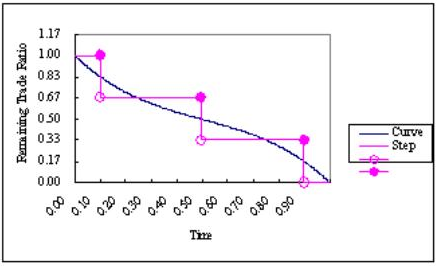
\includegraphics[width=10cm,height=5cm]{fg_s1n.png}
\end{center}
\caption[Image of $\displaystyle \frac{\ex{\sigma(t,V)^2X(t)}}{\ex{\sigma(t,V)^2}}$ and $x(t)$]
{{\bf Image of $\displaystyle \frac{\ex{\sigma(t,V)^2X(t)}}{\ex{\sigma(t,V)^2}}$ and $x(t)$} (Curve:
$\displaystyle \frac{\ex{\sigma(t,V)^2X(t)}}{\ex{\sigma(t,V)^2}}$, Step: $x(t)$).
 \quad Our problem is considered to be an issue of how to approximate
$\displaystyle \frac{\ex{\sigma(t,V)^2X(t)}}{\ex{\sigma(t,V)^2}}$, a function differentiable almost everywhere with
finite jumps, with $x(t)$, a left continuous step function with $v(T)+1$ values.}\label{fg_s1}
\end{figure}

It is possible that $t_k^*$ is equal to $t_{k+1}^*$ where $\displaystyle \frac{\ex{\sigma(t,V)^2X(t)}}{\ex{\sigma(t,V)^2}}$ jumps at batch auctions.  In this case, multiple units are executed simultaneously.  This does not detract from our argument since we ignore trading costs, including the market impact.  Note that if $v(T)$ is large enough, $x^*(t)$ can be approximated by
\[
\displaystyle x^*(t) \approx \frac{\ex{\sigma(t,V)^2X(t)}}{\ex{\sigma(t,V)^2}}.
\]

Mathematically, the following proposition holds.

\begin{proposition}\label{prop_s2}
\begin{eqnarray}
    &   & \min\int_0^T \{-2\ex{\sigma(t,V)^2X(t)}x(t)+ \ex{\sigma(t,V)^2}x(t)^2]\}dt\nonumber \\
    & = & \min \sum_{k=1}^{v(T)} \int_0^{t_k} \left[ \left\{ -\frac{2\ex{\sigma(t,V)^2X(t)}}{v(T)\ex{\sigma(t,V)^2}}+\frac{2(v(T)-k)+1}{v(T)^2}\right\}\ex{\sigma(t,V)^2}\right]dt. \label{eq_s5}
\end{eqnarray}
\end{proposition}

\begin{proof}
  See Section \ref{sec_sappendix}.
\end{proof}

Note that we can optimize each $t_k$ separately since it appears only as the upper bound of the integral on the right hand side of (\ref{eq_s5}).  The specific solution is derived in the following section.

%%%%%%%%%%%%%%%%
\section{Derivation of the Optimal Strategy: Single-Stock Case}\label{sec_s3}
In this section, we derive solutions both when price volatility is uncorrelated and correlated with market trading volume, and compare these results.

\subsection{Uncorrelated Case: $\sigma$ is uncorrelated with $V$}
In this case, the optimal execution strategy can be solved explicitly as the following proposition.

\begin{proposition}\label{prop_s3}
 \quad Under Assumptions \ref{ass_s1} and \ref{ass_s2}, and if price volatility is uncorrelated with market trading volume, optimal execution times $\{t_k^*\}$ are determined to satisfy 
\[
  \ex{X(t_k^*)} \geq \frac{2(v(T)-k)+1}{2v(T)} \geq \lim_{t \downarrow t_k^*} \ex{X(t)}.
\]
Further, the optimal execution strategy function $x^*(t)$ is solved as
\[
  x^*(t)=\frac{\lfloor (2v(T)\ex{X(t)}+1)/2 \rfloor}{v(T)},
\]
where $\lfloor x \rfloor$ represents the integer part of $x$.
\end{proposition}

\begin{proof}
  See Section \ref{sec_sappendix}.
\end{proof}

Therefore, $\{t_k^*\}$ is determined only by $\ex{X(t)}$, and is independent of expectations regarding the magnitude and term structure of price volatility.  Note that $x^*(t)$ is solved directly without solving $\{t_k^*\}$.

In practice, it used to be common to divide trading periods into equal time intervals and to allocate executions proportional to $\ex{X(t)}$.  However, this strategy (Old Strategy henceforth) comes with attendant problems, namely that as intervals are shortened in an attempt to track market trading volume more closely, more orders are placed at the opening and closing when instantaneous market trading volume is larger than in the middle of the trading session.  In contrast, our optimal strategy (New Strategy henceforth) is derived by dividing $\ex{X(t)}$ into the number of shares and executing at the middle of $\ex{X(t)}$ in each interval.  In other words, the New Strategy takes price movement risk into account and minimizes time differences in order execution.  Note that the interval with high market trading volume is not necessarily the optimal execution time.  Consequently, the New Strategy provides not only an optimal slice with the least expected squared error but also an unbiased slice for any orders even if the time intervals are infinitesimally small.

Next, we confirm our theoretical results empirically, using actual intraday data from the Tokyo Stock Exchange provided by Nikkei Quick Information Co. Ltd.  All empirical analyses in this chapter are based on trading data from October 2000 to March 2001 on the 10 stocks with the largest market capitalization.  Data from December 29, 2000 and January 4, 2001 are excluded since there was no afternoon session on these days.  We chose these large stocks in order to retain statistical accuracy since their ticks are frequent and stable.  We believe that results can be applied to other stocks since the relationship between price volatility and market trading volume is ubiquitous for all stocks as Chan et al. (1995) point out.  

Figure \ref{fg_s2} shows the standard deviation of VWAP execution errors using the Old Strategy and the New Strategy when the whole day is divided into nine intervals of 30 minutes each.  Specifically, we first estimate $\ex{X(t)}$ of each stock as the average of past trading data.  Then, in the Old Strategy, fixed number of executions are allocated proportional to the increment of $\ex{X(t)}$ for the nine intervals with the smallest rounding errors.  In the New Strategy, executions are allocated by the prescribed method.  For comparison, we assume that trades are executed at VWAP of each interval in both Old and New Strategy.  This allocation is fixed during the whole sample period, and VWAP execution errors are calculated everyday.  Finally, standard deviation of VWAP execution errors is calculated over sample stocks and dates.

According to Figure \ref{fg_s2}, the superiority of the New Strategy, especially for small orders, is evident.  The superiority is more conspicuous when time intervals are shortened, although we do not show the result here.

\begin{figure}[htbp]
\begin{center}
 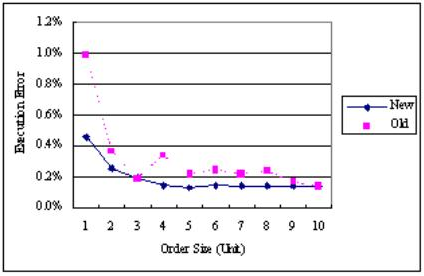
\includegraphics[width=10cm,height=6cm]{fg_s2n.png}
\end{center}
\caption[Comparison of execution strategies]
{{\bf Comparison of execution strategies.}
 \quad This graph shows the standard deviation of VWAP execution errors using the {\it old strategy} and the {\it new strategy}
($y$-axis) for different order sizes ($x$-axis) when the whole day is divided into nine intervals of 30 minutes
each.
 The superiority of the new strategy, especially for small orders, is evident.}\label{fg_s2}
\end{figure}


\subsection{ Correlated Case: $\sigma$ is a function of $V$}
In this case, the integrand in (\ref{eq_s5}) is not necessarily increasing. However, what we have to do is essentially the same; to find the upper bounds of the integrals one by one so as to minimize the area between the straight line and the curved line in Figure \ref{fg_s3}: negative if the curved line is below the straight line, positive if the curved line is above the straight line.  As we can see in Figure \ref{fg_s3}, the upper bounds fall on one of the countable points where the curved line rises to intersect the straight line (A or G for $t_k^*$, and B or H for $t_{k+1}^*$ in Figure \ref{fg_s3}).  Therefore, we have only to evaluate the integral at these points and choose one that minimizes the integral.

\begin{figure}[htbp]
\begin{center}
 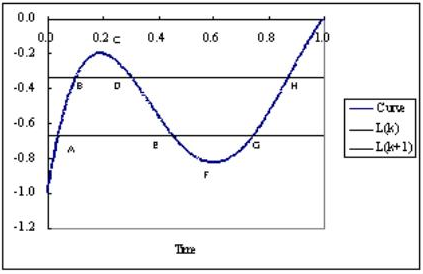
\includegraphics[width=10cm,height=6cm]{fg_s3n.png}
\end{center}
\caption[Optimization image]
{{\bf Optimization image} (curve: $\displaystyle \frac{\ex{\sigma(t,V)^2X(t)}}{\ex{\sigma(t,V)^2}}$, $L(k)$:
$\displaystyle -\frac{v(T)-k+1/2}{v(T)}$, $L(k+1)$: $\displaystyle -\frac{v(T)-(k+1)+1/2}{v(T)}$).
 \quad Although the integrand is not necessarily increasing, we still want to find the upper bounds of integrals one
 by one so as to minimize the area between the straight line and the curved line.
 It turns out that such a point falls on one of the countable points where the curved line rises to intersect
the straight line (A or G for $t_k^*$, and B or H for $t_{k+1}^*$).
 Therefore, we have only to evaluate the integral at these points and choose one that minimizes the
integral.}\label{fg_s3}
\end{figure}


Note that $t_k^*$ and $t_{k+1}^*$ chosen separately in the above procedure always satisfy $t_k^* \leq t_{k+1}^*$.  This is obvious when $t_k^*$ falls on A.  If $t_k^*$ falls on G, $\mbox{Area(ACE)} < \mbox{Area(EFG)}$ holds.  Together with $\mbox{Area(BCD)} < \mbox{Area(ACE)}$ and $\mbox{Area(EFG)} < \mbox{Area(DFH)}$, $\mbox{Area(BCD)} < \mbox{Area(DFH)}$.  Consequently, $t_{k+1}^*$ falls on H and is larger than $t_k^*$.

As a matter of fact, $\displaystyle \frac{\ex{\sigma(t,V)^2X(t)}}{\ex{\sigma(t,V)^2}}$ is usually stable and monotone decreasing in practice, as we confirm with actual data later.  Therefore, we make the following assumption in the rest of Section \ref{sec_s3}.

\begin{assumption}\label{ass_s3}
 \quad $\displaystyle \frac{\ex{\sigma(t,V)^2X(t)}}{\ex{\sigma(t,V)^2}}$ is monotone decreasing.
\end{assumption}

Under this assumption, the term in the bracket in (\ref{eq_s5})
\[
  \left\{-\frac{2\ex{\sigma(t,V)^2X(t)}}{v(T)\ex{\sigma(t,V)^2}}+\frac{2(v(T)-k)+1}{v(T)^2}\right\}
\]
is increasing and turns from negative to positive just once.  Further, even if the integrand itself  
\[
  \left\{-\frac{2\ex{\sigma(t,V)^2X(t)}}{v(T)\ex{\sigma(t,V)^2}}+\frac{2(v(T)-k)+1}{v(T)^2}\right\}\ex{\sigma(t,V)^2}
\]
is not increasing, the integrand turns from negative to positive only once since $E[\sigma(t,V)^2]$ is positive.  Consequently, we can obtain the optimal solution explicitly at such a unique point just as in the Uncorrelated Case, and the following proposition holds.  

\begin{proposition}\label{prop_s4}
 \quad Under Assumptions \ref{ass_s1} -- \ref{ass_s3}, and if price volatility is correlated with market trading volume, optimal execution times $\{t_k^*\}$ are determined to satisfy 
\[
  \ex{\sigma(t_k^*,V)^2X(t_k^*)} \geq \frac{2(v(T)-k)+1}{2v(T)}\ex{\sigma(t_k^*,V)^2} \geq \lim_{t \downarrow t_k^*} \ex{\sigma(t,V)^2X(t)}.
\]
Further, the optimal execution strategy function $x^*(t)$ is solved as
\[
  x(t)=\frac{\lfloor (\frac{2v(T)\ex{\sigma(t,V)^2 X(t)}}{\ex{\sigma(t,V)^2}}+1)/2 \rfloor}{v(T)}
\]
where $\lfloor x \rfloor$ represents the integer part of $x$.

\end{proposition}

According to Clark (1973), Jain and Joh (1988), and others, $\sigma(t,V)$ is considered to be an increasing function of market trading volume, or equivalently, an increment of $V(t)$ because surprising news boosts both $\sigma(t,V)$ and the increment of $V(t)$.  Also, since the increment of $V(t)$ tends to have a positive autocorrelation, $X(t)$ is an increasing function of the increment of $V(t)$.  Therefore, in general, the correlation between $\sigma(t,V)^2$ and $X(t)$ is positive, or equivalently, $\ex{\sigma(t,V)^2X(t)}>\ex{\sigma(t,V)^2}\ex{X(t)}$.  Consequently, $x^*(t)$ in the Correlated Case tends to become larger than in the Uncorrelated Case, which delays trade execution.  This is because once price volatility and market trading volume surge, traders have to make considerable trades to track market trading volume while execution times do not matter when these parameters remain small throughout the day.

There might be two approaches to check the monotonicity of $\displaystyle \frac{\ex{\sigma(t,V)^2X(t)}}{\ex{\sigma(t,V)^2}}$: theoretical and empirical.  In the theoretical approach, we can find sufficient conditions with existing models such as Clark (1973), Admati and Pfleiderer (1988), Andersen (1996), and others, and check that actual data satisfies such conditions.  While these conditions may take various forms, depending on parameter specifications in the models, their implications are similar: stable correlation, reasonable volatility, etc.  On the other hand, we can show the same results in the empirical approach without assuming any specific models.  Since the empirical approach is more robust, we check with past data that actual $\displaystyle \frac{\ex{\sigma(t,V)^2X(t)}}{\ex{\sigma(t,V)^2}}$ is indeed decreasing.

Table \ref{table_s1} shows the optimal allocation ratio of the VWAP execution for individual stocks in the Correlated Case, using the previous 10-stock trading data.  Prices are normalized so that those at the end of March are one.  Also, $v(t)$ is assumed to be large enough that $\displaystyle x^*(t) \approx \frac{\ex{\sigma(t,V)^2X(t)}}{\ex{\sigma(t,V)^2}}$.  $x^*(t)$ here is calculated from the average of $\sigma(t,V)^2X(t)$, and $\sigma(t,V)^2$ over the sample period.  Specifically, let $P_{d,t}$ and $V_{d,t}$ denote price and accumulated market trading volume in $d^{th}$ day $t^{th}$ interval ($d=1,\cdots,D$, $t=1,\cdots,T$).  Price change can be represented as 
\[
  \Delta P_{d,t} = \left\{
  \begin{array}{ll}
   P_{d,t}-P_{d,j-1}, \quad \mbox{for} \quad t=2,\cdots,T, \\
   P_{d,1}-P_{d-1,T}, \quad \mbox{for} \quad t=1
  \end{array}
  \right.
\]
and realized ratio of remaining trading volume as $\displaystyle X_{d,t}=\frac{V_{d,T}-V_{d,t-1}}{V_{d,T}}$.  We estimate $\ex{\sigma(t,V)^2X(t)}$ as $\displaystyle \frac{1}{D} \sum_{d=1}^D \Delta P_{d,t}^2X_{d,t}$, and estimate $\ex{\sigma(t,V)^2}$ as $\displaystyle \frac{1}{D} \sum_{d=1}^D \Delta P_{d,t}^2$.  Let $x_t^*$ denote the optimal ratio of remaining execution in the $t^{th}$ interval, then the optimal allocation ratio of the VWAP execution is given as $-(x_{t+1}^*-x_t^*)$.

\begin{table}[htbp]
\begin{center}
\begin{tabular}{|l|ccccccccc|} \hline
 Period & 1 & 2 & 3 & 4 & 5 & 6 & 7 & 8 & 9 \\ \hline
 Takeda & 0.22 & 0.09 & 0.07 & 0.10 & 0.14 & 0.04 & 0.09 & 0.07 & 0.17 \\
 Matsushita & 0.22 & 0.09 & 0.07 & 0.10 & 0.14 & 0.04 & 0.09 & 0.07 & 0.17 \\
 Sony & 0.21 & 0.09 & 0.10 & 0.09 & 0.11 & 0.07 & 0.06 & 0.10 & 0.16 \\
 Toyota & 0.23 & 0.04 & 0.12 & 0.05 & 0.13 & 0.09 & 0.06 & 0.01 & 0.27 \\
 Honda & 0.21 & 0.10 & 0.09 & 0.09 & 0.12 & 0.03 & 0.09 & 0.09 & 0.18 \\
 Mizuho & 0.19 & 0.08 & 0.08 & 0.09 & 0.11 & 0.10 & 0.08 & 0.08 & 0.18 \\
 Tokyo-Mitsubishi & 0.21 & 0.06 & 0.09 & 0.06 & 0.13 & 0.02 & 0.14 & 0.08 & 0.20 \\
 Nomura & 0.22 & 0.09 & 0.08 & 0.08 & 0.13 & 0.07 & 0.09 & 0.09 & 0.15 \\
 NTT & 0.21 & 0.08 & 0.09 & 0.07 & 0.12 & 0.06 & 0.10 & 0.07 & 0.21 \\
 NTT Docomo & 0.19 & 0.11 & 0.11 & 0.08 & 0.10 & 0.09 & 0.05 & 0.09 & 0.18 \\ \hline
\end{tabular}
\end{center}
\caption[Optimal allocation ratio of execution]{{\bf Optimal allocation ratio of execution.} \quad This table shows the optimal allocation ratio of the VWAP execution for individual stocks in the correlated case, using the previous 10 stock trading data.
  $v(t)$ is assumed to be large enough that ${\displaystyle x^*(t) \approx
\frac{\ex{\sigma(t,V)^2 X(t)}}{\ex{\sigma(t,V)^2}}}$.
 $X^*(t)$ here is calculated from the average of $\sigma(t,V)^2 X(t)$ and $\sigma(t,V)^2$ over the sampling period.
 As we expected, all the optimal allocation ratios of execution in the correlated case are positive, which means
${\displaystyle \frac{\ex{\sigma(t,V)^2 X(t)}}{\ex{\sigma(t,V)^2}}}$ is indeed monotone decreasing.}\label{table_s1}
\end{table}

As expected, all of the optimal execution allocation ratios of execution in Table \ref{table_s1} are positive, which means $\displaystyle \frac{\ex{\sigma(t,V)^2X(t)}}{\ex{\sigma(t,V)^2}}$ is indeed monotone decreasing.

Also, Figure \ref{fg_s4} shows the average of $x^*(t)$, which coincides with $\ex{X(t)}$ in the Uncorrelated Case and $\displaystyle \frac{\ex{\sigma(t,V)^2X(t)}}{\ex{\sigma(t,V)^2}}$ in the Correlated Case.  $\ex{X(t)}$ here is also estimated as an average over the sample period.  

We can see that $x^*(t)$ in the Correlated Case is, in fact, larger than in the Uncorrelated Case, which delays trade execution.  Besides, according to the same data, standard deviations of VWAP execution error are 0.127\% in the Uncorrelated Case and 0.119\% in the Correlated Case, which shows that a VWAP trade can be executed more accurately by taking into account the correlation between price volatility and market trading volume.

Main sources of these errors are considered to be statistical errors in estimating parameters and stochastic changes of parameters.  Regarding the statistical errors, empirical studies such as Uno and Yamada (1993) and Jain and Joh (1988) report that the parameters of the market impact coefficents, the price volatility, and the market trading volume are rather stable.  Regarding stochastic changes, execution errors can be reduced by dynamic optimization in Chapter \ref{chap_d}.  In practice, we further suffer price changes within the interval and discritization errors due to the minimum trading unit, both of which are considered to be proportional to the price volatility.

\begin{figure}[htbp]
\begin{center}
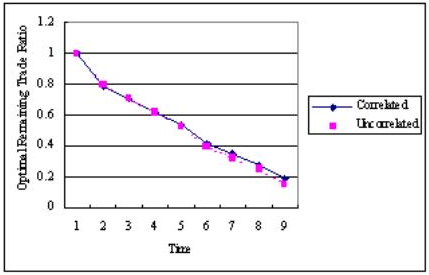
\includegraphics[width=10cm,height=6cm]{fg_s4n.png}
\end{center}
\caption[Comparison of average optimal execution strategy functions]
{{\bf Comparison of average optimal execution strategy functions.}
 \quad This graph shows the average of $x^*(t)$, which coincides with $\ex{X(t)}$ in the uncorrelated case and
$\displaystyle \frac{\ex{\sigma(t,V)^2X(t)}}{\ex{\sigma(t,V)^2}}$ in the correlated case.
 We can see that $x^*(t)$ in the correlated case is, in fact, larger than in the uncorrelated case, which delays trade
execution.}\label{fg_s4}
\end{figure}

%%%%%%%%%%%%%%%%%%%%%%%
\section{Derivation of the Optimal Strategy: Multiple-Stock Case}\label{sec_s4}
\subsection{Formulization of the Optimal Slicing}
Imagine a case with $N$ stocks.  Price, price volatility, the accumulated trading volume of the market and the trader, etc.\ of $i^{th}$ stock are represented by subscripts: $P_i(t)$, $\sigma_i(t)$, $V_i(t)$, $v_i(t)$, respectively, and satisfy similar conditions as in single-stock case.  Also, let $t_{ik} \quad (i=1,\cdots,N, k=1,\cdots,v_i(T))$ denote $v_i(T)$ of execution times of $i^{th}$ stock.   Further, define the weights of $i^{th}$ stock in the whole trade as
\[
   w_i=\frac{v_i(T)}{\sum_{j=1}^N v_j(T)}.
\]
The VWAP of the whole trade can be defined as the weighted average of the individual VWAP.  In this case, the following equation holds as Proposition \ref{prop_s1} in the single-stock case,
\begin{eqnarray*}
  \lefteqn{\ex{\{\sum_{i=1}^N w_i(VWAP_i-vwap_i)\}^2}} \\
  & = & \sum_{i=1}^N \sum_{j=1}^N W_{ij} \ex{\int_0^T (X_i(t)-x_i(t))dP_i(t)\int_0^T (X_j(t)-x_j(t))dP_j(t)} \\
  &   & + \cov{w_i\left(\frac{V_i(T)}{V_i(T)+v_i(T)}\right)w_j\left(\frac{V_j(T)}{V_j(T)+v_j(T)}\right)}{\int_0^T (X_i(t)-x_i(t)dP_i(t)\int_0^T (X_j(t)-x_j(t))dP_j(t)}
\end{eqnarray*}
where
\[
  X_i(t)=\frac{V_i(T)-V_i(t)}{V_i(T)}, \quad x_i(t)=\frac{v_i(T)-v_i(t)}{v_i(T)}, \quad W_{ij}=\ex{w_i\left(\frac{V_i(T)}{V_i(T)+v_i(T)}\right)w_j\left(\frac{V_j(T)}{V_j(T)+v_j(T)}\right)}.
\]
 
As in the single-stock case, when $V_i(T)$ is large enough compared to $v_i(T)$, $\displaystyle \frac{V_i(T)}{V_i(T)+v_i(T)}$ has a value close to one, which makes its variation small.  Therefore, the covariance term becomes negligible, and the expected squared error of the whole VWAP execution can be approximated as
\[
  \displaystyle \sum_{i=1}^N \sum_{j=1}^N W_{ij} \ex{\int_0^T (X_i(t)-x_i(t))dP_i(t)\int_0^T (X_j(t)-x_j(t))dP_j(t)}.
\]

Let stock prices follow a Brownian motion with a correlation  $\rho_{ij}(t,V_i(t),V_j(t))$, i.e.,
\[
\begin{array}{ll}
  dP_i(t)=\sigma_i(t,V_i(t))dB_i(t),\\
  dB_i(t)dB_j(t)=\rho_{ij}(t,V_i(t),V_j(t))dt,
\end{array}
\]
in which $\{ \rho_{ij}(t,V_i(t),V_j(t)) \}$ is an $\{ \calF_t \}$-adapted process in $L^2$ space,
and $\{ B_i(t) \}$ is a standard Brownian motion on $(\Omega, \calF, Q)$.
In this case, equation above becomes
\begin{equation}\label{eq_s8}
  \sum_{i=1}^N \sum_{j=1}^N W_{ij} \int_0^T \ex{\rho_{ij}(t,V_i(t),V_j(t))\sigma_i(t,V_i(t))\sigma_j(t,V_j(t))(X_i(t)-x_i(t))(X_j(t)-x_j(t))}dt
\end{equation}
and the following proposition holds for our optimization problem.

\begin{proposition}\label{prop_s5}
\begin{eqnarray*}
 \lefteqn{\min \sum_{i=1}^N \sum_{j=1}^N W_{ij} \int_0^T \ex{\rho_{ij}\sigma_i\sigma_j(X_i-x_i)(X_j-x_j)}dt} \nonumber \\
    & = & \min \sum_{i=1}^N \sum_{j=1}^N W_{ij} \sum_{k=1}^{v_i(T)+v_j(T)} \int_0^{t_k^{ij}}\left\{-\frac{\ex{\rho_{ij}\sigma_i\sigma_jX_j}}{v_i\ex{\rho_{ij}\sigma_i\sigma_j}}+\frac{x_i(t_{k-1}^{ij})x_j(t_{k-1}^{ij})-x_i(t_k^{ij})x_j(t_k^{ij})}{2}\right\} \ex{\rho_{ij}\sigma_i\sigma_j} dt \nonumber \\
    &   & +\sum_{i=1}^N \sum_{j=1}^N W_{ij}\int_0^T \ex{\rho_{ij}\sigma_i\sigma_jX_iX_j}dt \label{eq_s9}
\end{eqnarray*}
in which $\{t_k^{ij}\}$ is a sequence which renumbers $\{\{t_{ik}\},\{t_{jk'}\}\}$, and arguments in $\rho_{ij}(t,V_i(t),V_j(t))$, $\sigma_i(t,V_i(t))$, and $X_i(t)$ are omitted due to the simplicity of the representation.
\end{proposition}

\begin{proof}
  See Section \ref{sec_sappendix}.
\end{proof}

It is again a problem to determine the upper bounds of the integrals one by one, as in the single-stock case.  Therefore, once orders among $\{t_k^{ij}\}$ are assumed, we can find the solution by evaluating the integrals at countable points where the integrand turns from negative to positive, and choosing one that minimizes the integral.  However, if the order of execution times contradicts this assumption, we have to adjust them so as to minimize the corresponding integrals simultaneously.  In this case, other countable points where the sum of these integrands turns from negative to positive are also candidates. 

To determine the optimal order among $\{t_k^{ij}\}$, we need to calculate optimal solutions in several cases.  The order with the minimum expected squared error of execution is then the global optimal strategy.  In practice, we can divide the whole trade into small clusters that are hardly correlated with each other, and then find the order among highly correlated assets within each cluster.  Another effective way is to start with a stock with a large weight and then choose other parameters recursively.

Because this equation is too general to produce deep implications, we analyze a specific numerical example in the following subsection.


%%%%%%%
\subsection{Numerical Example}
% ($N=2$, $v_1(T)=v_2(T)=1$, while $\sigma_1$, $\sigma_2$, and $\rho_{12}$ are constants.)}
If $t_{11} \leq t_{12}$, (\ref{eq_s8}) becomes
\begin{eqnarray}
    &   & \int_0^{t_{11}}W_1^2\sigma_1^2(1-2\ex{X_1(s)})+2W_{12}\rho_{12}\sigma_1\sigma_2(1-\ex{X_2(s)})ds \nonumber \\
    &   & +\int_0^{t_{21}}W_2^2\sigma_2^2(1-2\ex{X_2(s)})+2W_{12}\rho_{12}\sigma_1\sigma_2(-\ex{X_1(s)})ds \label{eq_s10}
\end{eqnarray}
where $W_1=\sqrt{W_{11}}$, and $W_2=\sqrt{W_{22}}$.  Since $\sigma_1$, $\sigma_2$, and $\rho_{12}$ are constants, the integrands in (\ref{eq_s10}) become monotone increasing functions, and the optimal strategy can be solved explicitly as in Section \ref{sec_s3}.  Specifically, $t_{11}^*$ and $t_{12}^*$ are chosen so that 
\begin{equation}\label{eq_s11}
\left\{
  \begin{array}{ll}
    W_1^2\sigma_1^2(1-2\ex{X_1(t_{11}^*)})+2W_{12}\rho_{12}\sigma_1\sigma_2\{1-\ex{X_2(t_{11}^*)})=0, \\
    W_2^2\sigma_2^2(1-2\ex{X_2(t_{21}^*)})+2W_{12}\rho_{12}\sigma_1\sigma_2\{-\ex{X_1(t_{21}^*)})=0.
  \end{array}
\right.
\end{equation}
For example, if market trading volume is constant, 
\[
  \ex{X_1(t)}= \ex{X_2(t)}=1-\frac{1}{T}.
\]
Further, if $W_{12}=W_1W_2$ holds, (\ref{eq_s11}) then becomes,

\[
\left\{
  \begin{array}{ll}
    \displaystyle W_1^2\sigma_1^2(1-2\ex{X_1(t_{11}^*)})+2\rho_{12}W_1\sigma_1W_2\sigma_2\{1-\ex{X_2(t_{11}^*)}\} \\
    \displaystyle =2W_1\sigma_1(W_1\sigma_1+\rho_{12}W_2\sigma_2)\frac{t_{11}^*}{T}-W_1^2\sigma_1^2 =0,\\
    \displaystyle W_2^2\sigma_2^2(1-2\ex{X_2(t_{21}^*)})+2\rho_{12}W_1\sigma_1W_2\sigma_2\{-\ex{X_1(t_{21}^*)}\} \\
    =\displaystyle 2W_2\sigma_2(W_2\sigma_2+\rho_{12}W_1\sigma_1)\frac{t_{21}^*}{T}-W_2^2\sigma_2^2 -2\rho_{12}W_1\sigma_1W_2\sigma_2=0.
  \end{array}
\right.
\]
So,
\begin{equation}\label{eq_s13}
\left\{
  \begin{array}{ll}
    \displaystyle t_{11}^*=\frac{W_1\sigma_1T}{2(W_1\sigma_1+\rho_{12}W_2\sigma_2)}, \\
    \displaystyle t_{21}^*=\frac{(W_2\sigma_2+2\rho_{12}W_1\sigma_1)T}{2(W_2\sigma_2+\rho_{12}W_1\sigma_1)}.
  \end{array}
\right.
\end{equation}
Besides, in this case, (\ref{eq_s10}) is 
\[
  \rho_{12}W_1^4\sigma_1^4+(1+4\rho_{12}^2)W_1^3\sigma_1^3W_2\sigma_2+4\rho_{12}(1+\rho_{12}^2)W_1^2\sigma_1^2W_2^2\sigma_2^2+(1+4\rho_{12}^2)W_1\sigma_1W_2^3\sigma_2^3+\rho_{12}W_2^4\sigma_2^4.
\]
Therefore, the solution for $t_{21}^* \leq t_{11}^*$ has the same execution error due to symmetry, and so, (\ref{eq_s13}) is the optimal strategy.

Figure \ref{fg_s5} shows $t_{11}^*$ and $t_{21}^*$ for different price correlations when $W_1\sigma_1=0.2$, $W_2\sigma_2=0.1$ , and $T=1$.  If $\rho_{12}=0$, optimal execution times coincide with the solution optimized independently ($t_{11}^*=t_{21}^*=0.5$).  If $\rho_{12}>0$, optimal execution times are spread over the trading period according to correlation.  In this case, the adjustment will be larger for the stock with the smaller $W\sigma$.

\begin{figure}[htbp]
\bigskip
\begin{center}
 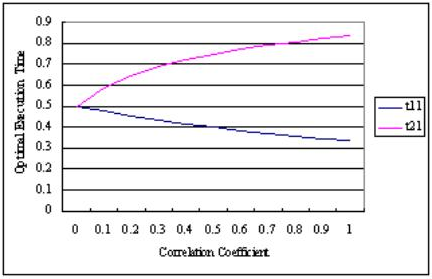
\includegraphics[width=10cm,height=6cm]{fg_s5n.png}
\end{center}
\caption[Optimal execution times for two stocks]{{\bf Optimal execution times for two stocks.}
 \quad This graph shows $t_{11}^*$ and $t_{21}^*$ for different price correlations when $W_1\sigma_1=0.2$,
 $W_2\sigma_2=0.1$,
and $T=1$.
 If $\rho_{12}=0$, optimal execution times coincide with the solution optimized independently
 ($t_{11}^*=t_{21}^*=0.5$).
 If $\rho_{12}>0$, optimal execution times are spread over the trading period according to correlation.
 In this case, the adjustment will be larger for the stock with the smaller $W\sigma$.}\label{fg_s5}
\end{figure}


Figure \ref{fg_s6} shows the standard deviation of VWAP execution errors.  Evidently the VWAP execution error becomes smaller when execution times are spread out, considering the portfolio effect.  It is interesting to note that although the total risk of a portfolio with a positive correlation is larger than that without correlation, this is not the case for VWAP execution risk.

\begin{figure}[htbp]
\begin{center}
 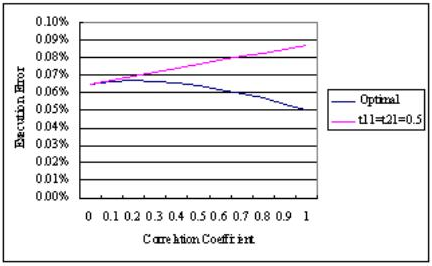
\includegraphics[width=10cm,height=6cm]{fg_s6n.png}
\end{center}
\caption[Execution error for two stocks]{{\bf Execution error for two stocks.}
 \quad This graph shows the standard deviation of VWAP execution errors ($y$-axis) for different price correlations
($x$-axis).
 Evidently the VWAP execution error becomes smaller when execution times are spread, considering the portfolio
effect.
 It is interesting to note that although the total risk of a portfolio with a positive correlation is larger
than that without correlation, this is not the case for VWAP execution risk.}\label{fg_s6}
\end{figure}


%%%%%%%%%%%%%%%%%%%%
\section{Closing Remarks}\label{sec_s5}
This chapter derives the static optimal execution strategy of a VWAP trade that minimizes the expected squared execution error.  This method is powerful because the optimal execution strategy is determined by an iteration of a single variable optimization, rather than by a multivariable optimization.  Analytical solutions are derived in some cases.  The following results are obtained through our analysis.  For a single-stock trade, if price volatility is independent of market trading volume, the optimal execution strategy is determined only by the expected market trading volume distribution and is independent of expectations regarding the magnitude and time dependency of price volatility.  If price volatility is positively correlated with market trading volume, optimal execution times turn out to lag behind the expected market trading volume distribution.  This is because once price volatility and market trading volume surge, traders have to make considerable trades to track market trading volume while execution times do not matter when these parameters remain small throughout the day.  In a basket trade, execution error can be reduced by spreading out execution times according to the correlation of price movement.  Further, we examine these theoretical results with actual trading data and simulations.

This chapter focuses on static optimization since observed variables such as price volatility and the market trading volume of small orders with low liquidity may contain statistical errors too large to be used in forecasting, and there are some concerns that dynamic optimization is inaccurate.  However, we might be able to predict the behavior of stocks with frequent trades to some extent, and dynamic optimization may reduce execution error further in such cases.  Dynamic optimization is analyzed in Chapter \ref{chap_d}.

For simplicity, this chapter minimizes execution error caused by price movement.  In the real world, however, the direct cost of market impact and the indirect cost of information leakage are certainly significant factors in a VWAP trade.  This issue is left for further analysis.


%%%%%%%%%%%%%%%%%%%%%%%%
\section{Appendix}\label{sec_sappendix}

\subsection{Proof of Proposition \ref{prop_s1}}
The expected square error of the whole VWAP transaction is
\begin{eqnarray*}
   \ex{(VWAP-vwap)^2}
    & = & \ex{\left(\frac{\int_0^T P(s)dV(s)+v(T) \times vwap}{V(T)+v(T)}-vwap\right)^2} \\
    & = & \ex{\left(\frac{\int_0^T P(s)dV(s)-V(T) \times vwap}{V(T)+v(T)}\right)^2} \\
    & = & \ex{\left\{\left(\frac{V(T)}{V(T)+v(T)}\right)\left(\frac{\int_0^T P(s)dV(s)}{V(T)}-\frac{\int_0^T P(s)dv(s)}{v(s)}\right)\right\}^2}.
\end{eqnarray*}
Since $P(s)=\int_0^s dP(t)+P(0)$,
\begin{eqnarray*}
  \int_0^T P(s)dV(s)
  & = & \int_0^T \int_0^s dP(t)dV(s) +\int_0^T P(0)dV(s) \\
  & = & \int_0^T \int_t^T dV(s)dP(t) + P(0)V(T).
\end{eqnarray*}

So,
\begin{eqnarray*}
  \frac{\int_0^T P(s)dV(s)}{V(T)}
  & = & \frac{\int_0^T \int_t^T  dV(s)dP(t)+P(0)V(T)}{V(T)} \\
  & = & \frac{\int_0^T \{V(T)-V(t)\}dP(t)}{V(T)}+P(0)\\
  & = & \int_0^T X(t)dP(t)+P(0).
\end{eqnarray*}
Therefore, the equation above becomes
\begin{eqnarray*}
   &   & \ex{\left\{\left(\frac{V(T)}{V(T)+v(T)}\right)\int_0^T (X(t)-x(t))dP(t)\right\}^2} \\
   & = & \ex{\left(\frac{V(T)}{V(T)+v(T)}\right)^2} \ex{\left\{ \int_0^T (X(t)-x(t))dP(t) \right\}^2} \\
   & & \hspace{2cm} +\cov{\left(\frac{V(T)}{V(T)+v(T)}\right)^2}{\left\{ \int_0^T (X(t)-x(t))dP(s) \right\}^2}.
\end{eqnarray*}

%%%%%%%%%%%%%%%%%
\subsection{Proof of Proposition \ref{prop_s2}}
\begin{eqnarray*}\label{eq_s14}
  \lefteqn{\min\int_0^T \{-2\ex{\sigma(t,V)^2X(t)}x(t)+ \ex{\sigma(t,V)^2}x(t)\}dt} \\
    & = & \min \sum_{k=1}^{v(T)} \int_{t_{k-1}}^{t_k} \{-2 \ex{\sigma(t,V)^2X(t)}x(t)+ \ex{\sigma(t,V)^2}x(t)^2\}dt.
\end{eqnarray*}
The first term is calculated as
\begin{eqnarray*}
  \lefteqn{\sum_{k=1}^{v(T)} \int_{t_{k-1}}^{t_k} \{-2\ex{\sigma(t,V)^2X(s)}x(t)\}dt} \\
    & = & \sum_{k=1}^{v(T)} \int_{t_{k-1}}^{t_k} \left\{-2\ex{\sigma(t,V)^2X(s)}\left(1-\frac{k-1}{v(T)} \right) \right\} dt\\
    & = & \sum_{k=1}^{v(T)} (v(T)-k+1)\int_{t_{k-1}}^{t_k} \left\{-\frac{2
\ex{\sigma(t,V)^2X(s)}}{v(T)}\right\}dt\\
    & = & \sum_{k=1}^{v(T)-1} (v(T)-k)\int_{t_{k-1}}^{t_k} \left\{-\frac{2\ex{\sigma(t,V)^2X(s)}}{v(T)}\right\}dt+\int_0^{t_v} \left\{-\frac{2\ex{\sigma(t,V)^2X(s)}}{v(T)}\right\}dt \\
    & = & \sum_{k=1}^{v(T)-i} (v(T)-k+1-i)\int_{t_{k-1}}^{t_k} \left\{-\frac{2\ex{\sigma(t,V)^2X(s)}}{v(T)} \right\}dt+\sum_{k=v(T)+1-i}^{v(T)} \int_0^{t_k} \left\{-\frac{2\ex{\sigma(t,V)^2X(s)}}{v(T)}\right\}dt \\
    & = & \sum_{k=1}^{v(T)} \int_0^{t_k} \left\{-\frac{2\ex{\sigma(t,V)^2X(s)}}{v(T)}\right\}dt.
\end{eqnarray*}
Also, the second term becomes
\begin{eqnarray*}
   \lefteqn{\sum_{k=1}^{v(T)} \int_{t_{k-1}}^{t_k} \{ \ex{\sigma(t,V)^2}x(t)^2\}dt}\\
    & = & \sum_{k=1}^{v(T)} \int_0^{t_k} \ex{\sigma(t,V)^2}x(t_{k-1})^2 dt-\sum_{k=1}^{v(T)} \int_0^{t_{k-1}} \ex{\sigma(t,V)^2}x(t_{k-1})^2 dt\\
    & = & \sum_{k=1}^{v(T)} \int_0^{t_k} \ex{\sigma(t,V)^2}x(t_{k-1})^2 dt-\sum_{k=1}^{v(T)-1} \int_0^{t_k} \ex{\sigma(t,V)^2}x(t_k)^2 dt\\
    & = & \sum_{k=1}^{v(T)} \int_0^{t_k} \{ \ex{\sigma(t,V)^2}x(t_{k-1})^2\}dt\\
    &   & -\left[ \sum_{k=1}^{v(T)} \int_0^{t_k} \ex{\sigma(t,V)^2}x(t_k)^2 dt+\int_0^{t_0} \ex{\sigma(t,V)^2}x(t_0)^2 dt-\int_0^{t_v} \ex{\sigma(t,V)^2}x(t_v)^2 dt \right]\\
    & = & \sum_{k=1}^{v(T)} \int_0^{t_k} \ex{\sigma(t,V)^2} \{ x(t_{k-1})^2-x(t_k)^2 \}dt\\
    & = & \sum_{k=1}^{v(T)} \int_0^{t_k} \ex{\sigma(t,V)^2} \left\{ \left(\frac{v(T)-k+1}{v(T)}\right)^2-\left(\frac{v(T)-k}{v(T)}\right)^2 \right\} dt\\
    & = & \sum_{k=1}^{v(T)} \int_0^{t_k} \ex{\sigma(t,V)^2}\frac{2(v(T)-k)+1}{v(T)^2} dt.
\end{eqnarray*}
Therefore, (\ref{eq_s14}) becomes
\[
  \min \sum_{k=1}^{v(T)} \int_0^{t_k} \left\{ -\frac{2 \ex{\sigma(t,V)^2X(t)}}{v(T)
\ex{\sigma(t,V)^2}}+\frac{2(v(T)-k)+1}{v(T)^2}\right\} \ex{\sigma(t,V)^2} dt.
\]

%%%%%%%%%%%%%%%%%
\subsection{Proof of Proposition \ref{prop_s3}}
Since $X(t)$ and $x(t)$ are uncorrelated, (\ref{eq_s5}) becomes
\[
  \min \sum_{k=1}^v \int_0^{t_k} \left\{-\frac{2\ex{X(t)}}{v(T)}+\frac{2(v(T)-k)+1}{v(T)^2} \right\}\ex{\sigma(t)^2}dt.
\]
If we represent the integrand as $f_k(t)$, we can prove that this function takes a negative value in $[0,t_{k-1}]$ and turns from negative to positive just once in $[t_{k-1},T]$, and therefore, we can choose $\{t_k^*\}$ at such point.  This is because the function is monotone increasing with respect to $t$, and the sign of the integrand can be checked by 

\[
  \begin{array}{ll}
    \displaystyle f_1(0)=-\frac{1}{v(T)^2}<0, \\
    \displaystyle f_1(T)=\frac{2v(T)-1}{v(T)^2}>0
  \end{array}
\]
when $k=1$.  Also, assuming that the relationship holds for $k-1$, it can be proved for $k$ also since
\[
  \begin{array}{ll}
    \displaystyle f_k(t_{k-1}^*)=f_{k-1}(t_{k-1}^*)-\frac{1}{v(T)^2}<f_{k-1}(t_{k-1}^*) \leq 0, \\
    \displaystyle f_k(T)=\frac{2(v(T)-k)+1}{v(T)}>0.
  \end{array}
\]
So, the relationship holds for all $k$. 
Therefore, $\{t_k^*\}$ is determined to satisfy
\[
  -\frac{2\ex{X(t_k^*)}}{v(T)}+\left\{ \frac{v(T)-k+1}{v(T)} \right\}^2- \left\{ \frac{v(T)-k}{v(T)} \right\}^2 \leq 0,
\]
and
\[
  \lim_{t \downarrow t_k^*} -\frac{2\ex{X(t_k)}}{v(T)}+\left\{ \frac{v(T)-k+1}{v(T)} \right\}^2-
\left\{ \frac{v(T)-k}{v(T)} \right\}^2 \geq 0.
\]
Solving this equation, 
\[
  \ex{X(t_k^*)} \geq \frac{2(v(T)-k)+1}{2v(T)} \geq \lim_{t \downarrow t_k^*} \ex{X(t)}.
\]
We then first assume that $E[X(t)]$ is continuous at $t_k^*$.  In this case, 
\[
  \ex{X(t_k^*)}=\frac{2(v(T)-k)+1}{2v(T)}.
\]
Also, from (\ref{eq_s4}),
\[
  x(t_k^*)=1-\frac{k}{v(T)}=\frac{2v(T)\ex{X(t_k^*)}+1}{2v(T)}.
\]
According to Figure \ref{fg_s1}, $x^*(t)$ takes a constant value over the $t$ range of 
\[
  \ex{X(t_k^*)}-\frac{1}{v(T)}< \ex{X(t)} \leq \ex{X(t_k^*)}
\]
which is equivalent to
\[
  \ex{X(t)} \leq \ex{X(t_k^*)} < \ex{X(t)}+\frac{1}{v(T)}.
\]
Therefore, 
\[
  \frac{2v(T)\ex{X(t)}-1}{2v(T)} \leq x^*(t) < \frac{2v(T)\ex{X(t)}+1}{2v(T)}.
\]
Or equivalently,
\[
  x^*(t)=\frac{\lfloor (2v(T)\ex{X(t)}+1)/2 \rfloor}{v(T)}.
\]
Next, if $\ex{X(t)}$ is not continuous at $t_k^*$, the same argument can be applied.  Specifically, 
\[
  x^*(t_k^*)=\frac{\lfloor (2v(T)\ex{X(t_k^*)}+1)/2 \rfloor}{v(T)}
\]
from left continuity, and also,
\[
  \lim_{t \downarrow t_k^*}x^*(t)=\lim_{t \downarrow t_k^*}\frac{\lfloor (2v(T)\ex{X(t)}+1)/2 \rfloor}{v(T)}.
\]
Therefore, we can conclude that for all $t$,
\[
  x^*(t)=\frac{\lfloor (2v(T)\ex{X(t)}+1)/2 \rfloor}{v(T)}.
\]

%%%%%%%%%%%%%%%%%
\subsection{Proof of Proposition \ref{prop_s5}}
\begin{eqnarray*}
  \lefteqn{\min\sum_{i=1}^N \sum_{j=1}^N W_{ij}\int_0^T \ex{\rho_{ij}\sigma_i\sigma_j(X_i-x_i)(X_j-x_j)}dt}\\
    & = & \min \left[ \sum_{i=1}^N \sum_{j=1}^N W_{ij}\int_0^T \{-\ex{\rho_{ij}\sigma_i\sigma_jX_i}x_j-\ex{\rho_{ij}\sigma_i\sigma_jX_j}x_i+\ex{\rho_{ij}\sigma_i\sigma_j}x_ix_j\}dt \right.\\
    &   & \left. +\sum_{i=1}^N \sum_{j=1}^N W_{ij}\int_0^T \ex{\rho_{ij}\sigma_i\sigma_jX_iX_j}dt \right]\\
    & = & \min \left[ \sum_{i=1}^N \sum_{j=1}^N W_{ij} \sum_{k=1}^{v_i(T)}\int_0^{t_{ik}} \left\{-\frac{2\ex{\rho_{ij}\sigma_i\sigma_jX_j}}{v_i\ex{\rho_{ij}\sigma_i\sigma_j}} \right\} \ex{\rho_{ij}\sigma_i\sigma_j}dt+\int_0^T \ex{\rho_{ij}\sigma_i\sigma_j}x_ix_jdt \right.\\
    &   & \left. +\sum_{i=1}^N \sum_{j=1}^N W_{ij}\int_0^T \ex{\rho_{ij}\sigma_i\sigma_jX_iX_j}dt. \right]
\end{eqnarray*}
Because each series of $\{t_{ik}\}$ is double counted in the series of $\{t_k^{ij}\}$,
\begin{eqnarray*}
  \lefteqn{\min \left[ \sum_{i=1}^N \sum_{j=1}^N W_{ij} \left\{ \sum_{k=1}^{v_i(T)}\int_0^{t_{ik}} \left(-\frac{2\ex{\rho_{ij}\sigma_i\sigma_jX_j}}{v_iE[\rho_{ij}\sigma_i\sigma_j]}\right)\ex{\rho_{ij}\sigma_i\sigma_j}dt \right. \right.} \\
    &   & \left. \left. +\sum_{k=1}^{v_i(T)+v_j(T)}\int_0^{t_k^{ij}}\frac{x_i(t_{k-1}^{ij})x_j(t_{k-1}^{ij})-x_i(t_k^{ij})x_j(t_k^{ij})}{2} \ex{\rho_{ij}\sigma_i\sigma_j}dt \right\} \right]\\
    &   & +\sum_{i=1}^N \sum_{j=1}^N W_{ij}\int_0^T \ex{\rho_{ij}\sigma_i\sigma_jX_iX_j}dt \\
    & = & \min \sum_{i=1}^N \sum_{j=1}^N W_{ij} \sum_{k=1}^{v_i(T)+v_j(T)} \int_0^{t_k^{ij}} \left\{ -\frac{\ex{\rho_{ij}\sigma_i\sigma_jX_j}}{v_i \ex{\rho_{ij}\sigma_i\sigma_j}}+\frac{x_i(t_{k-1}^{ij})x_j(t_{k-1}^{ij})-x_i(t_k^{ij})x_j(t_k^{ij})}{2}\right\}\ex{\rho_{ij}\sigma_i\sigma_j}dt \\
    &   & +\sum_{i=1}^N \sum_{j=1}^N W_{ij}\int_0^T \ex{\rho_{ij}\sigma_i\sigma_jX_iX_j} dt.
\end{eqnarray*}

% 02/05 changed from .emf to n.png.  Native check
% 02/07 modified typos, eq No, etc. by Makimoto
% 03/12 modified according to 03/07 mail
% 03/22 and 03/25 and 03/26 modified

%%%%%%%%%%%%%%%
%   D-VWAP   %%
%%%%%%%%%%%%%%%

%\setcounter{section}{0}

\chapter{Dynamic Optimal Slice of a VWAP Trade}\label{chap_d}


\begin{quote}
{\bf Abstract} \quad This chapter analyzes an optimal execution strategy of a 
VWAP trade by dynamic control and derives an approximating solution. Non-
negative constraint plays an important role in a dynamic strategy because the 
market trading volume ratio may decrease after big news arrives.  If sell order 
is not allowed, the optimal execution delays in order to avoid excessive execution.  
Also, if the market trading volume surges, the trader should hold his execution 
rather than follow the market trading volume.  We confirm execution error 
reduction by actual trading data.


\end{quote}


%%%%%%%%%%%%%%%%%
\section{Introduction}\label{sec_d1}
VWAP stands for volume-weighted average price during a certain trading period, 
and a VWAP trade refers a trade that uses VWAP as a benchmark.  This chapter 
analyzes the dynamic optimal execution strategy of a VWAP trade.  It extends the 
work of Chapter \ref{chap_s} of this study, which analyzes VWAP trade 
statically.  

As VWAP has become an industry standard, related issues acquire popularity.  
From an empirical side, numerous studies have been done on the relationship 
between price volatility and market trading volume since Clark's (1973) seminal 
paper, including Epps and Epps (1976), Tauchen and Pitts (1983).  Karpoff (1987) 
summarizes these results, and Andersen (1996) proposes a modified model.  These 
studies, in general, support the existence of a positive correlation between 
price volatility and market trading volume and the autocorrelation of themselves 
because surprising news boosts both price volatility and market trading volume.  
Besides, Jain and Joh (1988), Admati and Pfleiderer (1988), Foster and 
Viswanathan (1990), and Chan et al.~(1995) study intraday data and find
a
``U-shaped effect," i.e., within a single day, price volatility and market trading 
volume tend to be higher at the opening and closing than in the middle of a 
trading session. 

Based on these findings, Chapter \ref{chap_s} of this study analyzes optimal 
execution of a VWAP trade.  In executing market trades, a VWAP trader wishes to 
get the average execution price as close to the market VWAP as possible to avoid 
price movement risk.  To do so, a VWAP trader slices a whole trade into small 
executions and tries to spread the executions in a well-balanced manner over the 
trading period, which makes VWAP trades rather labor intensive.  Therefore, it 
often makes sense to build a standard strategy, and execute trades automatically 
according to it.  Although Chapter \ref{chap_s} of this study obtains several 
important implications caused by the correlation between trading volume and 
price volatility, the strategy is optimized statically due to statistical, 
computational, and analytical difficulty.  

However, we might be able to predict the behavior of stocks with frequent trades 
to some extent.  Further, because economic impact tends to be large for such 
stocks, dynamic optimization may reduce considerable execution error further in 
such cases.  Also, it is computationally feasible to apply dynamic control for 
few selected large orders.  Besides, if sell order is not allowed, it is expected that the dynamic optimal execution delays in order to avoid excessive execution.  Therefore, this chapter employs dynamic programming 
and allows traders to change their strategies in the middle of the day after the 
true market trading volume is observed.  

This chapter is organized as follows.  Section \ref{sec_d2} formulizes the 
optimal strategy, and Section \ref{sec_d3} derives the solution.  Finally, 
Section \ref{sec_d4} concludes the analysis.

\section{Formulization of the Optimal Slicing}\label{sec_d2}
Imagine a discrete time frame $t=0,1,\cdots,T$ and a case in which a trader buys 
a certain number of shares and tries to get the average purchase price as close 
as possible to the market VWAP during the trading period from time 1 to time 
$T$.  Let $P_t$ denote the market price at $t\ (t=0,\cdots,T)$, and define
\[
  \Delta P_t \define P_t-P_{t-1}, \qquad t=1,2,\cdots,T.
\]
Let $\Delta v_t$ denote the trader's execution volume at time $t$, and define
\[
  v_t \define \sum_{s=1}^t \Delta v_s, \qquad t=1,2,\cdots,T; \qquad\qquad 
v_0=0.
\]
Also, let $\Delta V_t$ denote the market trading volume at time $t\ 
(t=1,\cdots,T)$ excluding the trader's, and define
\[
  V_t \define \sum_{s=1}^t \Delta V_s, \qquad t=1,2,\cdots,T; \qquad\qquad 
V_0=0,\ \ a.e.
\]
Define the filtration generated by $\{ P_t;\; t=0,1,\cdots,T \}$ and $\{ V_t;\; 
t=0,1,\cdots,T \}$ as
\[
  \calF_t \define \sigma \{ (P_s, V_s); \; s=0,1,\cdots, t \}, \qquad 
t=0,1,\cdots,T.
\]
Under this framework, VWAP trades are executed with the following constraints.

\begin{description}
 \item[(Constraint 1)] At time 0, the trader knows the exogenous whole trade 
size $v_T$, which has to be completed by time $t=T$.
 \item[(Constraint 2)] The trader can submit only buy orders but not sell 
orders, which we call non-negative constraint henceforth.
\[
 0 = v_0 \leq v_1 \leq v_2 \leq \cdots \leq v_{T-1} \leq v_T.
\]
\item[(Constraint 3)] When the trader determines the controllable variable, the 
execution volume $\Delta v_t$ at time $t$, only information up to time $t-1$ is 
available, i.e., $\{ v_t \}$ should be $\{ \calF_t \}$-predictable.
\end{description}
A trader's VWAP is expressed as
\[ %\begin{equation}\label{eq_d1}
  vwap=\frac{\sum_{t=1}^T P_t \Delta v_t}{v_T}.
\] %\end{equation}
Also, the market VWAP excluding the traders' is
\[ %\begin{equation}\label{eq_d2}
  VWAP=\frac{\sum_{t=1}^T P_t \Delta V_t}{V_T}.
\] %\end{equation}
Therefore, the VWAP of the whole market is
\[ %\begin{equation}\label{eq_d3}
  TVWAP=\frac{\sum_{t=1}^T P_t (\Delta V_t + \Delta v_t)}{V_T+v_T}.
\] %\end{equation}
Assume that the trader's execution volume is sufficiently small compared to 
market tradng volume.  Thus, we make the following approximation.

\begin{approximation}\label{appr_d1}
 \quad $V_T/(V_T+v_T) \approx 1,\ \ a.e.$
\end{approximation}

Under this approximation,  
\begin{eqnarray*}
  TVWAP - vwap
   & = & \frac{1}{V_T+v_T} \sum_{t=1}^T P_t \Delta V_t - 
\frac{V_T}{(V_T+v_T)v_T}
         \sum_{t=1}^T P_t \Delta v_t \\
   & \approx & \frac{1}{V_T} \sum_{t=1}^T P_t \Delta V_t - \frac{1}{v_T}
         \sum_{t=1}^T P_t \Delta v_t.
\end{eqnarray*}
Define $y_t \define v_t/v_T\ (t=0,1,\cdots,T)$, and we consider $\{ y_s \}$ as 
the controllable variable rather than $\{ v_s \}$.  The constraints can be 
rewritten as 
\begin{description}
 \item[(Constraint 1')] $y_T=1$.
 \item[(Constraint 2')] $0=y_0 \leq y_1 \leq y_2 \leq \cdots \leq y_{T-1} \leq 
y_T=1$.
 \item[(Constraint 3')] $\{ y_s \}$ is $\{ \calF_s \}$-predictable.
\end{description}
Note that $\displaystyle \{\frac{V_t}{V_T}\}$ is $\calF_T$-measurable but not 
$\{ \calF_t \}$-adapted.
A simple calculation shows that
\begin{eqnarray*}
  \frac{1}{V_T} \sum_{t=1}^T P_t \Delta V_t - \frac{1}{v_T} \sum_{t=1}^T P_t 
\Delta v_t
   & = & \sum_{t=1}^T \left( P_0 + \sum_{s=1}^t \Delta P_s \right)
         \left( \frac{\Delta V_t}{V_T} - \frac{\Delta v_t}{v_T} \right) \\
   & = & \sum_{t=1}^T \sum_{s=1}^t \Delta P_s
         \left( \frac{\Delta V_t}{V_T} - \frac{\Delta v_t}{v_T} \right) \\
   & = & \sum_{s=1}^T \Delta P_s \sum_{t=s}^T
         \left( \frac{\Delta V_t}{V_T} - \frac{\Delta v_t}{v_T} \right) \\
   & = & \sum_{s=1}^T \Delta P_s ( y_{s-1} - \frac{V_{s-1}}{V_T} ) \\
   & = & \sum_{s=1}^{T-1} \Delta P_{s+1} ( y_s - \frac{V_s}{V_T} ).
\end{eqnarray*}
Therefore, 
\begin{eqnarray}
  \ex{(TVWAP-vwap)^2}
   & \approx & \ex{\left( \sum_{s=1}^{T-1} \Delta P_{s+1} (y_s-\frac{V_s}{V_T}) 
\right)^2} \nonumber \\
   & = & \sum_{s=1}^{T-1} \ex{\Delta P_{s+1}^2 (y_s - \frac{V_s}{V_T})^2} 
\nonumber \\ 
   &   & \quad +2 \sum_{s=2}^{T-1} \sum_{t=1}^{s-1}
         \ex{\Delta P_{s+1} \Delta P_{t+1} (y_s-\frac{V_s}{V_T}) (y_t-
\frac{V_t}{V_T})}. \label{eq1_d1}
\end{eqnarray}
Based on empirical analyses such as Jain and Joh (1988), we make the following 
assumptions.

\begin{assumption}\label{ass_d1}

\quad \\
\vspace*{-7mm}

\begin{enumerate}
\item $\Delta P_s=\sigma_{P_s}\epsilon_{P_s}$ where $\epsilon_{P_s}$ is a 
sequence of independent random variables.
\item $\ex{\epsilon_{P_s}}=0, \ex{\epsilon_{P_s}^2}=1 \ (s=1,\cdots,T)$.
\item $\{ \epsilon_{P_s} \}$ is independent of $\{\displaystyle  \frac{V_s}{V_T} 
\}$ and $\{ \sigma_{P_s} \}$.
\end{enumerate}
\end{assumption}
Regarding the first term of (\ref{eq1_d1}), since $y_s$ is
$\calF_{s-1}$-measurabel and independent of $\epsilon_{P_{s+1}}$,
\[ %\begin{equation}
  \ex{\Delta P_{s+1}^2 (y_s-\frac{V_s}{V_T})^2} = \ex{\sigma_{P_{s+1}}^2 (y_s-
\frac{V_s}{V_T})^2}.
\] %\end{equation}
Regarding the second term of (\ref{eq1_d1}), for $s>t$,
\[ %\begin{equation}
  \ex{\Delta P_{s+1} \Delta P_{t+1} (y_s-\frac{V_s}{V_T}) (y_t-\frac{V_t}{V_T})}
   = \ex{\epsilon_{P_{s+1}}} \ex{\epsilon_{P_{t+1}} \sigma_{P_{s+1}} 
\sigma_{P_{t+1}} (y_s-\frac{V_s}{V_T}) (y_t-\frac{V_t}{V_T})} = 0.
\] %\end{equation}
Therefore, the objective function to minimize is given by
\begin{equation}\label{eq1_d2}
  \ex{(TVWAP-vwap)^2} \approx \sum_{s=1}^{T-1} \ex{\sigma_{P_{s+1}}^2 (y_s-
\frac{V_s}{V_T})^2}.
\end{equation}
Note that without the non-decreasing constraint for $\{ y_s \}$, $\displaystyle 
y_s = \cex{\frac{V_s}{V_T}}{\calF_{s-1}}$ is the optimal execution strategy.  
However, in a dynamic strategy, the non-decreasing constraint plays an important 
role in increasing the risk of the excessive execution risk because $\displaystyle \frac{V_s}{V_T}$ may decrease after big news arrives 
and the market trading volume surges while $\displaystyle \ex{\frac{V_s}{V_T}}$ 
is generally monotone increasing in a static strategy.

We decompose the sequence $\displaystyle \{ \frac{V_s}{V_T} \}$, which is not 
observed accurately, into a observable part and an error part as
\[ %\begin{equation}
  \frac{V_s}{V_T} = Y_s + \epsilon_{V_s}, \qquad Y_s \define 
\cex{\frac{V_s}{V_T}}{\calF_s},
  \qquad s=1,2,\cdots,T-1; \qquad\qquad \epsilon_{V_T} = 0, \ \ a.e,
\] %\end{equation}
where we make some regular asumptions for the error part.

\begin{assumption}\label{ass_d2}
\quad \\
\vspace*{-7mm}
\begin{enumerate}
\item $\{ \epsilon_{V_s} \}$ is a sequence of independent random variables.
\item $\ex{\epsilon_{V_s}} = 0\ (s=1,\cdots,T-1)$.
\item $\{ \epsilon_{V_s} \}$ and $\{ Y_s \}$are independent.
\end{enumerate}
\end{assumption}
Since $\{ y_s \}$ is $\{ \calF_{s} \}$-predictable, $\{ y_s \}$ is
independent of $\{ \epsilon_{V_s} \}$.  Therefore, 
\begin{eqnarray}
  \ex{\sigma_{P_{s+1}}^2 (y_s-\frac{V_s}{V_T})^2}
  & = & \ex{\sigma_{P_{s+1}}^2 \{(y_s-Y_s) - \epsilon_{V_s}\}^2} \nonumber \\
  & = & \ex{\sigma_{P_{s+1}}^2 (y_s-Y_s)^2} - 2 \ex{\sigma_{P_{s+1}}^2 (y_s-
Y_s)}\ex{\epsilon_{V_s}} + \ex{\sigma_{P_{s+1}}^2\epsilon_{V_s}^2} \nonumber \\
  & = & \ex{\sigma_{P_{s+1}}^2 (y_s-Y_s)^2} + 
\ex{\sigma_{P_{s+1}}^2\epsilon_{V_s}^2}. \label{eq1_d3}
\end{eqnarray}
Since the second term of (\ref{eq1_d3}), $\ex{\sigma_{P_{s+1}}^2 
\epsilon_{V_s}^2}$, is not controllable, the objective function to minimize in 
(\ref{eq1_d2}) is given by
\[ %\begin{equation}
  \sum_{s=1}^{T-1}  \ex{\sigma_{P_{s+1}}^2 (y_s - Y_s)^2}.
\] %\end{equation}




%%%%%%%%%%%%%%%%%%
\section{Derivation of the Optimal Strategy}\label{sec_d3}

\subsection{Uncorrelated Case}
In order to formulize our optimization problem as a linear Markov decision 
process, we make the following assumption.

\begin{assumption}\label{ass_d3}
 \quad $\{ Y_s \}$ is a Markov chain.
\end{assumption}

The state is represented as the pair of the trader's execution ratio and the 
observed market trading volume ratio $(y_s,Y_s)$.  If we write the state at time 
$s$ as $(y_s,Y_s)=(u,w)$, the execution proceeds as follows:

\begin{enumerate}
 \item According to the value of $Y_s$, $y_{s+1}$ is determined, satisfying $y_s 
\leq y_{s+1} \leq 1$.
 \item Under $Y_s=w$, $Y_{s+1}$ is given by the Markov chain.  Also, $P_{s+1}$ 
is given.
 \item $y_{s+1}$ and $Y_{s+1}$ are executed at price $P_{s+1}$, and the state 
moves to $(y_{s+1}, Y_{s+1})$.
\end{enumerate}
If we define
\[ %\begin{equation}
  C_t^*(u,w) \define \min_{u \leq y_t \leq \cdots \leq y_{T-1} \leq 1} \ \ 
    \sum_{s=t}^{T-1} \cex{\sigma_{P_{s+1}}^2 (y_s - Y_s)^2}{Y_{t-1}=w}, \qquad
    t=1,\cdots,T-1
\] %\end{equation}
where the superscript $*$ denotes the optimal solution henceforth.  Bellman 
equation is given by 
\begin{eqnarray}
  \lefteqn{C_t^*(u,w) = \min_{u \leq y_t \leq 1} \ \ \left\{
     \cex{\sigma_{P_{t+1}}^2 (y_t-Y_t)^2}{Y_{t-1}=w} + 
\cex{C_{t+1}^*(y_t,Y_t)}{Y_{t-1}=w} \right\},} \label{eq_d11} \\
  & & \hspace*{10cm} t=1,2,\cdots,T-2. \nonumber
\end{eqnarray}
Since this formula is still too complicated to generate implications, further 
assumptions are made which are considered reasonable based on standard theories 
and empirical analyses.  Firstly, since $Y_0=0$, $Y_T=1$, and $Y_t$ moves 
randomly between time 0 to $T$, we assume $\{ Y_t \}$ is a Brownian bridge.  Secondly, when we fix $w$, $C_{T-1}^*(u,w)$ is a quadratic function of $u$ over the minimum, or a constant otherwise,  it is natural to approximate $C_t$ quadratically.  
Therefore, we made the following assumptions.
\begin{assumption}\label{ass_d4}
\quad \\
\vspace*{-7mm}
\begin{enumerate}
\item The process of $Y_t$ is represented as
\[ %\begin{equation}\label{eq_d8}
Y_t= \bar \eta_t(Y_{t-1})+\sigma_{Y_t}\epsilon_{Y_t}; \qquad Y_0=0, \quad Y_t=1
\] %\end{equation}
where $\bar \eta_t(\, \cdot\, )$ is a linear function, and $\{ \epsilon_{Y_t} \}$ is 
a sequence of normal random variables that is uncorrelated with 
$\{\epsilon_{P_t}\}$.
\item The market trading volume can be predicted precisely enough that 
$\sigma_{Y_t}$ is sufficiently small.
\item  The value function in the Bellman equation can be written as 
\[ %\begin{equation}\label{eq_d11}
  C_{t+1}^*(u, w) = \left\{
  \begin{array}{ll}
   g_t(w), \\
   (a_t w + b_t u + c_t)^2 + g_t(w), 
  \end{array}
  \right. \quad
  \begin{array}{ll}
    w \geq -\frac{b_tu+c_t}{a_t},\\
    w < -\frac{b_tu+c_t}{a_t}
  \end{array}
\] %\end{equation}
for some coefficients $\{ a_t \}$, $\{ b_t \}$, $\{ c_t \}$, and a function $\{ g_t(w) \}$, which is independent of $u$.
\end{enumerate}
\end{assumption}
Further, let $\{\sigma_{P_t}\}$ be uncorrelated with $\{\epsilon_{Y_t}\}$ in 
this subsection while the correlated case is analyzed in Subsection 
\ref{sec_d32}.  
 In this case, (\ref{eq_d11}) is reduced to
\begin{eqnarray*} %\label{eq_d12}
  C_t^* (u, w)
  & = & \min_{u \leq y_t \leq 1} \left\{
        \ex{\sigma_{P_{t+1}}^2} \cex{(y_t-Y_t)^2}{Y_{t-1}=w}
        + \int_{-\infty}^\infty g_t (\eta) f_t(\eta - \bar \eta_t(w)) d \eta
        \right. \\
  &   & \hspace*{5.5cm} \left.
        + \int_{-\infty}^{-(b_t y_t + c_t)/a_t} (a_t \eta + b_t y_t + c_t )^2
        f_t(\eta - \bar \eta_t(w)) d \eta
        \right\} \\
  & = & \min_{u \leq y_t \leq 1} \left\{ \ex{\sigma_{P_{t+1}}^2} (y_t-\ex{Y_t})^2 + I_t + const \right\}
\end{eqnarray*}
where $\displaystyle f_t(x) \define \frac{1}{\sqrt{2\pi}\sigma_{Y_t}}\mboxexp(-\frac{x^2}{2\sigma_{Y_t}^2})$,
\[
 I_t \define \int_{-\infty}^{-(b_t y_t + c_t)/a_t} (a_t \eta + b_t y_t + c_t )^2
        f_t(\eta - \bar \eta_t(w)) d \eta
\]
and
\[
 const \define \int_{-\infty}^\infty g_t (\eta) f_t(\eta - \bar \eta_t(w)) d \eta
\]
which is constant in $y_t$.
Define $\zeta \equiv \eta-\bar \eta_t(Y_{t-1})$, $z_t \equiv -(b_ty_t+c_t)/a_t-
\bar\eta_t(Y_{t-1})$ and $\displaystyle F_t(x)= \int_{-\infty}^x f_t(y) dy$.
Then,
\[ %\begin{equation}\label{eq_d13}
  I_t = \int_{-\infty}^{z_t}a_t^2(\zeta-z_t)^2f_t(\zeta)d\zeta = a_t^2 \int_{-
\infty}^{z_t} (\zeta^2-2z_t\zeta+z_t^2)f_t(\zeta)d\zeta.
\] %\end{equation}
Using the following equations,
\begin{eqnarray*}
  \int_{-\infty}^{z_t} \zeta f_t(\zeta)d\zeta & = & -\sigma_{Y_t}^2 
f_t(z_t),\label{eq_d14}\\
  \int_{-\infty}^{z_t} \zeta^2 f_t(\zeta)d\zeta & = & \sigma_{Y_t}^2 F_t(z_t)-
\sigma_{Y_t}^2 z_t f_t(z_t),\label{eq_d15}
\end{eqnarray*}
we obtain
\[
  I_t =  a_t^2 \sigma_{Y_t}^2 \{(1+z_t^2)F_t(z_t)+z_t f_t(z_t)\}.
\]
Since $\sigma_{Y_t}$ is small, the risk of the excessive execution is expected to be low, which makes $z_t$ small.  Consequently, $I_t$ can be approximated as
\begin{eqnarray*}
  I_t & \simeq & I_t(0)+I_t'(0)z_t+\frac{I_t''(0)}{2}z_t^2 \\
      & \simeq & \frac{a_t^2 \sigma_{Y_t}^2}{2}+\sqrt{\frac{2}{\pi}}a_t^2 
\sigma_{Y_t}z_t+\frac{a_t^2 \sigma_{Y_t}^2}{2}z_t^2.
\end{eqnarray*}
Therefore, the quadratic approximation of $C_t^*(u,w)$ is given by 
\begin{eqnarray*} %\begin{equation}\label{eq_d21}
 C_t^*(u,w)
  & = & \min_{u \leq y_t \leq 1} \left[
        \left\{ \frac{b_t^2 \sigma_{Y_t}^2}{2}+\ex{\sigma_{P_{t+1}}^2} \right\} y_t^2 \right. \\
  &   & \hspace*{1.5cm}
        \left. +\left\{\left(a_tb_t\sigma_{Y_t}^2-2\ex{\sigma_{P_{t+1}}^2}\right)\bar \eta(w) 
        +b_tc_t\sigma_{Y_t}^2-\sqrt{\frac{2}{\pi}}a_tb_t\sigma_{Y_t}\right\}y_t+const \right] \\
  & = & \left\{
  \begin{array}{ll}
   g_{t-1}(w), \qquad w \geq -\frac{b_{t-1}u+c_{t-1}}{a_{t-1}},\\
   (a_{t-1}w+b_{t-1}u+c_{t-1})^2+g_{t-1}(w),
   \qquad w < -\frac{b_{t-1}u+c_{t-1}}{a_{t-1}}
  \end{array}
  \right.
\end{eqnarray*} %\end{equation}
where the minimum is attained by
\[
  y_t= \max\left\{-\frac{\left(a_tb_t\sigma_{Y_t}^2-2\ex{\sigma_{P_{t+1}}^2}\right)
   \bar \eta(w)+b_tc_t\sigma_{Y_t}^2-\sqrt{\frac{2}{\pi}}a_tb_t\sigma_{Y_t}}{b_t^2 
   \sigma_{Y_t}^2+2\ex{\sigma_{P_{t+1}}^2}}, \ u \right\}.
\] %\end{equation}
Therefore, the optimal $\{ y_t^* \}$ is solved iteratively starting with $y_0^* = 0$.

Specifically, if $\bar \eta(u)=\alpha_t+\beta_t u$, then
\[ %\begin{equation}\label{eq_d24}
  y_t^*= \max(d_tY_{t-1}+e_t, y_{t-1}^*), \qquad t = 1,2,\cdots,T-1
\] %\end{equation}
where 
\begin{eqnarray*}
  y_0^* & = & 0,\\
  d_t & = & -\frac{\left(a_tb_t\sigma_{Y_t}^2-
2\ex{\sigma_{P_{t+1}}^2}\right)}{b_t^2 
\sigma_{Y_t}^2+2\ex{\sigma_{P_{t+1}}^2}}\beta_t,\\
  e_t & = & -\frac{\left(a_tb_t\sigma_{Y_t}^2-
2\ex{\sigma_{P_{t+1}}^2}\right)\alpha_t+b_tc_t\sigma_{Y_t}^2-
\sqrt{\frac{2}{\pi}}a_tb_t\sigma_{Y_t}}{b_t^2 
\sigma_{Y_t}^2+2\ex{\sigma_{P_{t+1}}^2}},\\
  a_T & = & b_T \ \ = \ \ c_T \ \ = \ \ 0,\\
  a_{t-1} & = & \frac{a_tb_t\sigma_{Y_t}^2-2\ex{\sigma_{P_{t+1}}^2}}{2b_{t-
1}}\beta_t,\\
  b_{t-1} & = & \sqrt{\frac{b_t^2 \sigma_{Y_t}^2}{2}+\ex{\sigma_{P_{t+1}}^2}},\\
  c_{t-1} & = & \frac{b_tc_t\sigma_{Y_t}^2}{2b_{t-1}}.
\end{eqnarray*}
For example, if $\{ Y_t \}$ is a Brownian bridge, 
\[ %\begin{equation}\label{eq_d25}
dY_t=dB_t+\frac{1-Y_t}{1-t}dt
\] %\end{equation}
and therefore,
\[ %\begin{equation}\label{eq_d26}
\bar \eta(Y_{t-1})-Y_{t-1}=\frac{1-\bar \eta(Y_{t-1})}{1-t} \Delta t
\] %\end{equation}
or, equivalently,
\[ %\begin{equation}\label{eq_d27}
\bar \eta(Y_{t-1})=\frac{1-t}{1-t+\Delta t}Y_{t-1}+\frac{\Delta t}{1-t+\Delta 
t}. 
\] %\end{equation}
Substituting into the general solution, we obtain
\[ %\begin{equation}\label{eq_d28}
 y_t^* = \max(d_tY_{t-1}+e_t,y_{t-1}^*), \qquad t = 1,2,\cdots,T-1
\] %\end{equation}
where 
\begin{eqnarray*}
  y_0^* & = & 0,\\
  d_t & = & -\frac{\left(a_tb_t\sigma_{Y_t}^2-
2\ex{\sigma_{P_{t+1}}^2}\right)}{b_t^2 
\sigma_{Y_t}^2+2\ex{\sigma_{P_{t+1}}^2}}\frac{1-t}{1-t+\Delta t},\\
  e_t & = & -\frac{\left(a_tb_t\sigma_{Y_t}^2-2\ex{\sigma_{P_{t+1}}^2}\right)\frac{\Delta t}{1-t+\Delta 
t}+b_tc_t\sigma_{Y_t}^2-\sqrt{\frac{2}{\pi}}a_tb_t\sigma_{Y_t}}{b_t^2 
\sigma_{Y_t}^2+2\ex{\sigma_{P_{t+1}}^2}}.
\end{eqnarray*}
As we have mentioned, the non-decreasing constraint plays an important role in a 
dynamic strategy because $Y_t$ may decrease after some big news arrives and the 
market trading volume surges while $\ex{Y_t}$ is generally monotone increasing 
in a static strategy.

In order to avoid excessive execution, $y_t^*$ is expected to be smaller than $Y_t$, 
the optimal strategy without non-decreasing constraint.  Also, once news arrives, 
and $Y_t$ happens to decrease, $y_t^*$ stays constant until $Y_t$ gets back 
large enough.  Therefore, if the market trading volume surges, the trader should 
hold his execution rather than follow the market trading volume.

Figure \ref{fg_d1} shows $Y_t$ and $y_t^*$, and Figure \ref{fg_d2} shows $g_t$ 
and $h_t$ for $\sigma_{Y_t}=1$ and all the $\epsilon_{Y_t}$ are zero.  We can 
see that $y_t^*$ is smaller than $Y_t$ due to the risk that $Y_t$ decreases, 
which delays trade execution.  This is more significant for larger 
$\sigma_{Y_t}$.

\begin{figure}[htbp]
\begin{center}
 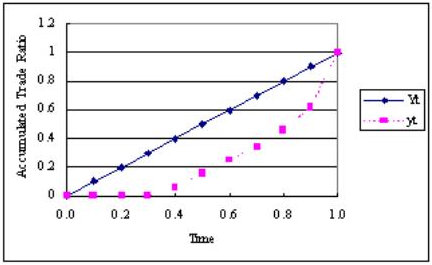
\includegraphics[width=10cm,height=6cm]{fg_d1n.png}
\end{center}
\caption[Numerical example of $Y_t$ and $y_t^*$]{{\bf Numerical example of $Y_t$ 
and $y_t^*$ for $\sigma_{Y_t}=1$ and
where all the $\epsilon_{Y_t}$ are zero.}
 \quad We can see that $y_t^*$ is smaller than $Y_t$ due to the risk that $Y_t$ 
decreases, which delays trade
execution.
 This is more significant for larger $\sigma_{Y_t}$.}\label{fg_d1}
\end{figure}

\begin{figure}[htbp]
\begin{center}
  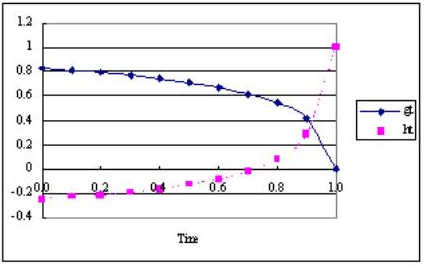
\includegraphics[width=10cm,height=6cm]{fg_d2n.png}
\end{center}
\caption[$g_t$ and $h_t$ for $\sigma_{Y_t}=1$.]{{\bf $g_t$ and $h_t$ for 
$\sigma_{Y_t}=1$.}
 \quad $g_t$ and $h_t$ are deterministic functions that depends only on 
$\sigma_{Y_t}=1$.}\label{fg_d2}
\end{figure}


\subsection{Correlated Case}\label{sec_d32}
If we take correlation between $Y_t$ and $\sigma_{P_t}$ into account, the 
following equation holds.
\begin{eqnarray*}\label{eq_d29}
  \sum_{t=0}^T \ex{(Y_t-y_t)^2 \sigma_{P_{t+1}}^2}
  & = & \sum_{t=0}^T 
\ex{\left\{\frac{\ex{Y_t\sigma_{P_{t+1}}^2}}{\ex{\sigma_{P_{t+1}}^2}}-
y_t\right\}^2 }\ex{\sigma_{P_{t+1}}^2} \nonumber \\
  & = & \sum_{t=0}^T 
\ex{\left\{\ex{Y_t}+\frac{\mbox{Cor}(Y_t,\sigma_{P_{t+1}}^2)\sigma_{Y_t} 
\mbox{Std}(\sigma_{P_{t+1}}^2)}{\ex{\sigma_{P_{t+1}}^2}}-y_t\right\}^2 } 
\ex{\sigma_{P_{t+1}}^2}
\end{eqnarray*}
where $\mbox{Cor}$ and $\mbox{Std}$ stands for the correlation and the standard 
deviation, respectively.  Let the superscript $**$ denote the optimal solution 
of the correlated case.  Then, if $\mbox{Cor}(Y_t,\sigma_{P_{t+1}}^2)$ and 
$\mbox{Std}(\sigma_{P_{t+1}}^2)$ are deterministic, we can solve $y_t^{**}$ just 
as previous argument as
\[ %\begin{equation}\label{eq_d30}
y_t^{**}=y_t^*+\frac{\mbox{Cor}(Y_t,\sigma_{P_{t+1}}^2)\sigma_{Y_t}\mbox{Std}
(\sigma_{P_{t+1}}^2)}{\ex{\sigma_{P_{t+1}}^2}}.
\] %end{equation}

\subsection{Back Tests}
Next, we confirm our theoretical results empirically, using actual intraday data 
from the Tokyo Stock Exchange provided by Nikkei Quick Information Co.~Ltd.  All 
empirical analyses in this chapter are based on trading data from October 2000 
to March 2001 on the 10 stocks with the largest market capitalization.  Data 
from December 29, 2000 and January 4, 2001 are excluded since there was no 
afternoon session on these days.  We chose these large stocks in order to retain 
statistical accuracy since their ticks are frequent and stable.  We believe that 
results can be applied to other stocks since the relationship between price 
volatility and market trading volume is ubiquitous for all stocks as Chan et al. 
(1995) pointed out.  We assume that accumulated market trading volume follows 
the linear difference equation as 
\[ %\begin{equation}\label{eq_d31}
  \bar \eta(u)=\alpha_t+\beta_t u
\] %\end{equation}
and the coefficients $\alpha$ and $\beta$ are obtained through ordinary least 
square regressions where realized $\displaystyle \frac{V_t}{V_T}$ is used as the 
estimate of $Y_t$.  Executions are allocated to periods according to each 
strategy, and the trade is assumed to be executed at the VWAP of the 
corresponding period.  Static strategy is performed in the exactly same manner 
as in Chapter \ref{chap_s}.

Table \ref{table_d1} shows VWAP execution errors for each stock.  We can see 
that dynamic optimization effectively reduces VWAP execution errors.  Also, we 
can further improve our results by taking correlation between accumulated market 
trading volume ratio and price volatility.  In practice, we suffer further price 
changes within the interval and discritization errors due to the minimum trading 
unit, both of which are considered to be proportional to the price volatility as 
in the static optimization in Chapter \ref{chap_s}.

Also, Figure \ref{fg_d3} shows the average delay of the optimal executions, 
$Y_t- y_t^*$ for the uncorrelated case and $Y_t- y_t^{**}$ for the correlated 
case.  We can see that the risk of $Y_t$ decrease and the correlation between 
price volatility and trading volume indeed delays the optimal trade execution.


\begin{table}[htbp]
\begin{center}
\begin{tabular}{|l||c|c|c|} \hline
 & Static & Dynamic & Dynamic (Correlated) \\ \hline\hline
 Takeda & 0.00102 & 0.00071 & 0.00071 \\ \hline
 Matsushita & 0.00095 & 0.00039 & 0.00039 \\ \hline
 Sony & 0.00093 & 0.00044 & 0.00044 \\ \hline
 Toyota & 0.00100 & 0.00059 & 0.00058 \\ \hline
 Honda & 0.00121 & 0.00083 & 0.00083 \\ \hline
 Seven-Eleven Japan & 0.00219 & 0.00167 & 0.00167 \\ \hline
 Mizuho	& 0.00143 & 0.00092 & 0.00092 \\ \hline
 Tokyo-Mitsubishi & 0.00133 & 0.00077 & 0.00076 \\ \hline
 Nomura & 0.00142 & 0.00065 & 0.00064 \\ \hline
 NTT & 0.00176 & 0.00058 & 0.00059 \\ \hline
 NTT Docomo & 0.00128 & 0.00050 & 0.00050 \\ \hline
 Tokyo Electric Power & 0.00065 & 0.00042 & 0.00041 \\ \hline\hline
 Average & 0.00127 & 0.00071 & 0.00070 \\ \hline
\end{tabular}
\end{center}
\caption[Delay of the optimal execution]{{\bf Delay of the optimal execution.}
 \quad This graph shows the delay of the optimal execution from the average 
trading volume ($y$-axis), which coincides with $Y_t- y_t^*$ in the Uncorrelated 
Case and $Y_t- y_t^{**}$ in the Correlated Case in each period ($x$-axis).  We 
can see that the risk of $Y_t$ decrease and the correlation between price 
volatility and trading volume indeed delays the optimal trade 
execution.}\label{table_d1}
\end{table}


\begin{figure}[htbp]
\begin{center}
 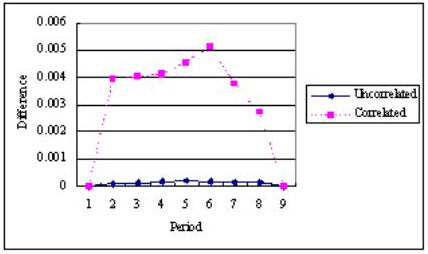
\includegraphics[width=10cm,height=6cm]{fg_d3n.png}
\end{center}
\caption[Graph of VWAP execution errors]{{\bf This graph shows VWAP execution 
errors for each stock.}
 \quad We can see that dynamic optimization effectively reduces VWAP execution 
errors.
 Also, we can further improve our results by taking correlation between 
accumulated market trading volume ratio
 and price volatility.}\label{fg_d3}
\end{figure}


%%%%%%%%%%%%%%%%%%%%
\section{Closing Remarks}\label{sec_d4}
In this chapter we analyzes an optimal execution strategy of a VWAP trade by 
dynamic control and derives approximating solution. Non-negative constraint 
plays an important role in a dynamic strategy because the market trading volume 
ratio may decrease after big news arrives.  If sell order is not allowed, the 
optimal execution delays in order to avoid excessive execution.  Also, if the market 
trading volume surges, the trader should hold his execution rather than follow 
the market trading volume.  We confirm execution error reduction by actual 
trading data.

For simplicity, this analysis studies only one asset execution but not multiple 
asset execution with diversification effect.  Also, estimating the market 
trading volume may not be an easy task even with qualitative judgment.  These 
issues are left for further analysis.

%02/04 changed the title of 7.5.

%%%%%%%%%%%%%%%
%Closing Remarks%%
%%%%%%%%%%%%%%%
\chapter{Closing Remarks}\label{chap_c}
\section{Introduction}\label{sec_c1}
%from (7.1)
As the investment business becomes increasingly competitive, it has turned out that the trade execution also significantly affects investment performance.  As a result, many practitioners start recognizing trade execution as an independent task.  For example, responsibilities of fund managers and traders are clearly separated in the most institutional investors, and principal trades in which security brokers take responsibility of trade execution has become popular for complicated trading needs while execution risk remains investors' responsibility in conventional agency trades.  In contrast, few theoretical researches can be found about trade execution.  Therefore, this study analyzes the optimal trade execution strategies that minimize trading costs for uninformed traders (traders without specific information) whose trading needs are given exogenously. 

In practice, there are mainly two approaches for saving trading costs: 
\begin{enumerate}
\item To balance market impact and volatility risk by referring a fixed price in portfolio or block trades.
\item To mitigate impact of trades by referring volume weighted average price (VWAP henceforth) in VWAP trades.  
\end{enumerate}
These approaches are chosen according to trade size, traders' objectives, circumstances, and so forth.  In our analysis, we divide Approach 1 into long-term execution scheduling problem and short-term order placement problem since it is difficult to analyze Approach 1 as a whole.  Also, in Approach 2, static optimization works well for numerous small orders while dynamic optimization is more suitable for few large orders.  Therefore, the four cases below are analyzed.

\bigskip

\noindent 1. Fixed--Price Trade
\begin{itemize}
\item Execution Schedule
\item Order Placement
\end{itemize}
\noindent 2. VWAP Trade
\begin{itemize}
\item Static Optimization
\item Dynamic Optimization
\end{itemize}

\bigskip

Each issue is explained in the following sections.

%%%%%%%%%%%%%%
\section{Optimal Slice of a Block Trade}\label{sec_c2}
%from(3.6)
Chapter \ref{chap_b} of this study has studied execution scheduling of liquidation of a block trade and formulated it as a static optimization problem.  Based on empirical studies on market microstructure, we have distinguished between temporary market impact and permanent market impact, and assumed that each component to be a linear function of trading volume within moderate volume and time.  Also, we have defined the measure of opportunity cost as standard deviation of price movement, and minimized transaction cost, sum of execution cost and opportunity cost.  Under this framework, we have obtained explicit solutions both for the single-asset case and a multiple-asset portfolio model in the form of pure exponentials.  Further, we have derived an approximation formula when there is a limit to the trading volume executable instantaneously.  

As a result, we have shown that the optimal execution strategy is independent of permanent impact, that optimal execution duration is an increasing function of whole trading size, and that the optimal average cost is an increasing function of whole trading size, price volatility, and temporary impact, and a decreasing function of the limit to instantaneous execution volume, which are all consistent with trading practice and empirical studies.  Specifically, optimal average cost increases as whole trading size to the power of $1/3$ for small orders and $1/2$ for large orders.  Further, it is shown that the transaction cost can be lowered by making order execution late when price movement risk of a portfolio is well diversified.

Our results are immediately applicable to existing risk management framework and provides explicit solution for minimum L-VaR.  Also, although Chapter \ref{chap_b} of this study uses an example of liquidation of a block of common stock, results can be extended over wider problems on liquidation of any large block of assets.

 While Chapter \ref{chap_b} of this study has focused on static optimization, decision change in accordance with new information might be handled by dynamic programming.  Also, this model can reflect more reality by making volatility and market impact time dependent.  Further, it is an interesting issue how to relate order slicing strategy and choice between market order and limit order, and how to control information effect of orders.  These issues are left for further analysis.

%%%%%%%%%%%%%%%%%
\section{Selection of Market and Limit Order}\label{sec_c3}
%from (4.5)
Chapter \ref{chap_l} of this study analyses the optimal selection of market and limit orders in a series of single price batch auctions when the expectation of the limit order book is given.  We derive the analytical solution of a single limit order model for risk neutral traders, and then extend the result for risk averse traders.  Regarding the execution at each period, we find that the optimal limit order size is independent of the whole trade size so as to balance the non--linearity of execution volume and price.  In contrast, the limit order price and the market order size are linear functions in order to balance trading costs across trading periods.  Regarding the execution throughout the trading session, market orders replace limit orders as time passes, and necessity of completing execution grows.  Further, if trading volume and price volatility are larger at the opening and closing of the trading session as in the practical markets, more limit orders are tried at the opening and closing.

Although most traders know the public order book as expectations as in our model, member security brokers are allowed to monitor the public order book without time lags.  So, we evaluate the value of monitoring public order books and provides criteria for selecting stocks to monitor.

Although our results can be extended to multiple limit order models,  mathematical analysis is left for further research.  Besides, while Chapter \ref{chap_l} of this study analyzes batch auctions for simplicity, continuous auction is also of interest.  Also, although Chapter \ref{chap_l} of this study assumes randomness comes only from the number of market orders, the number of limit orders are also stochastic in practice.  Further, we can extend our research to risk averse traders who uses VWAP as a reference price.  Besides, while Chapter \ref{chap_l} of this study performs partial equilibrium type analysis in which public orders are given exogenously, general equilibrium analysis which studies how each trader's strategy interferes is left for further research.

%%%%%%%%%%%%%%%%
\section{Optimal Slice of a VWAP Trade}\label{sec_c4}
%from(5.5)
Chapter \ref{chap_s} of this study derives the static optimal execution strategy of a VWAP trade that minimizes the expected squared execution error.  This method is powerful because the optimal execution strategy is determined by an iteration of a single variable optimization, rather than by a multivariable optimization.  Analytical solutions are derived in some cases.  The following results are obtained through our analysis.  For a single-stock trade, if price volatility is independent of market trading volume, the optimal execution strategy is determined only by the expected market trading volume distribution and is independent of expectations regarding the magnitude and time dependency of price volatility.  If price volatility is positively correlated with market trading volume, optimal execution times turn out to lag behind the expected market trading volume distribution.  This is because once price volatility and market trading volume surge, traders have to make considerable trades to track market trading volume while execution times do not matter when these parameters remain small throughout the day.  In a basket trade, execution error can be reduced by spreading out execution times according to the correlation of price movement.  Further, we examine these theoretical results with actual trading data and simulations.

Chapter \ref{chap_s} of this study focuses on static optimization since observed variables such as price volatility and the market trading volume of small orders with low liquidity may contain statistical errors too large to be used in forecasting, and there are some concerns that dynamic optimization is inaccurate.  However, we might be able to predict the behavior of stocks with frequent trades to some extent, and dynamic optimization may reduce execution error further in such cases.  Dynamic optimization is analyzed in Chapter \ref{chap_d}.

For simplicity, Chapter \ref{chap_s} of this study minimizes execution error caused by price movement.  In the real world, however, the direct cost of market impact and the indirect cost of information leakage are certainly significant factors in a VWAP trade.  This issue is left for further analysis.

%%%%%%%%%%%%%%%%%%%%
\section{Dynamic Optimal Slice of a VWAP Trade}\label{sec_c5}
%from(6.4)
Chapter \ref{chap_d} of this study analyzes an optimal execution strategy of a VWAP trade by dynamic control and derives approximating solution. Non--negative constraint plays an important role in a dynamic strategy because the market trading volume ratio may decrease after big news arrives.  If sell order is not allowed, the optimal execution delays in order to avoid over execution.  Also, if the market trading volume surges, the trader should hold his execution rather than follow the market trading volume.  We confirm execution error reduction by actual trading data.

For simplicity, this analysis studies only one asset execution but not multiple asset execution with diversification effect.  Also, estimating the market trading volume may not be an easy task even with qualitative judgment.  These issues are left for further analysis.

%%%%%%%%%%%%%
\section{Closing Remarks}\label{sec_c6}
%from(7.1)
In practice, all securities trading are carried out through some trade execution, regardless of recognition.  At execution, one of four approaches above are chosen according to assets' characteristics and traders' objectives and circumstances.  In order to make appropriate choice traders have to deeply understand the nature of the alternatives.  

Although few analyses have been made about the optimal trade execution
based on findings of market microstructure, this study derives the
optimal execution strategy in each approach, analyzes its
characteristics, and provides the guidance to the selection of these
approaches.  Therefore, extensive range of application can be expected
for any security trading.


% 03/22 modified
%%%%%%%%%%%%%%%%%%%%%%%%
% References

%\addtolength{\baselineskip}{-1.0\baselineskip}
\begin{thebibliography}{99}
\end{thebibliography}

\begin{description}
 \item[] Abramowitz, M., and I.A. Stegun, ~(1972). ~{\it Handbook of Mathematical Functions}, ~Dover.
 \item[] Admati, A., and P. Pfleiderer, ~(1988). ~A theory of intraday patterns: volume and price variability, ~{\it Review of Financial Studies} 1, Spring, 3--40.
 \item[] Almgren, R., and N. Chriss, ~(1999).~Value under liquidation.~{\it Risk} 12(12),~61--63.
 \item[] Almgren, R., and N. Chriss, ~Optimal execution of portfolio transactions.~{\it Journal of Risk} 3(2), 5--39.
 \item[] Andersen, T.G., ~(1996). Return volatility and trading volume: an information flow interpretation of stochastic volatility, ~{\it Journal of Finance} 71, 169--204.
 \item[] Barclay, M. J., W.G. Christie, J. H. Harris, E. Kandel, and P. H. Schultz,~(1999).~The effects of market reform on the trading costs and depths of Nasdaq stocks.~{\it Journal of Finance} 54, 1--34.
 \item[] BARRA.~(1997).~{\it Market Impact Model Handbook}.
 \item[] Bellman, R.~(1997).~{\it Introduction to Matrix Analysis}, SIAM.
 \item[] Bertsimas, D., and A. Lo, ~(1998). ~Optimal control of execution costs, ~{\it Journal of Financial Markets} 1, 1--50.
 \item[] Biais, B., P. Hillion, and C. Spatt, ~(1995).~An empirical analysis of the limit order book and the order flow in the Paris bourse.~{\it Journal of Finance} 50, 1655--1689.
 \item[] Black, F., and R. Litterman, ~(1991).~Asset allocation: combining investor views  with market equilibrium.~{\it Journal of Fixed Income} 1(2), ~7--18.
 \item[] Chakravarty, S., and C. Holden, ~(1995). An integrated model of market and limit orders, ~{\it Journal of Financial Intermediation} 4, 213--241.
 \item[] Chan, K.C., W.G. Christie, and P.H. Schultz, ~(1995). Market structure and the intraday pattern of bid-Ask Spreads for NASDAQ securities, ~{\it Journal of Business} 68, 35--60.
 \item[] Clark, P.K., ~(1973). A subordinated stochastic process model with finite variance for speculative prices, ~{\it Econometrica} 41, 135--155.
 \item[] Collins, B., and F. Fabozzi, ~(1991).~A methodology for measuring transaction costs.~{\it Financial Analysts Journal} 47, 27--36.
 \item[] Copeland, T.~C., and D. Galai, ~(1983).~Information effects on the bid-ask spread.~{\it Journal of Financial Economics} 7, 229--263.
 \item[] Epps, T.W., and M.L. Epps, ~(1976). The Stochastic dependence of security price changes and transaction volumes: implications for the mixture-of-distributions hypothesis, ~{\it Econometrica} 44, 305--321.
 \item[] Foster, D., and S. Viswanathan, ~(1990). A theory of the interday variations in volume, variance, and trading costs in securities markets, ~{\it Review of Financial Studies} 3, 593--624.
 \item[] Grinold, R., and R. Kahn, ~(1999).~{\it Active Portfolio Management}.~McGraw-Hill Professional Publishing.
 \item[] Hausman, J., A. Lo, and C. MacKinlay, ~(1992). ~An orderd probit analysis of transaction stock prices, ~{\it Journal of Financial Economics} 31, 319--379.
 \item[] Harris, L., and J. Hasbrouck, ~(1996). Market vs. limit orders: the SuperDOT evidence on order submission strategy, ~{\it Journal of Financial and Quantitative Analysis} 31, 213--231.
 \item[] Holthausen, R., R. Leftwich, and D. Mayers, ~(1987).~The effect of large block transactions on security prices: a cross-sectional analysis.~{\it Journal of Financial Economics} 19, 237--268.
 \item[] Hisata, Y., and Y. Yamai, ~(2000).~An analysis on practical liquidity risk measurement.  Institute for Monetary and Economic Studies Discussion Paper 2000-J-3.
 \item[] Jain, P.C., and G. Joh,  ~(1988).~The dependence between hourly
	    prices and trading volume.~{\it Journal of Financial Quantitative Analysis} 23, 269--283.
 \item[] Jorion, P., ~(2000).~{\it Value at Risk}.~McGraw-Hill.
 \item[] Karpoff, J.M., ~(1987). The relation between price changes and trading volume: a survey, ~{\it Journal of Financial and Quantitative Analysis} 22, 109--126.
 \item[] Kawahara, J., ~(1994).  ~Evaluation of execution cost and best execution
 (in Japanese), ~{\it Security Analysts Journal} 12, 32--47.
 \item[] Kawahara, J., and Y. Murase, ~(1993).~Analysis on intraday stock price
 movement.~(in Japanese) {\it Security Analysts Journal} 11, 10--21.
 \item[] Kolmogorov, A.N., and S.V. Fomin, ~(1970).~{\it Introductory Real Analysis}.~Dover.
 \item[] Konishi, H., ~(2002). ~Optimal slice of a VWAP trade, ~{\it Journal of Financial Markets} 5(2) 197--221.
 \item[] Konishi, H., and N. Makimoto, ~(2001). ~Optimal slice of a block trade, ~{\it Journal of Risk} 3(4), 33--51.
 \item[] Konno, H., and A. Wijayanayake,  ~(1998). ~A mean-absolute deviation portfolio optimization model under transaction costs.  Dept. of IE and Management, Tokyo Institute of Technology.
 \item[] Kyle, A. S., ~(1985).~Continuous auctions and insider trading.~{\it  Econometrica} 53, 1315--1335.
 \item[] Lehman, B.N., and D. M. Modest,   ~(1994).~Trading and liquidity on the Tokyo Stock Exchange: a bird's eye view.~{\it  Journal of Finance} 49, 951--984.
 \item[] Mannen, S., and J. Uno, ~(2000).~Basket orders and basis costs.~(in Japanese) {\it NQI Report} 3, 19--22.
 \item[] Markovitz, H., ~(1959). ~{\it Portfolio Selection: Efficient Diversification of Investments}. ~John Wiley \& Sons, Inc.
 \item[] McInish, T. H., and R. A. Wood,  ~(1991).~An analysis of intraday patterns in bid/ask spreads for NYSE stocks. Working Paper, Memphis State University.
 \item[] Parlour, C. A., ~(1998).~Price dynamics in limit order markets.~{\it Review of Financial Studies} 11, 789--816.
 \item[] Perold, A., ~(1988).~The implementation shortfall: paper versus reality.~{\it Journal of Portfolio Management} 14, ~4--9.
 \item[] Protter, P. E., ~(1990). ~{\it Stochastic Integration and Differential Equations: A New Approach}. ~Springer Verlag.
 \item[] Ross, S. A., ~(1976).~The arbitrage theory of capital asset pricing.~{\it Journal of Economic Theory} 13, ~341--360.
 \item[] Sharpe, W., ~(1970). ~{\it Portfolio Theory and Capital Market}. ~McGraw-Hill.
 \item[] Subrahmanyam, A., ~(1991).~Risk aversion, market liquidity, and price efficiency.~{\it Review of Financial Studies} 4(3), 417--442. 
 \item[] Tauchen, G.E., and M. Pitts, ~(1983). The price variability-volume relationship on speculative markets, ~{\it Econometrica} 51, 485--505.
 \item[] Uno, J., and M. Yamada, ~(1993).~Empirical study on market impact.~(in Japanese) {\it Security Analysts Journal} 11, 22--34.
\end{description}


\end{document}
